\documentclass[12pt]{article}
\usepackage{graphicx}
\usepackage {color}
\usepackage{pdfpages}
\usepackage{float}
\usepackage{changebar}
\usepackage{enumitem,amssymb}
\renewcommand{\familydefault}{\sfdefault}
\usepackage[margin=1.2in]{geometry}
\usepackage{graphicx}
\usepackage{wrapfig}
\usepackage[super]{cite}
\usepackage{subcaption}
\usepackage[table]{xcolor}
\usepackage{amsmath}
\usepackage[sort, numbers]{natbib}
\usepackage{multirow}
\usepackage{tabularx}
\usepackage{siunitx}

%%%%%%%%%%%%Defining the margins %%%%%%%%%%%%%%%%%%%%%
\textheight 9.in
\textwidth 6.5in
\topmargin -.5in
\oddsidemargin 0in
\setlength{\parskip}{\smallskipamount}

%%%%%%%%%%%%%%Specific Commands %%%%%%%%%%%%%%%%%%
\newcommand{\eg}{{\em e.g.,}}
\newcommand{\ie}{{\em i.e.,}}
\newcommand{\etc}{{\em etc.,}}
\newcommand{\etal}{{\em et al.}}
\newcommand{\degrees}{{$^{\circ}$}}
\newcommand{\fig}[1]{\textbf{Figure #1}}

%%%%%%%%%%%%%%%%%%%%%%%%%%%% Setting to control figure placement
% These determine the rules used to place floating objects like figures 
% They are only guides, but read the manual to see the effect of each.
\renewcommand{\topfraction}{.9}
\renewcommand{\bottomfraction}{.9}
\renewcommand{\textfraction}{.1}
\renewcommand{\familydefault}{\sfdefault} %setting the san serif font

%%%%%%%%%%%%%%%%%%%%%%%% Line spacing
% Use the following command for ``double'' spacing
%\setlength{\baselineskip}{1.2\baselineskip}
% and this one for an acceptable NIH spacing of 6lpi based on 11pt
%\setlength{\baselineskip}{.9\baselineskip}
% The baselineskip does not appear to work when we include a maketitle
% command in the main file.  Something there must set the line spacing
% If we use this next command, then things seem to work.
\renewcommand{\baselinestretch}{.9}

\setcounter{secnumdepth}{0} %make no numbers but have a table of contents


\begin{document}

\title{Lab 3: ECG Recordings}
\author{Jake Bergquist, u6010393, Partners: Bram Hunt, Genesis Morenorojas }
\maketitle

\section{Introduction}
\par{}
Body surface electrical recordings allows researchers and clinicians to assess the electrical activity of the heart. The use of electrodes to measure and display cardiac electrical activity, known as an electrocardiography (ECG), has been a primary diagnostic and research tool since its invention by Nobel laureate Dr. Willhem Einthoven. During this lab we expored the use of both modern and traditional recording configurations to attain a functional understanding of ECG and vectorcardiography (VCG). By considering measurements between two electrodes, or a lead, we can assess the activity of the heart as a current dipole. We first investigated the use of the three limb leads, first developed by Einthoven. These leads form a roughly equilateral triangle around the heart with three measurement vectors, one set per pair of leads. These leads capture the frontal plane of the heart activity. In an attempt to better understand the 3D extent of the cardiac dipole we used the Frank leads, which form three orthogonal axes of measurement. Utilizing three orthogonal lead measures allows for characterization of the cardiac dipole projected onto each of these axis, and by combining the leads allows for 3D characterization. The third leadset we investigated was the precordial leads. These are six leads across the chest which all use Wilson's Central Terminal as a reference. Wilson's central terminal is made by passing each of the lim lead electrodes through a 5 K\si{\ohm} resistor and then connecting them to reference. By doing so, each of the percordial electrodes can be though of as a unipole recording. These precordial recordings are frequently used clinically as they provide detailed insight into electrical activity of different parts of the heart. Finally we used a full torso body surface potential map dataset to assess how these measurements of the heart may change when the subject changes position. Through our investigations of these lead sets we aim to understand how to interpret these data to understand the electrical activity of the heart, the hearts orientation int he chest, and possibly the viability of the cardiac dipole assumption.
\par{}
ECG and VCG have been used for cardiac diagnostics and research or over a century. By using the geometric relationship between the elecrodes one can construct the heart vector at any point during a heartbeat. Each lead, or electrode pair, measures the projection of th ecardiac vector onto the vector formed by that lead. By combining different leads one can reconstruct the heart vector. By plotting the trajectory of this vector through a heartbeat one gets a VCG vector loop. By analyzing different sections fo the vector loop one can assess the activity during clinically significant parts of the heartbeat such as the QRS complex, the T wave, and the ST segment.
\par{}
\section{Methods}
\par{}
For each lead set the subject sat still, upright, and held their breath for the entire 30 second recording. The subject was allowed to rest in between recordings. 

\subsection{Limb Leads}
\par{}
In lieu of placing the limb leads on the actual limbs we used locations on the torso as these are equivalent and result in higher quality signals. An electrode was attached to the subject's body in the following locations: Left anterior shoulder (LA), right anterior shoulder (RA), left lower ribcage (LL) and right lower rib cage (RL). In each case the electrode was placed over muscle, not bone. The three leads of the Limb leads were constructed from the RA, LA, and LL. V1 positive was LA, and V1 negative was RA. V2 positive was LL and V2 negative was RA. V3 positive was LL, and V3 negative was LA. RL was used as reference for all three leads. 

\par{}



\subsection{Frank Leads}
\par{}
The leads for the Frank Lead set were constructed as follows. For the X component lead the positive terminal was placed on the left midaxillary line below rib 6 and the negative terminal was placed on the right midaxillary line below rib 6. For the Y component the positive terminal was place on the back of the neck to the right of the spine and the negative terminal was connected to the lower left limb electrode. For the Z component the positive terminal was placed on the center of the chest parallel to the 6th rib and the negative lead was connected to the back to the left of the spine at the level of the 6th rib. All electrodes were placed such that they were not directly over bone. The reference for each lead was connected to the lower right lead from the limb lead set.

\subsection{Precordial Leads}
\par{}
The precordial leads were placed as is standard: V1 between rib 4 and 5 on the left on the sternum, V2 between rib 4 and 5 on the right of the sternum, V3 between rib 5 and 6 in the middle of the right pectoral muscle, V4 in between rib 7 and 8 under the nipple, V5 between rib 7 and 8 on the right anterior axillary line, and V6 between rib 7 and 8 on the right mid axillary line. The three limb leads were used to form Wilson's central terminal as a reference by running them through a 5 K\si{\ohm} resistor then connecting them together.

\subsection{Signal Processing}
\par{}
All signals recorded were exported as .csv formatted documents. The CSVs were then imported to matlab and saved in a structure format .mat file. PFEIFER, a preprocessing framework for electrograms, was used to filter, baseline correct, fiducilize, auto fiducilize, and time align the signals recorded.\cite{MacLeod2018_p} Briefly, the raw signals for each intervention were converted by a built in conversion tool, which organizes the potential values recorded into a format PFEIFER requires. Once in a compatible format the signals were imported and  a denoising filter was applied to remove 60 cycle Hz noise.  The first heartbeat from the signal was fiducilized manually by a set of isoelectric points. These isoelectric points were then used to baseline correct the entire recording. Additionally a beat specific baseline correction was applied to the individual beat. The user then fiducilizes the first beat by marking the QRS complex, T wave, and T peak. The manually determined fiducials were then used by PFEIFER to automatically detect any remaining heart beats in the input signal and apply the same beat specific baseline correction and fiducilization. The output are time alligned, fiducilized beats with calculated activation, and recovery times, signal integrals, and beat fiducials.

\par{}
After PFEIFER, the processed beats for each recording site were signal averaged. Because the beats were already time aligned they could easily be collected for each lead recording and averaged over 5 to 20 beats. These signal averaged beats were used for the vector cardiographs. In each case the X components is considered from the left to the right shoulder, the y axis from the top of the chest to the bottom, and the Z from the back to the chest.
In the case of the Frank Lead set the X, Y, and Z components of the vector cardiographs are already defined by the X, Y, and Z lead measurements. In the case of the Precordial recordings to assess the X-Z plane (coronal view) we used V1 as the Z axis and V6 as the X axis. Int he case of the body surface map we chose three orthogonal measurements points to create a lead set like the Frank lead set. The X axis/vector was defined by electrode 53 as the negative terminal and electrode 137 as the positive. The Y axis was defined with electrode 85 as the negative and electrode 96 as the positive. The Z axis was defined with electrode 5 as the negative and electrode 89 as the positive.
\par{}
In the case of the limb leads, assessing the X and Y components of the heart vector was not as straight forward. Because the Limb leads are in a plane there is not the ability to assess the Z component of the heart vector. In order to calculate the X and Y components one must consider how the leads are arranged. Lead I is alligned with the X direction in our coordinate system, thus the X component of the heart vector is composed entirely of lead I. We can calculate the Y component from lead I and lead II as the Y component is projected partially onto lead II but not lead I. Assuming that the triangle formed by leads I, II, and III is equilateral, we can derive the relationship that the Y component of the Heart vector which projects onto lead II is equal to $Hy = (I - 2*II)/\sqrt{3}$. 

\subsection{Vector Cardiographs}
\par{}
For each lead set we constructed vector cardiographs. These show the trajectory of the heart vector through a heart beat. Using the PFEIFER fiducials we were able to separate the pre and post beat isoelectric periods, the QRS complex, the ST segment, and the T wave into separate vectorgraphs. In the case of the Limb leads only the frontal X Y plane can be shown. In the case of the Frank lead set the frontal (X-Y), coronal (X-Z), and sagital (Y-Z) planes were shown. In the case of the precordial leads the coronal plane made by using V1 as the Z component and V6 as the X component. For the body surface maps a 3D plot was presented for each vector graph using all three components of the vector for each recording position.

\section{Results}
\par{}
For each lead set the results are presented as follows. For the Limb lead set a selection of heart beats recorded from each beat is shown after filtering and baseline correction. Note the differences in signal morphology between the leads as well as the odd disturbance in heartrate shown in Figure~\ref{fig:Limb1}. Next several beats for each lead are show in Figure~\ref{fig:Limb2}, followed by the signal averaged beat in Figure~\ref{fig:Limb3}. Note how clean the signals become after averaging. Figure~\ref{fig:Limb4} and Figure~\ref{fig:Limb5} show the VCGs for the lime leads. Figure~\ref{fig:Limb4} illustrates how a VCG is made, but using each computed or measured X and Y component of the heart vector at each time instance and plotting the trajectory of these vectors in the spatial domain. 
\par{}
The same process is repeated for the Frank leads with the exception that, given that the frank leads provides three axes of measurement, a 3D plot (Figures~\ref{fig:Frank3D}\ref{fig:Frank3D_split}) and each orthogonal planar projection (Figure~\ref{fig:Frank_xy} Figure~\ref{fig:Frank_xz} Figure~\ref{fig:Frank_yz}) can be plotted.
\par{}
For the precordial leads after the processing pipeline each beat is already time aligned due to the nature of the fiducilization. These signal averaged and aligned beats are shown in Figure~\ref{fig:PrecordSig}. Using V1 and V6 a coronal plane VCG can be constructed as is shown in Figure~\ref{fig:PrecordVect}.
\par{}
In the case of the body surface potential we chose to use a leadset that mimicked the Frank lead set, with three orthogonal basis vectors. The resulting lead signals were then used to construct the 3D VCGs seen in Figures~\ref{fig:BSP1}, Figure~\ref{fig:BSP2}, Figure~\ref{fig:BSP3}, and Figure~\ref{fig:BSP4}. By exploring these 3D VCGs one can see the planar projections onto all three basis blanes (forntal, coronal, and sagital) as well as explore various other views of the trajectories.

\begin{figure}[H]
	
	\centering
	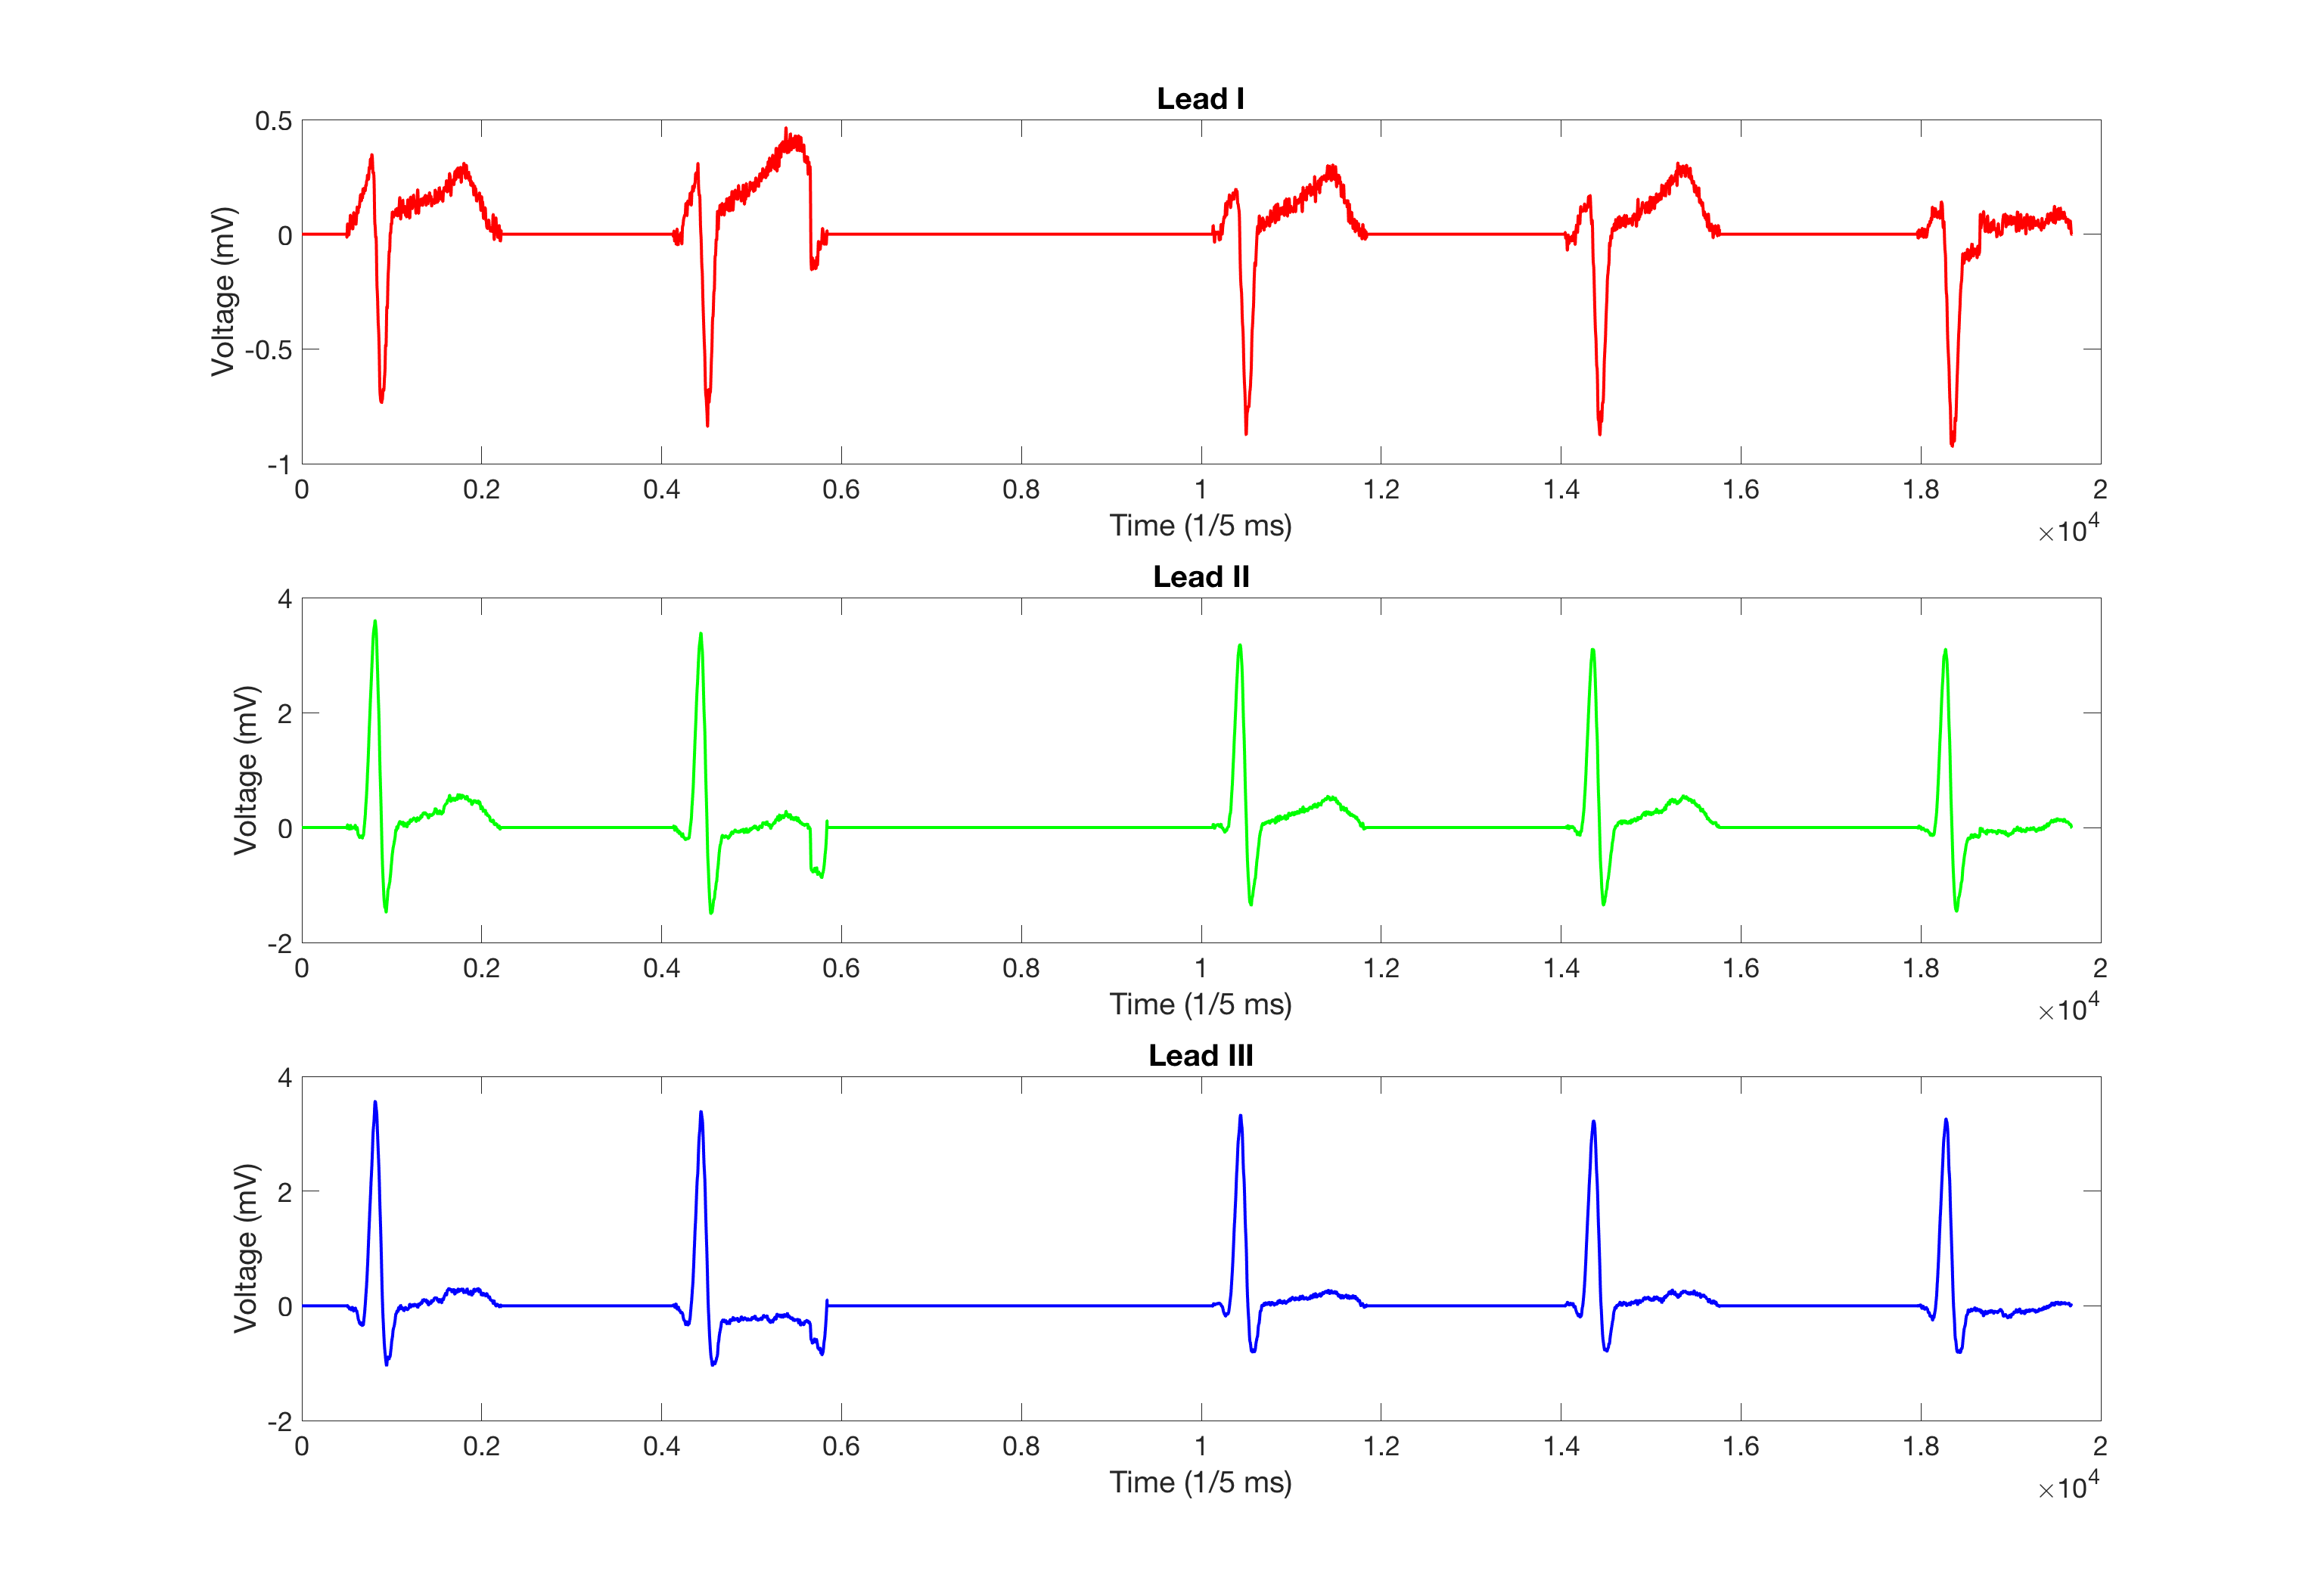
\includegraphics[width = .8\textwidth]{Figures/LimLeads1.png}
	\caption{Baseline Corrected Limb lead recordings.}
	\label{fig:Limb1}
\end{figure}

\begin{figure}[H]
	
	\centering
	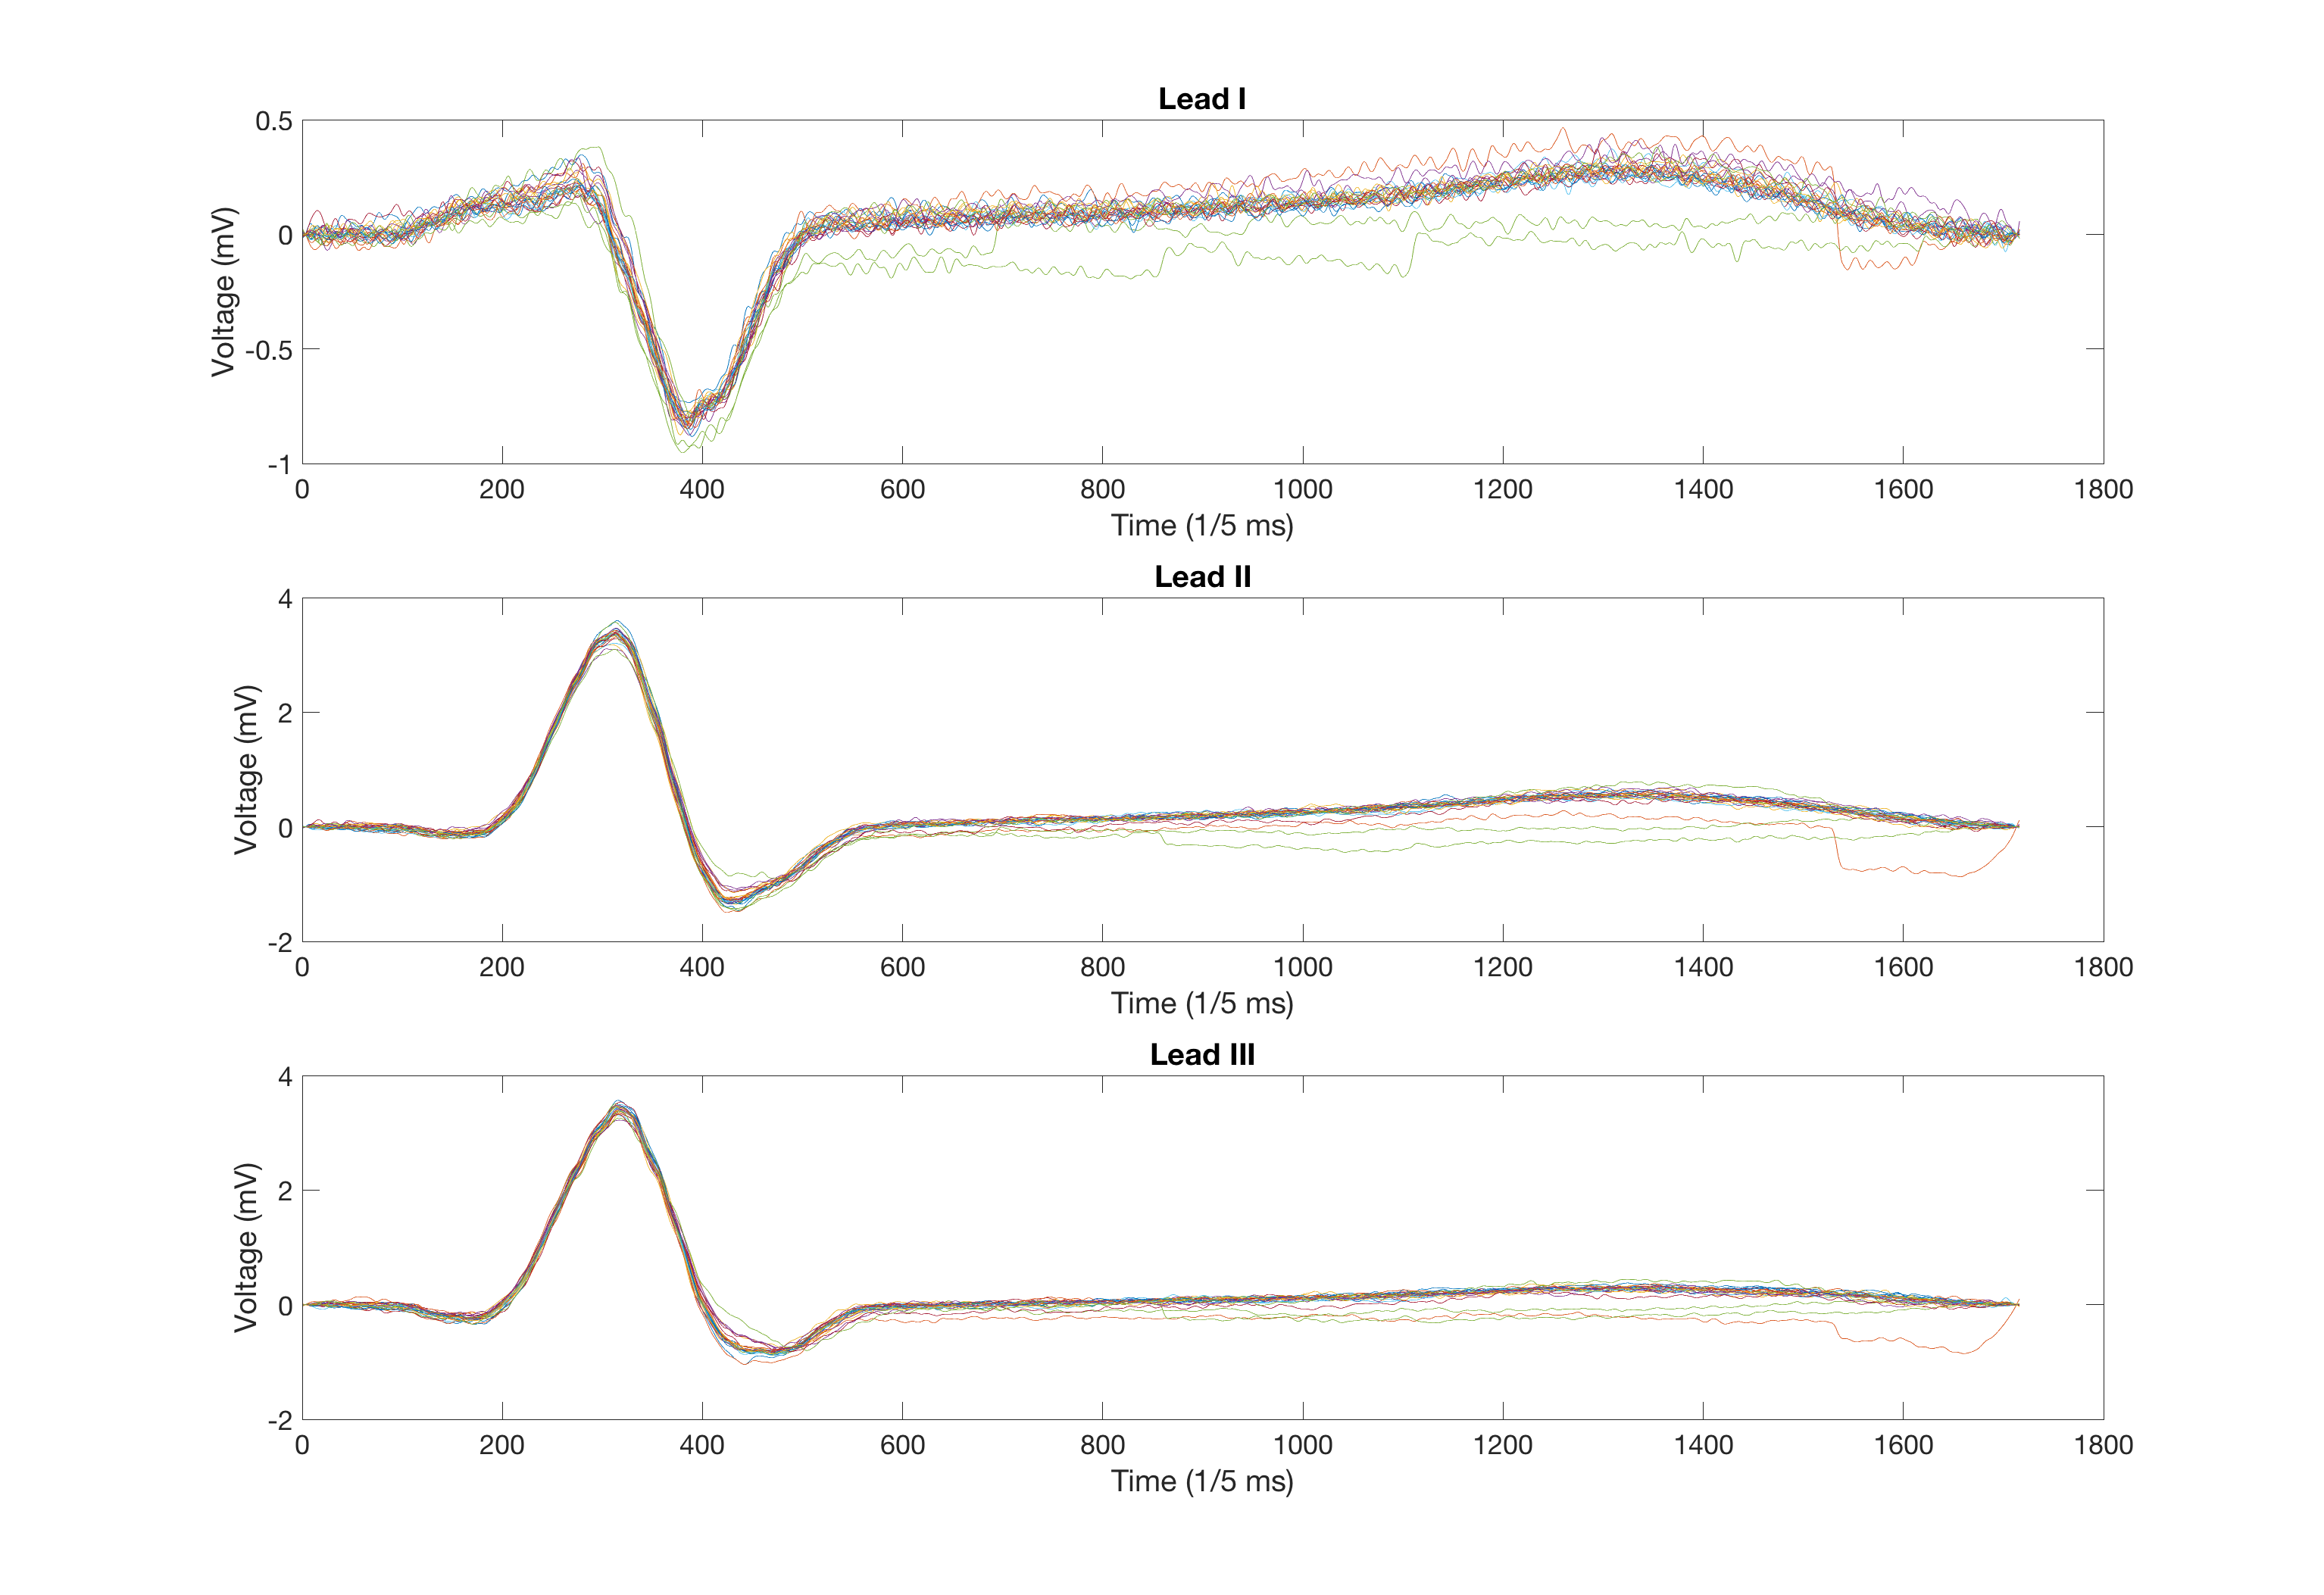
\includegraphics[width = .8\textwidth]{Figures/LimLeads2.png}
	\caption{Limb Lead autofiducilized beats.}
	\label{fig:Limb2}
\end{figure}

\begin{figure}[H]
	
	\centering
	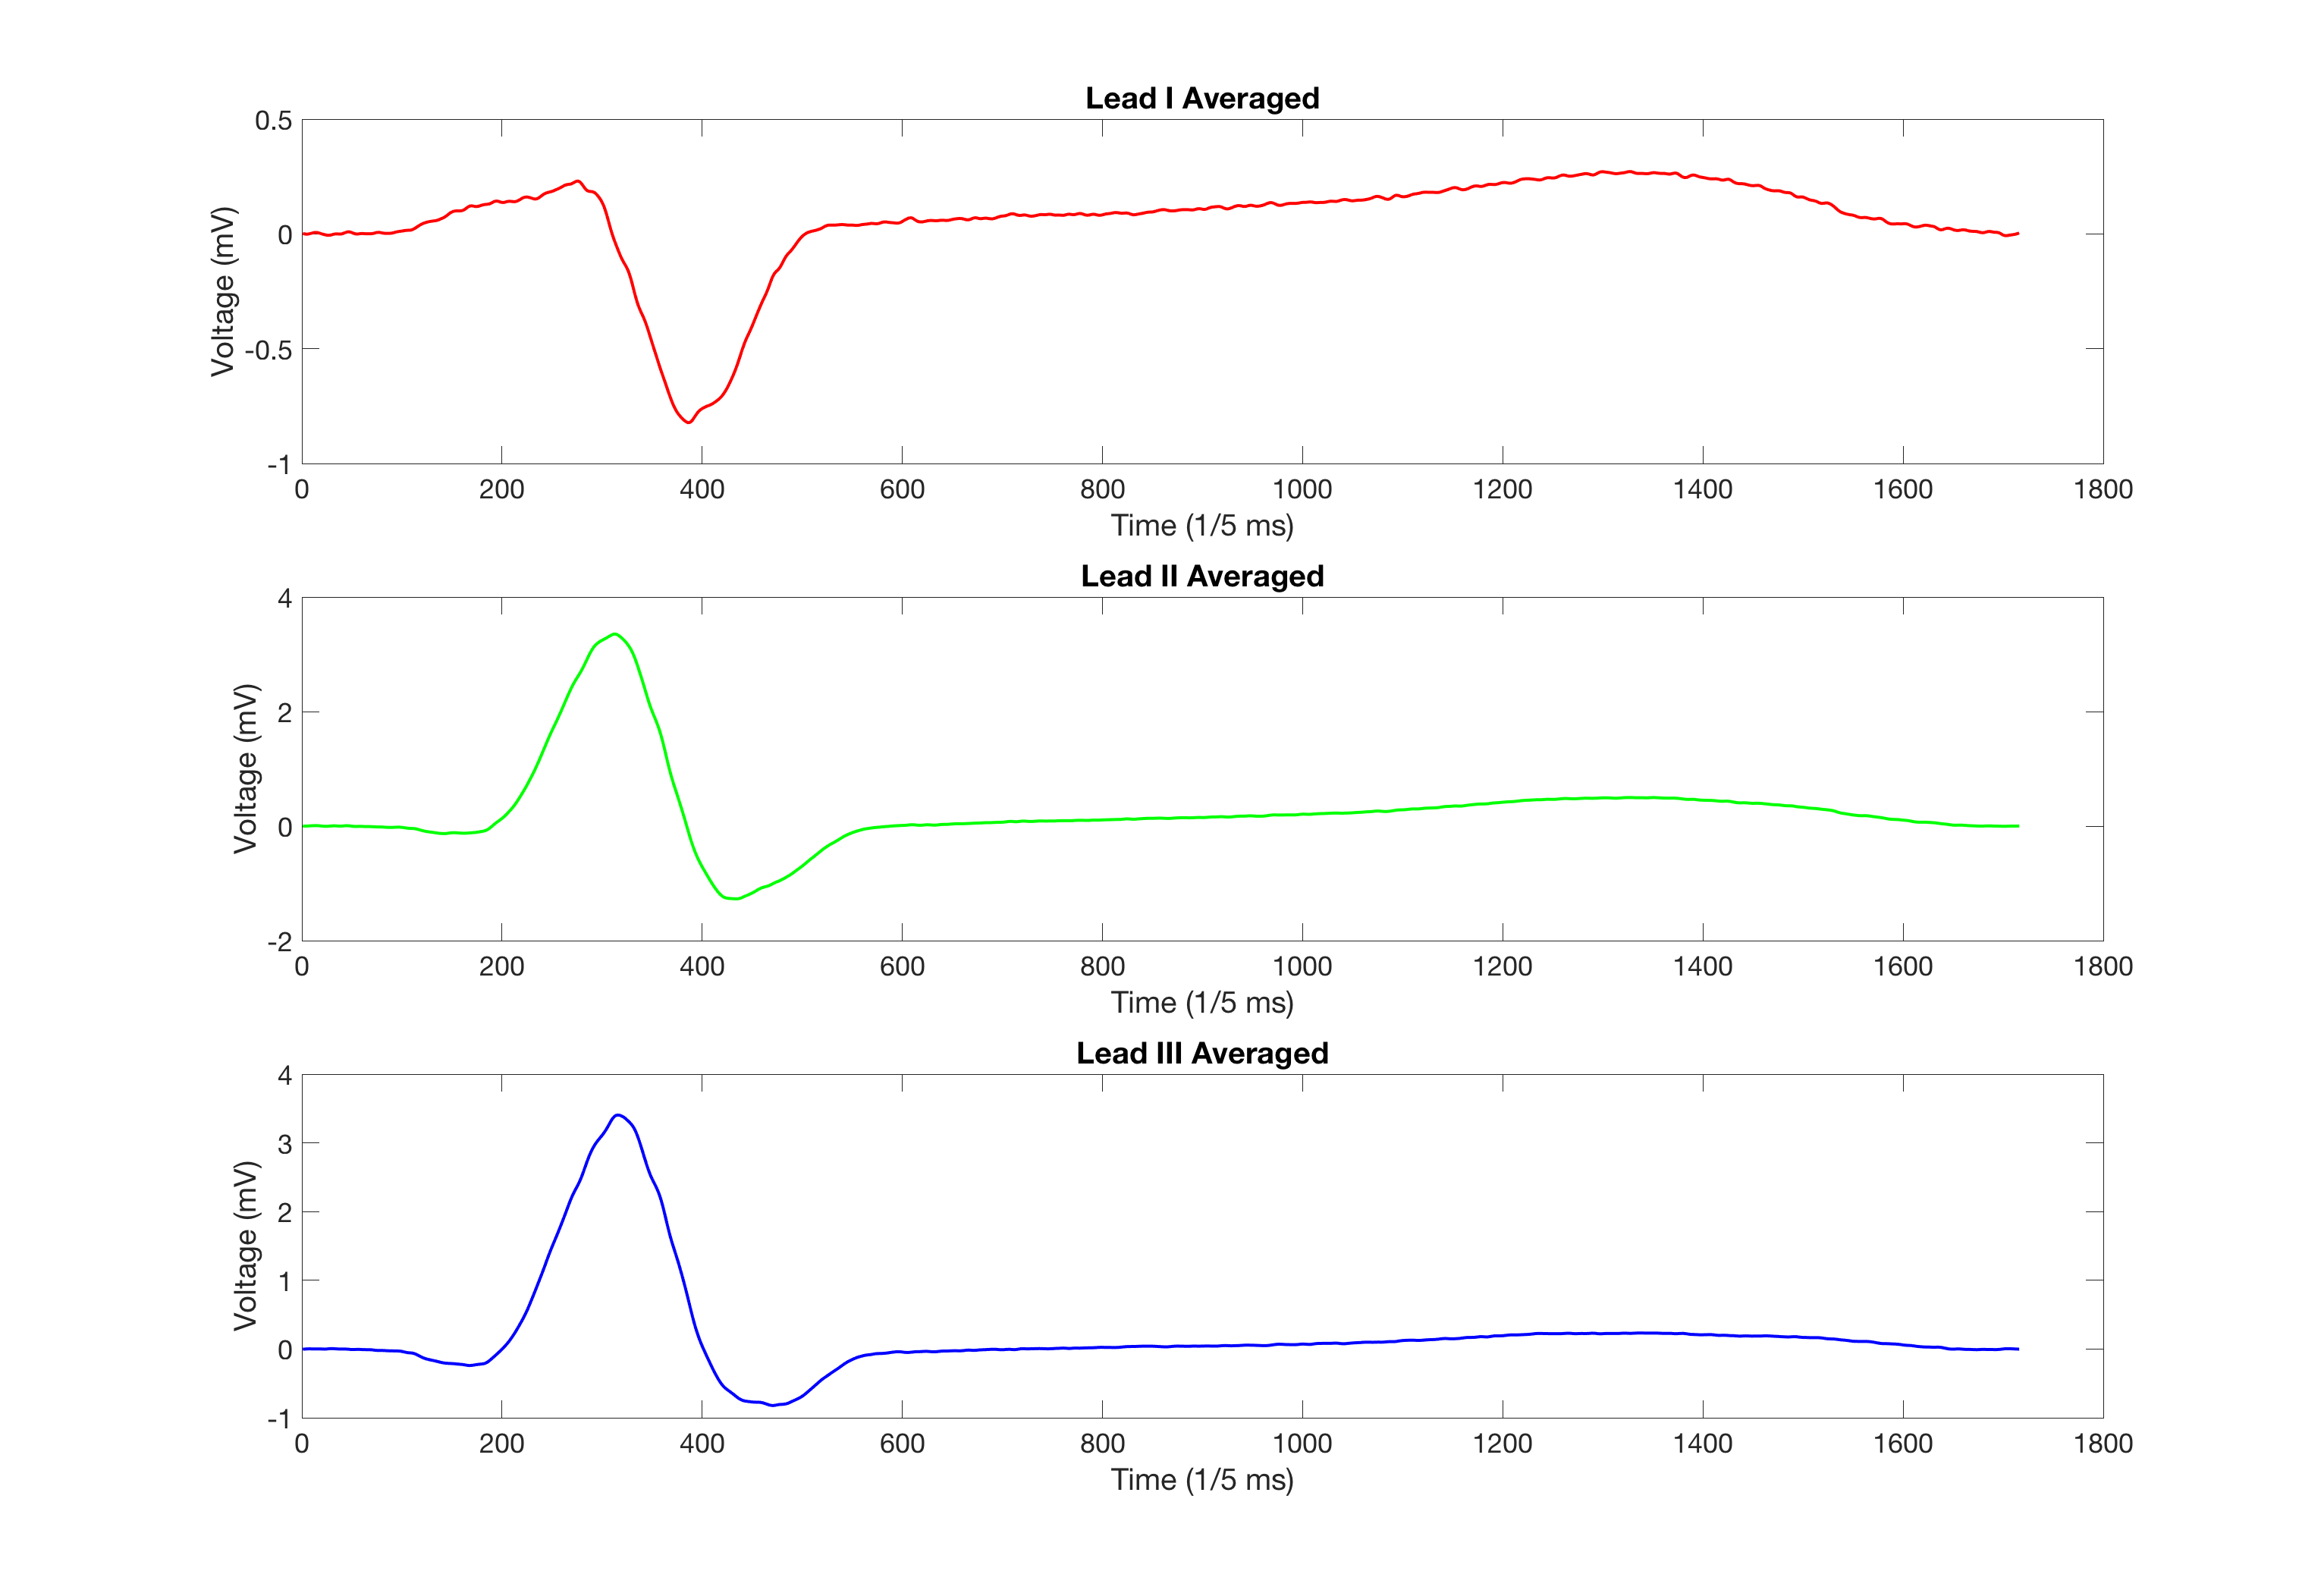
\includegraphics[width = .8\textwidth]{Figures/LimLeads3.png}
	\caption{Limb lead signal averaged beats.}
	\label{fig:Limb3}
\end{figure}

\begin{figure}[H]
	
	\centering
	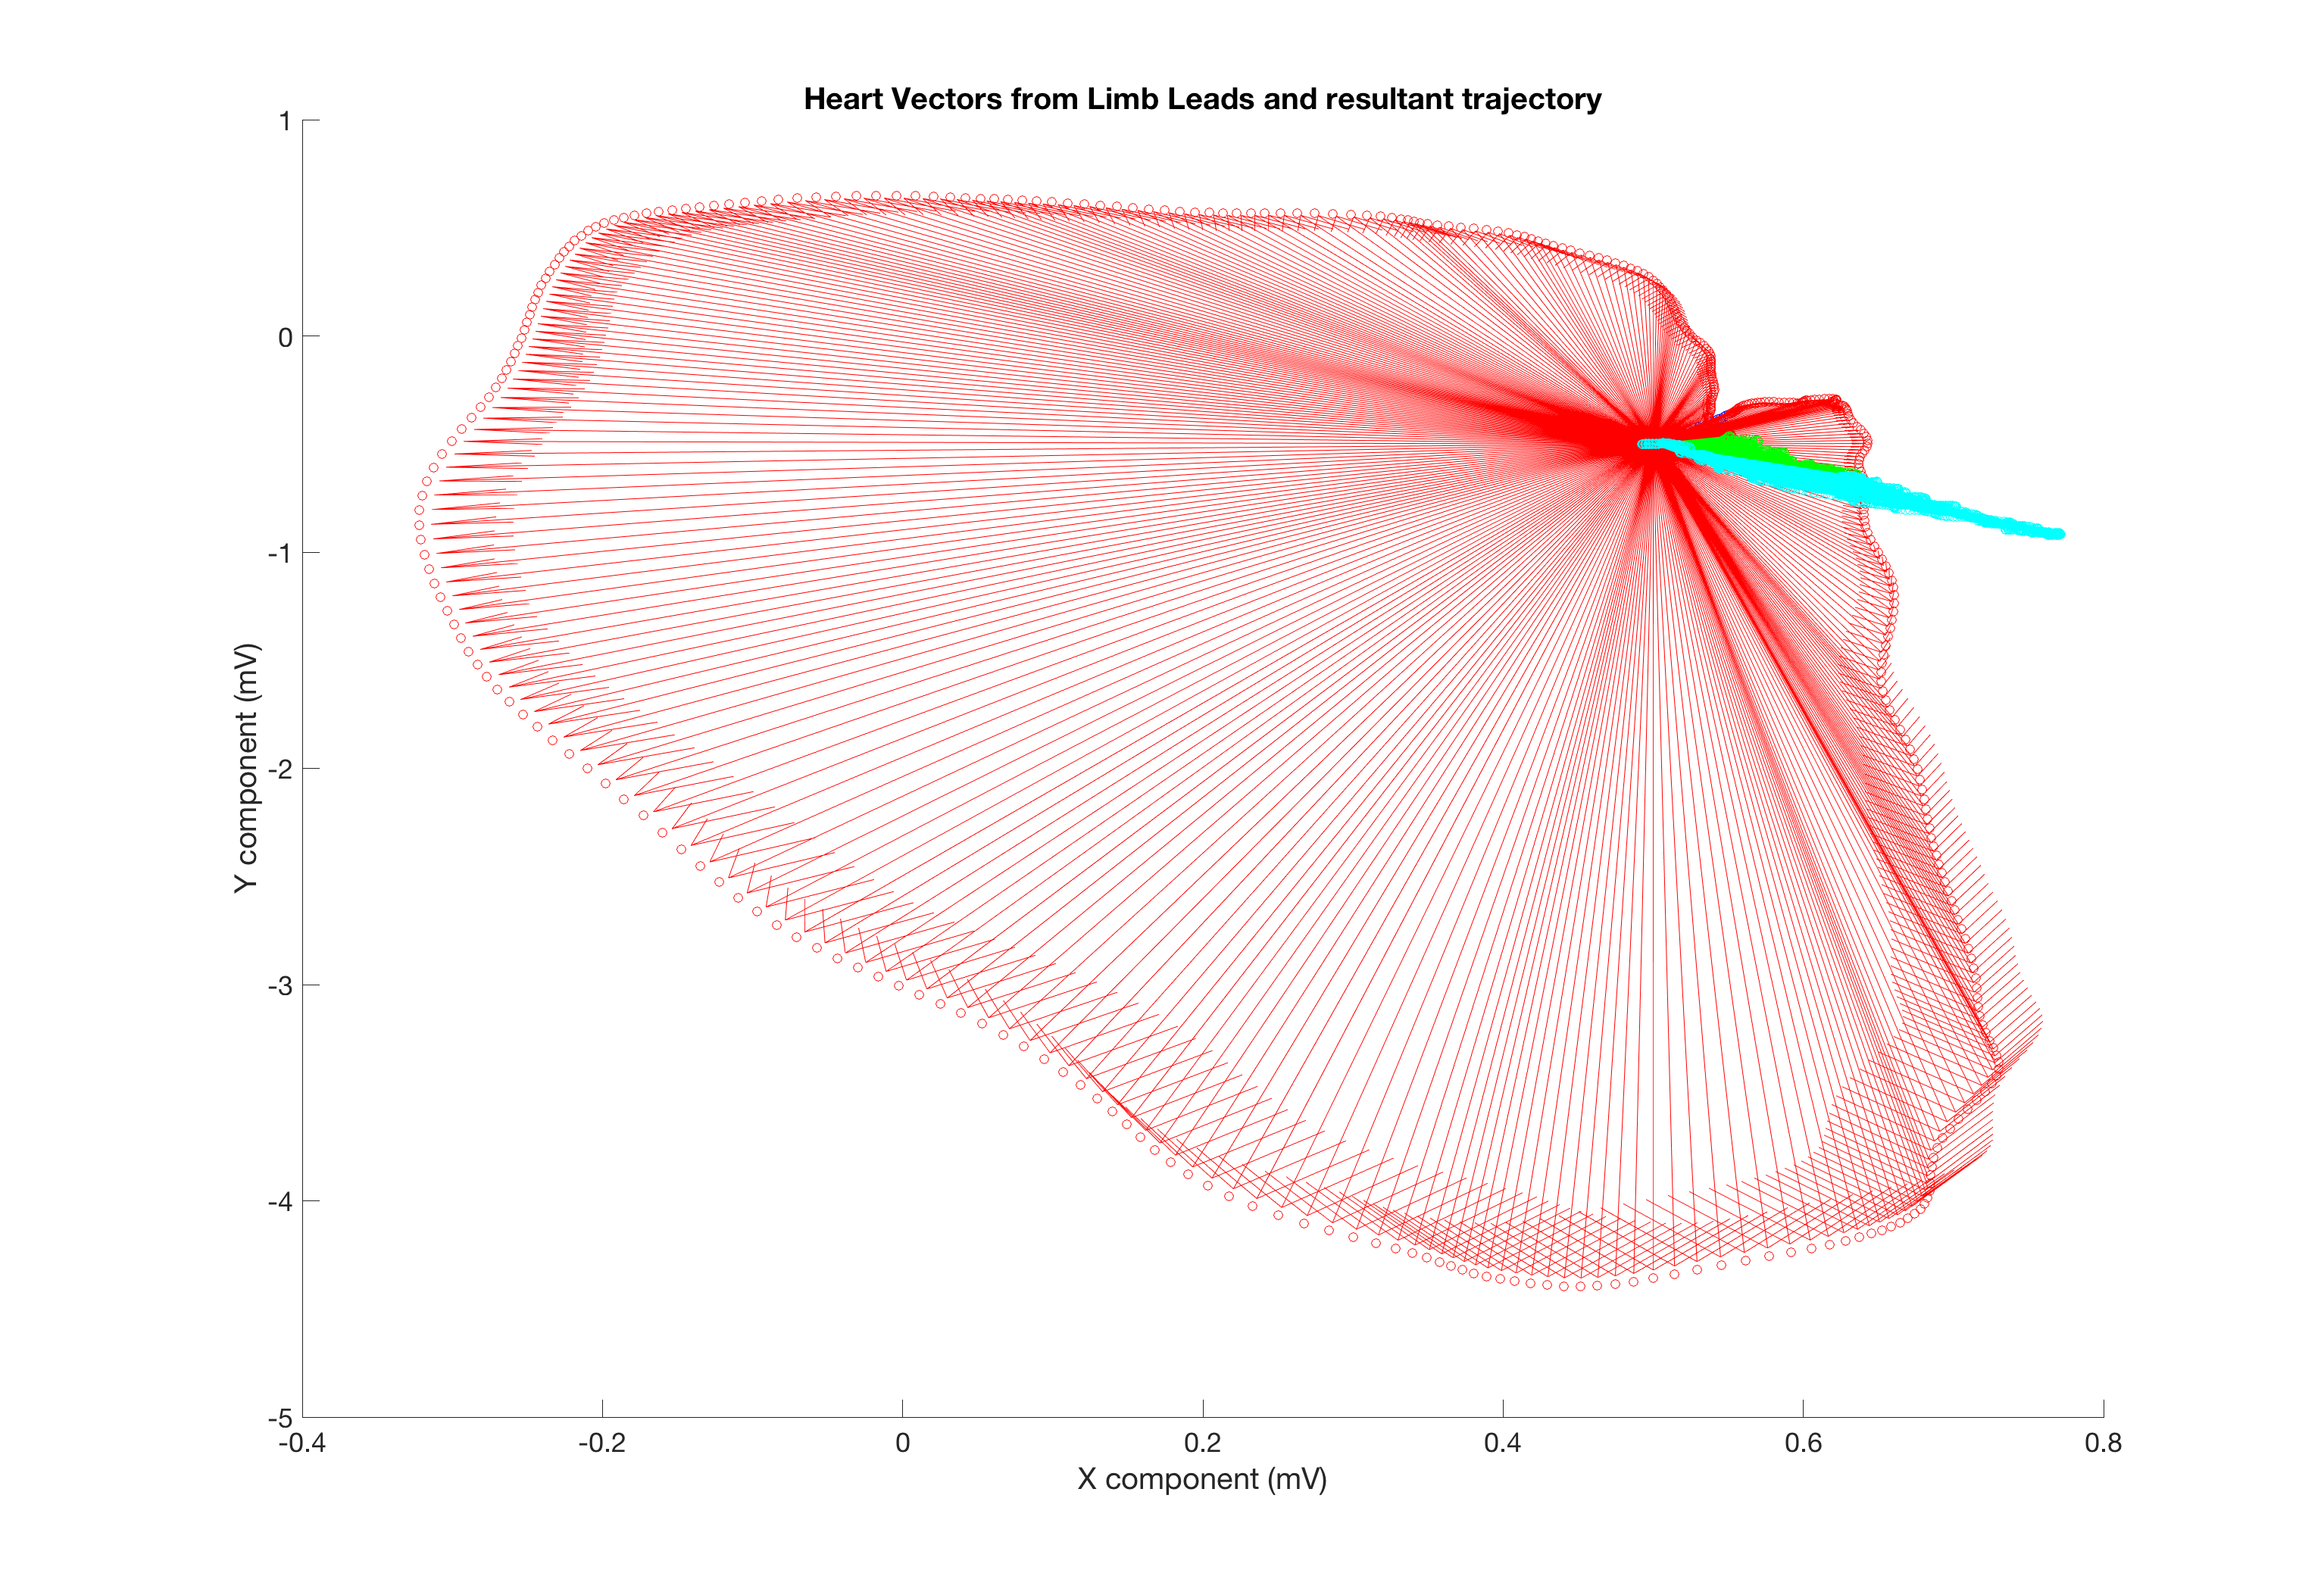
\includegraphics[width = .8\textwidth]{Figures/LimLeads4.png}
	\caption{Full Vectrocardiograph for the limb leads H vector. Plotted in circles are the trajectories and with arrows are thr vectors. QRS in Red, ST segment in green, T wave in cyan, isoelectric in blue. }
	\label{fig:Limb4}
\end{figure}

\begin{figure}[H]
	
	\centering
	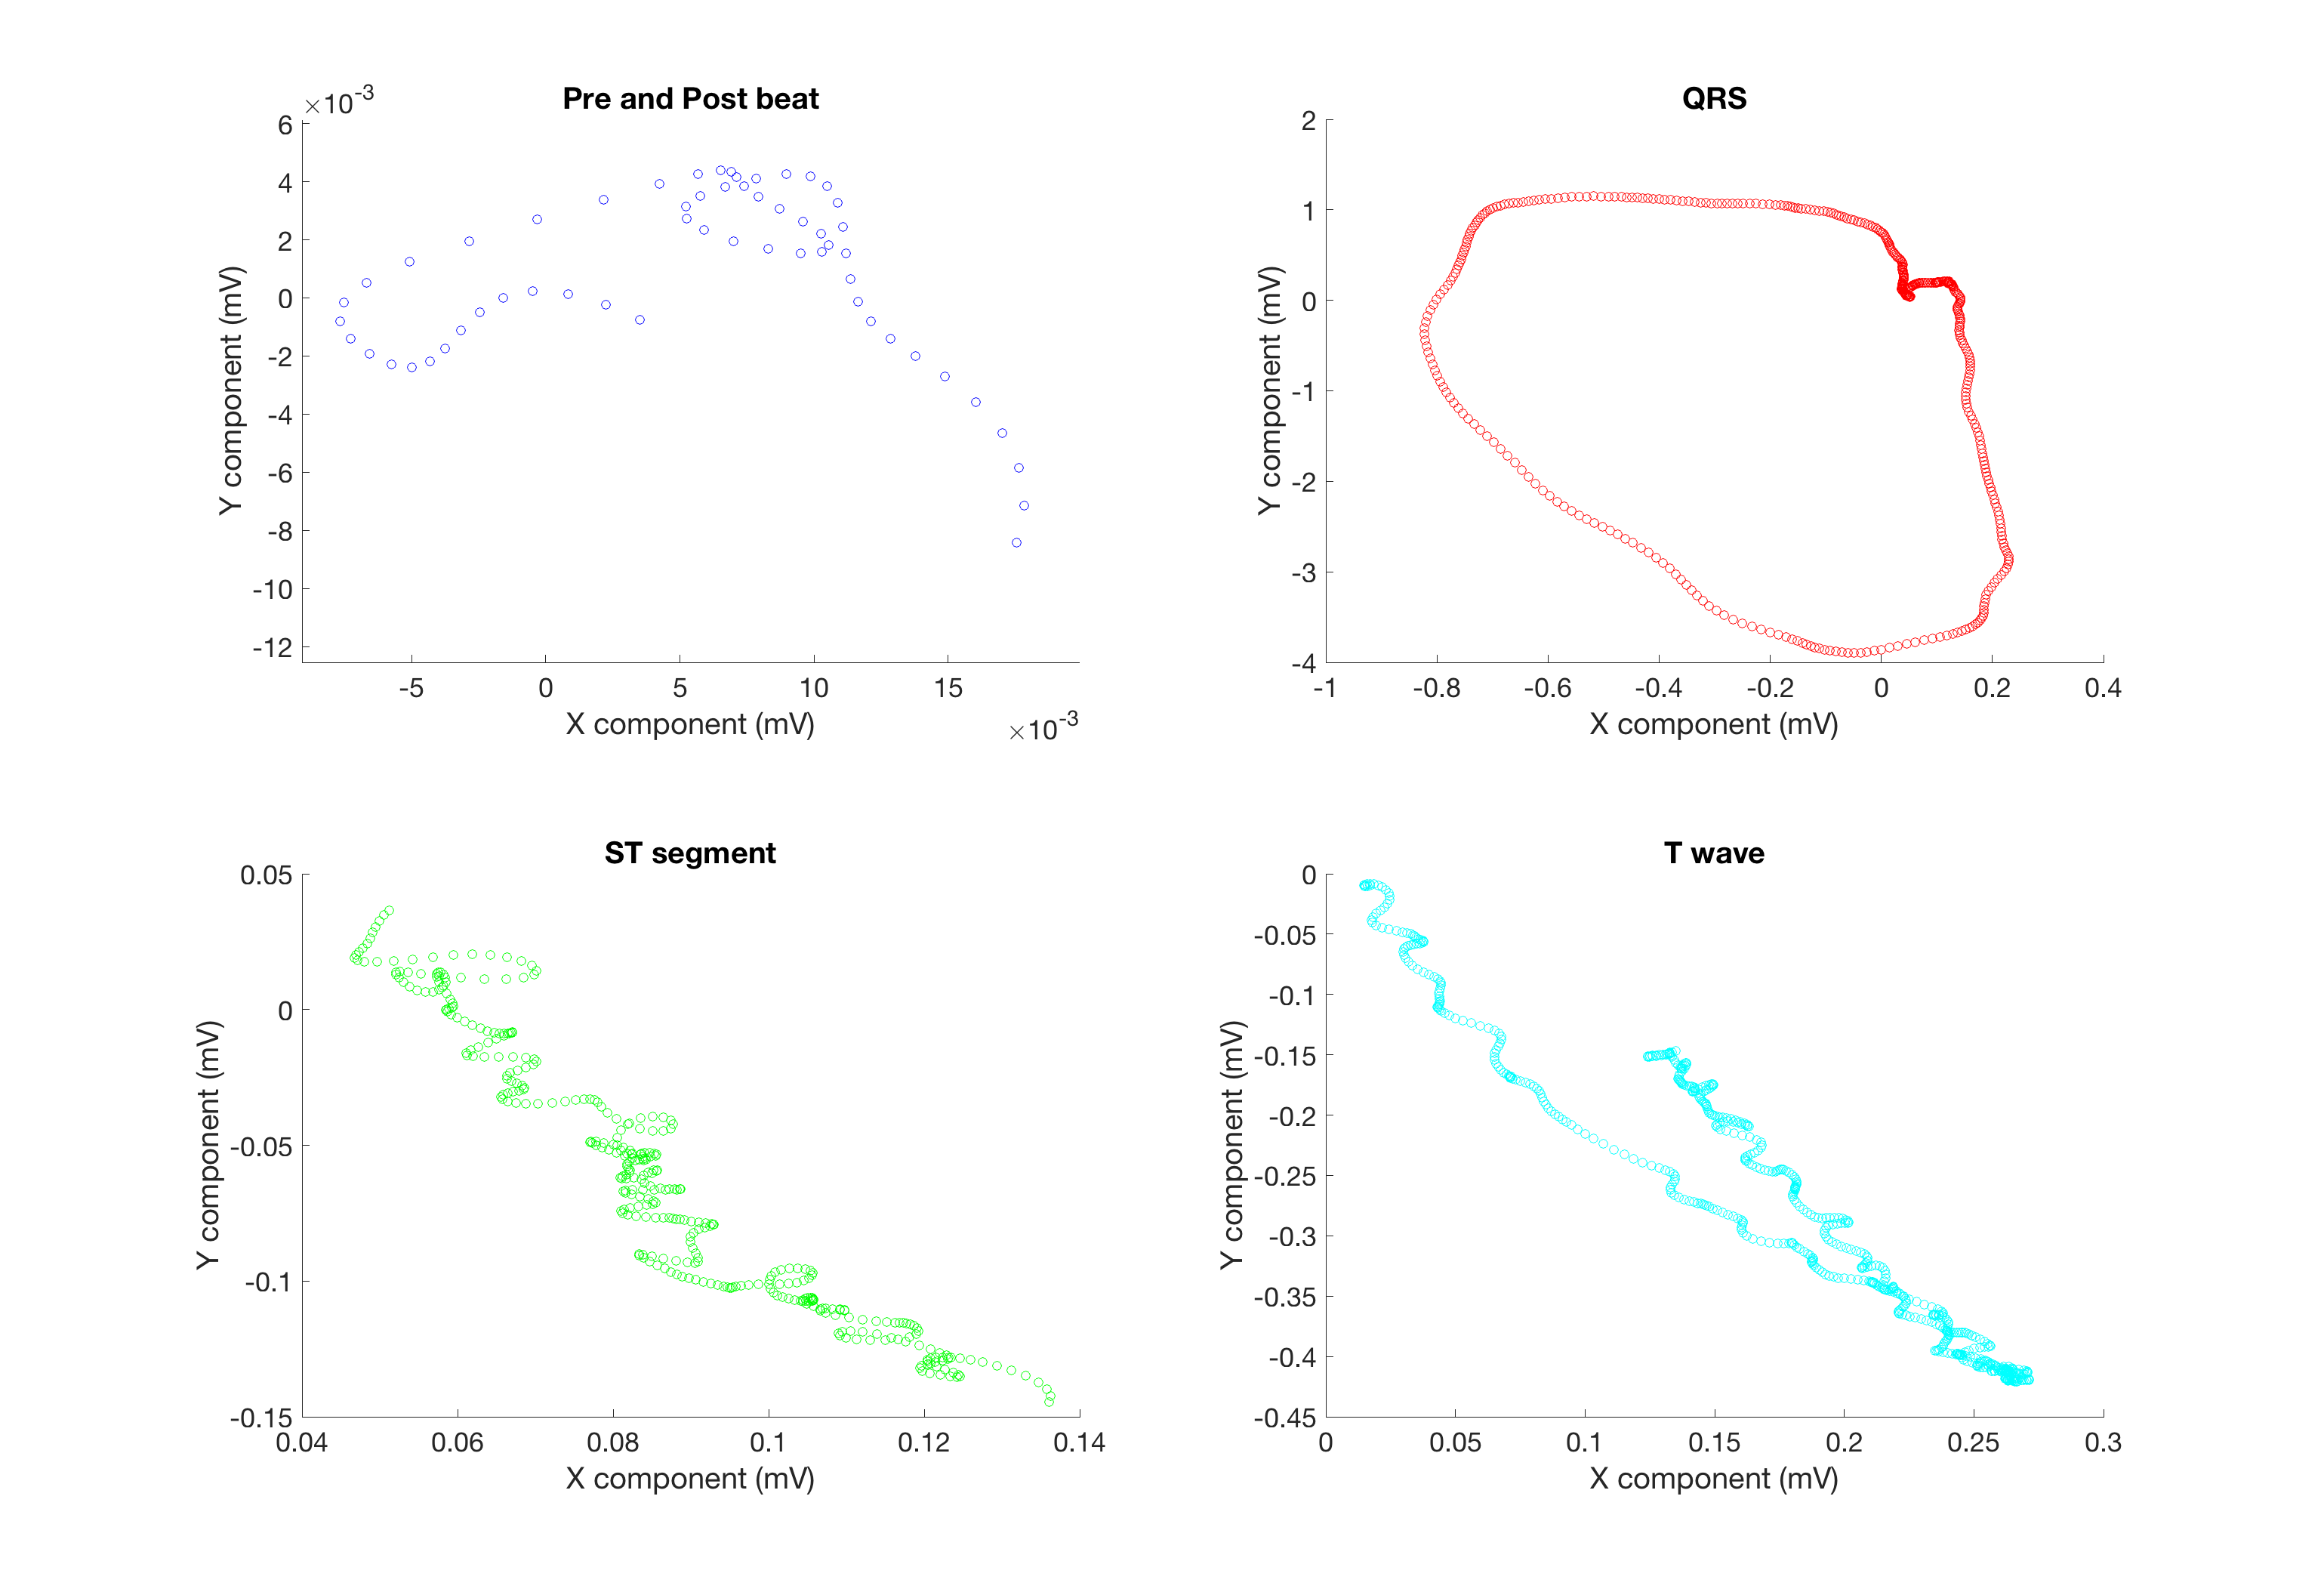
\includegraphics[width = .8\textwidth]{Figures/LimLeads5.png}
	\caption{Separated vectorcardiographs. QRS in Red, ST segment in green, T wave in cyan, isoelectric in blue. }
	\label{fig:Limb5}
\end{figure}

\begin{figure}[H]
	
	\centering
	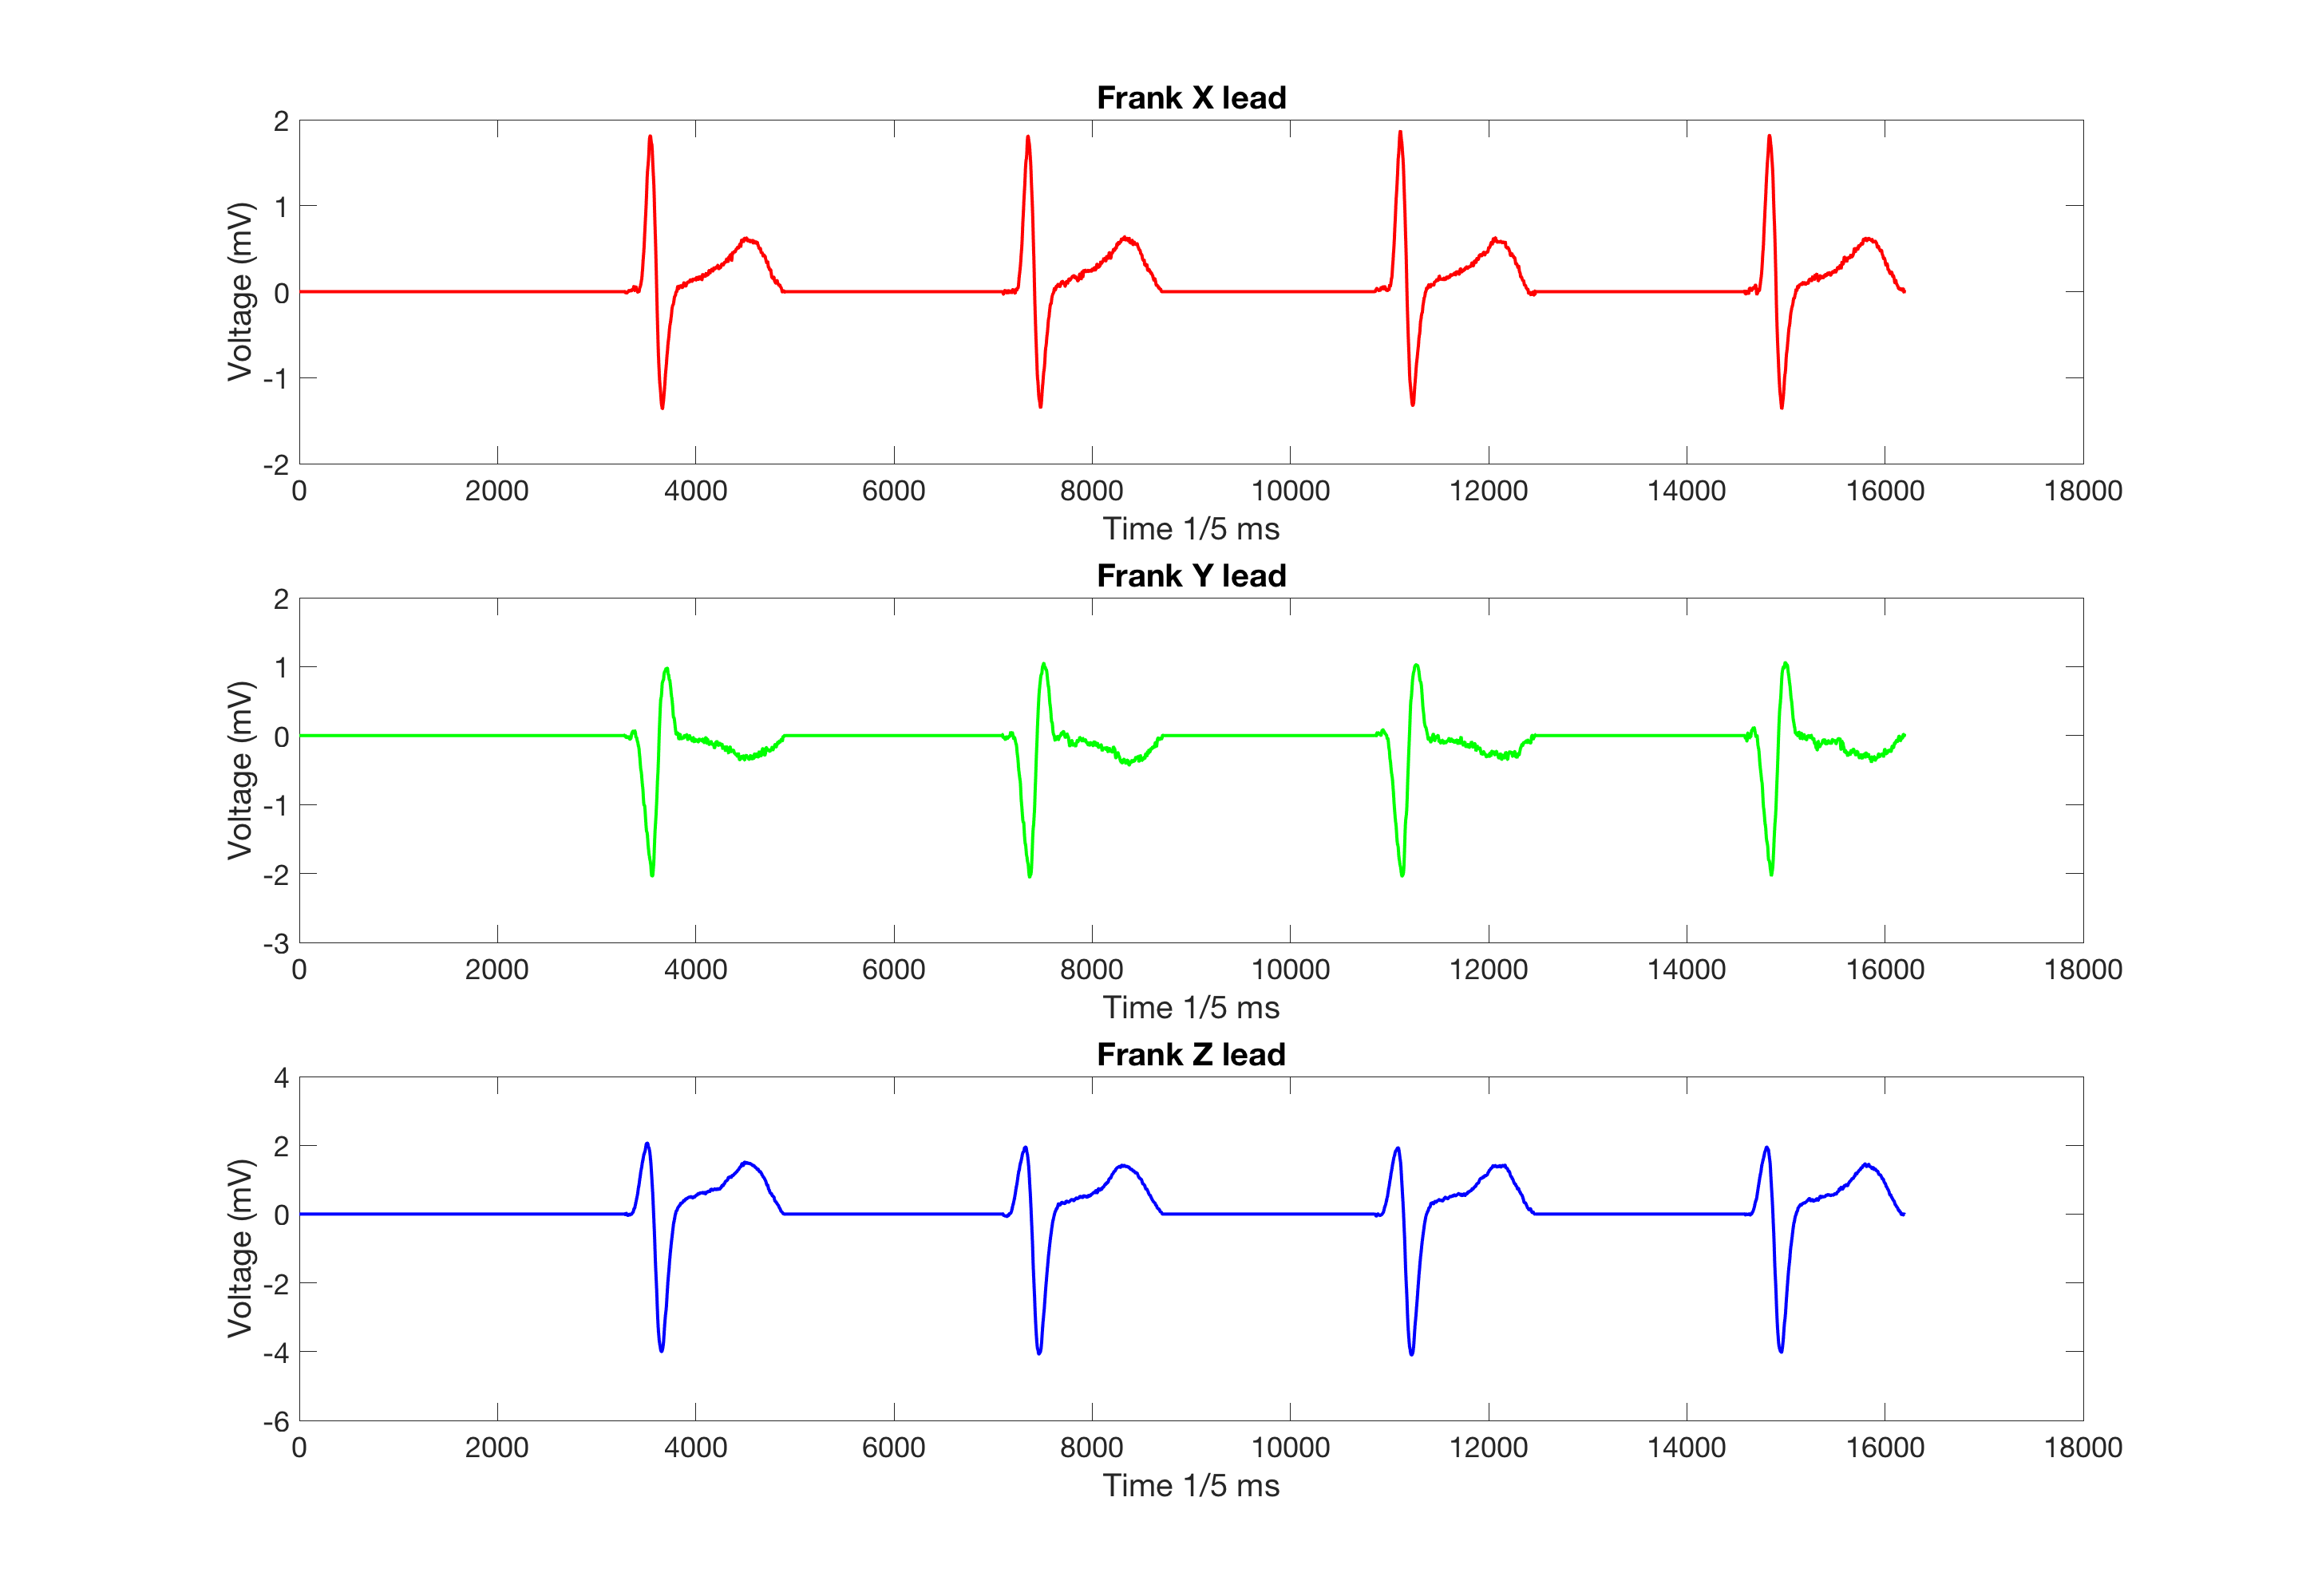
\includegraphics[width = .8\textwidth]{Figures/FrankLeads1.png}
	\caption{ Baseline corrected frank leads. }
	\label{fig:Frank1}
\end{figure}

\begin{figure}[H]
	
	\centering
	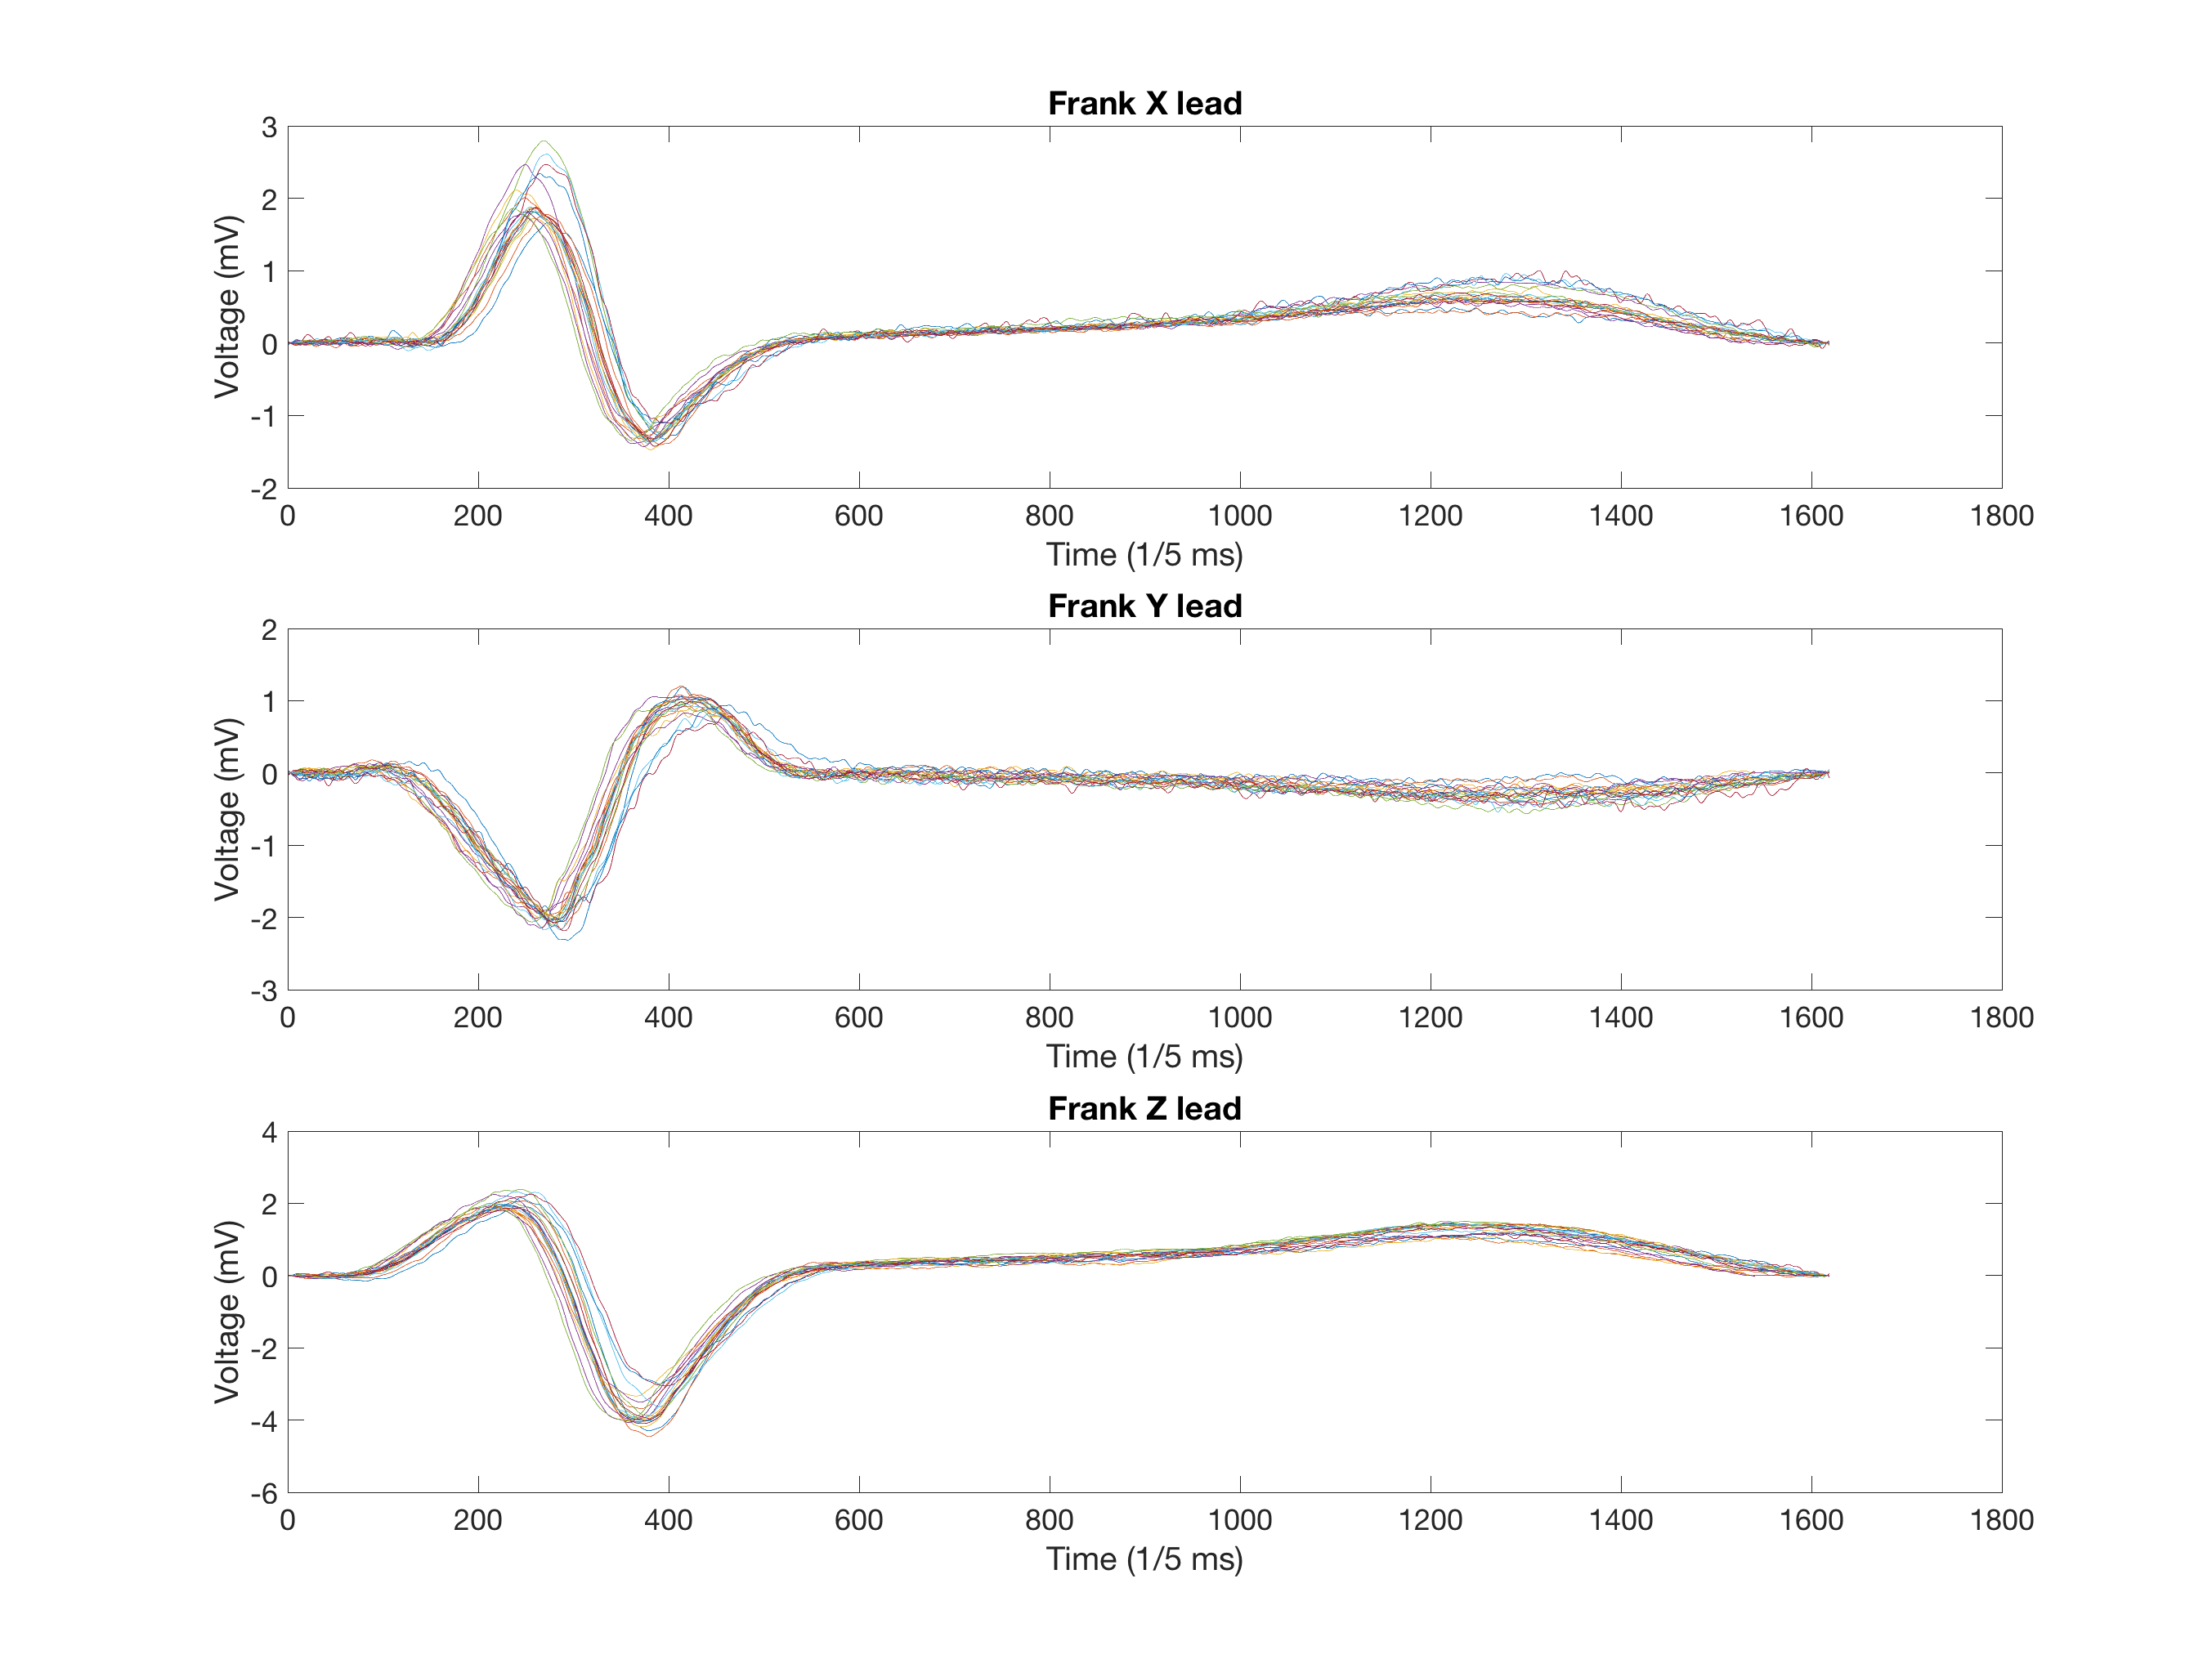
\includegraphics[width = .8\textwidth]{Figures/FrankLeads2.png}
	\caption{ Several autofiducilized beats from the frank leads.}
	\label{fig:Frank2}
\end{figure}

\begin{figure}[H]
	
	\centering
	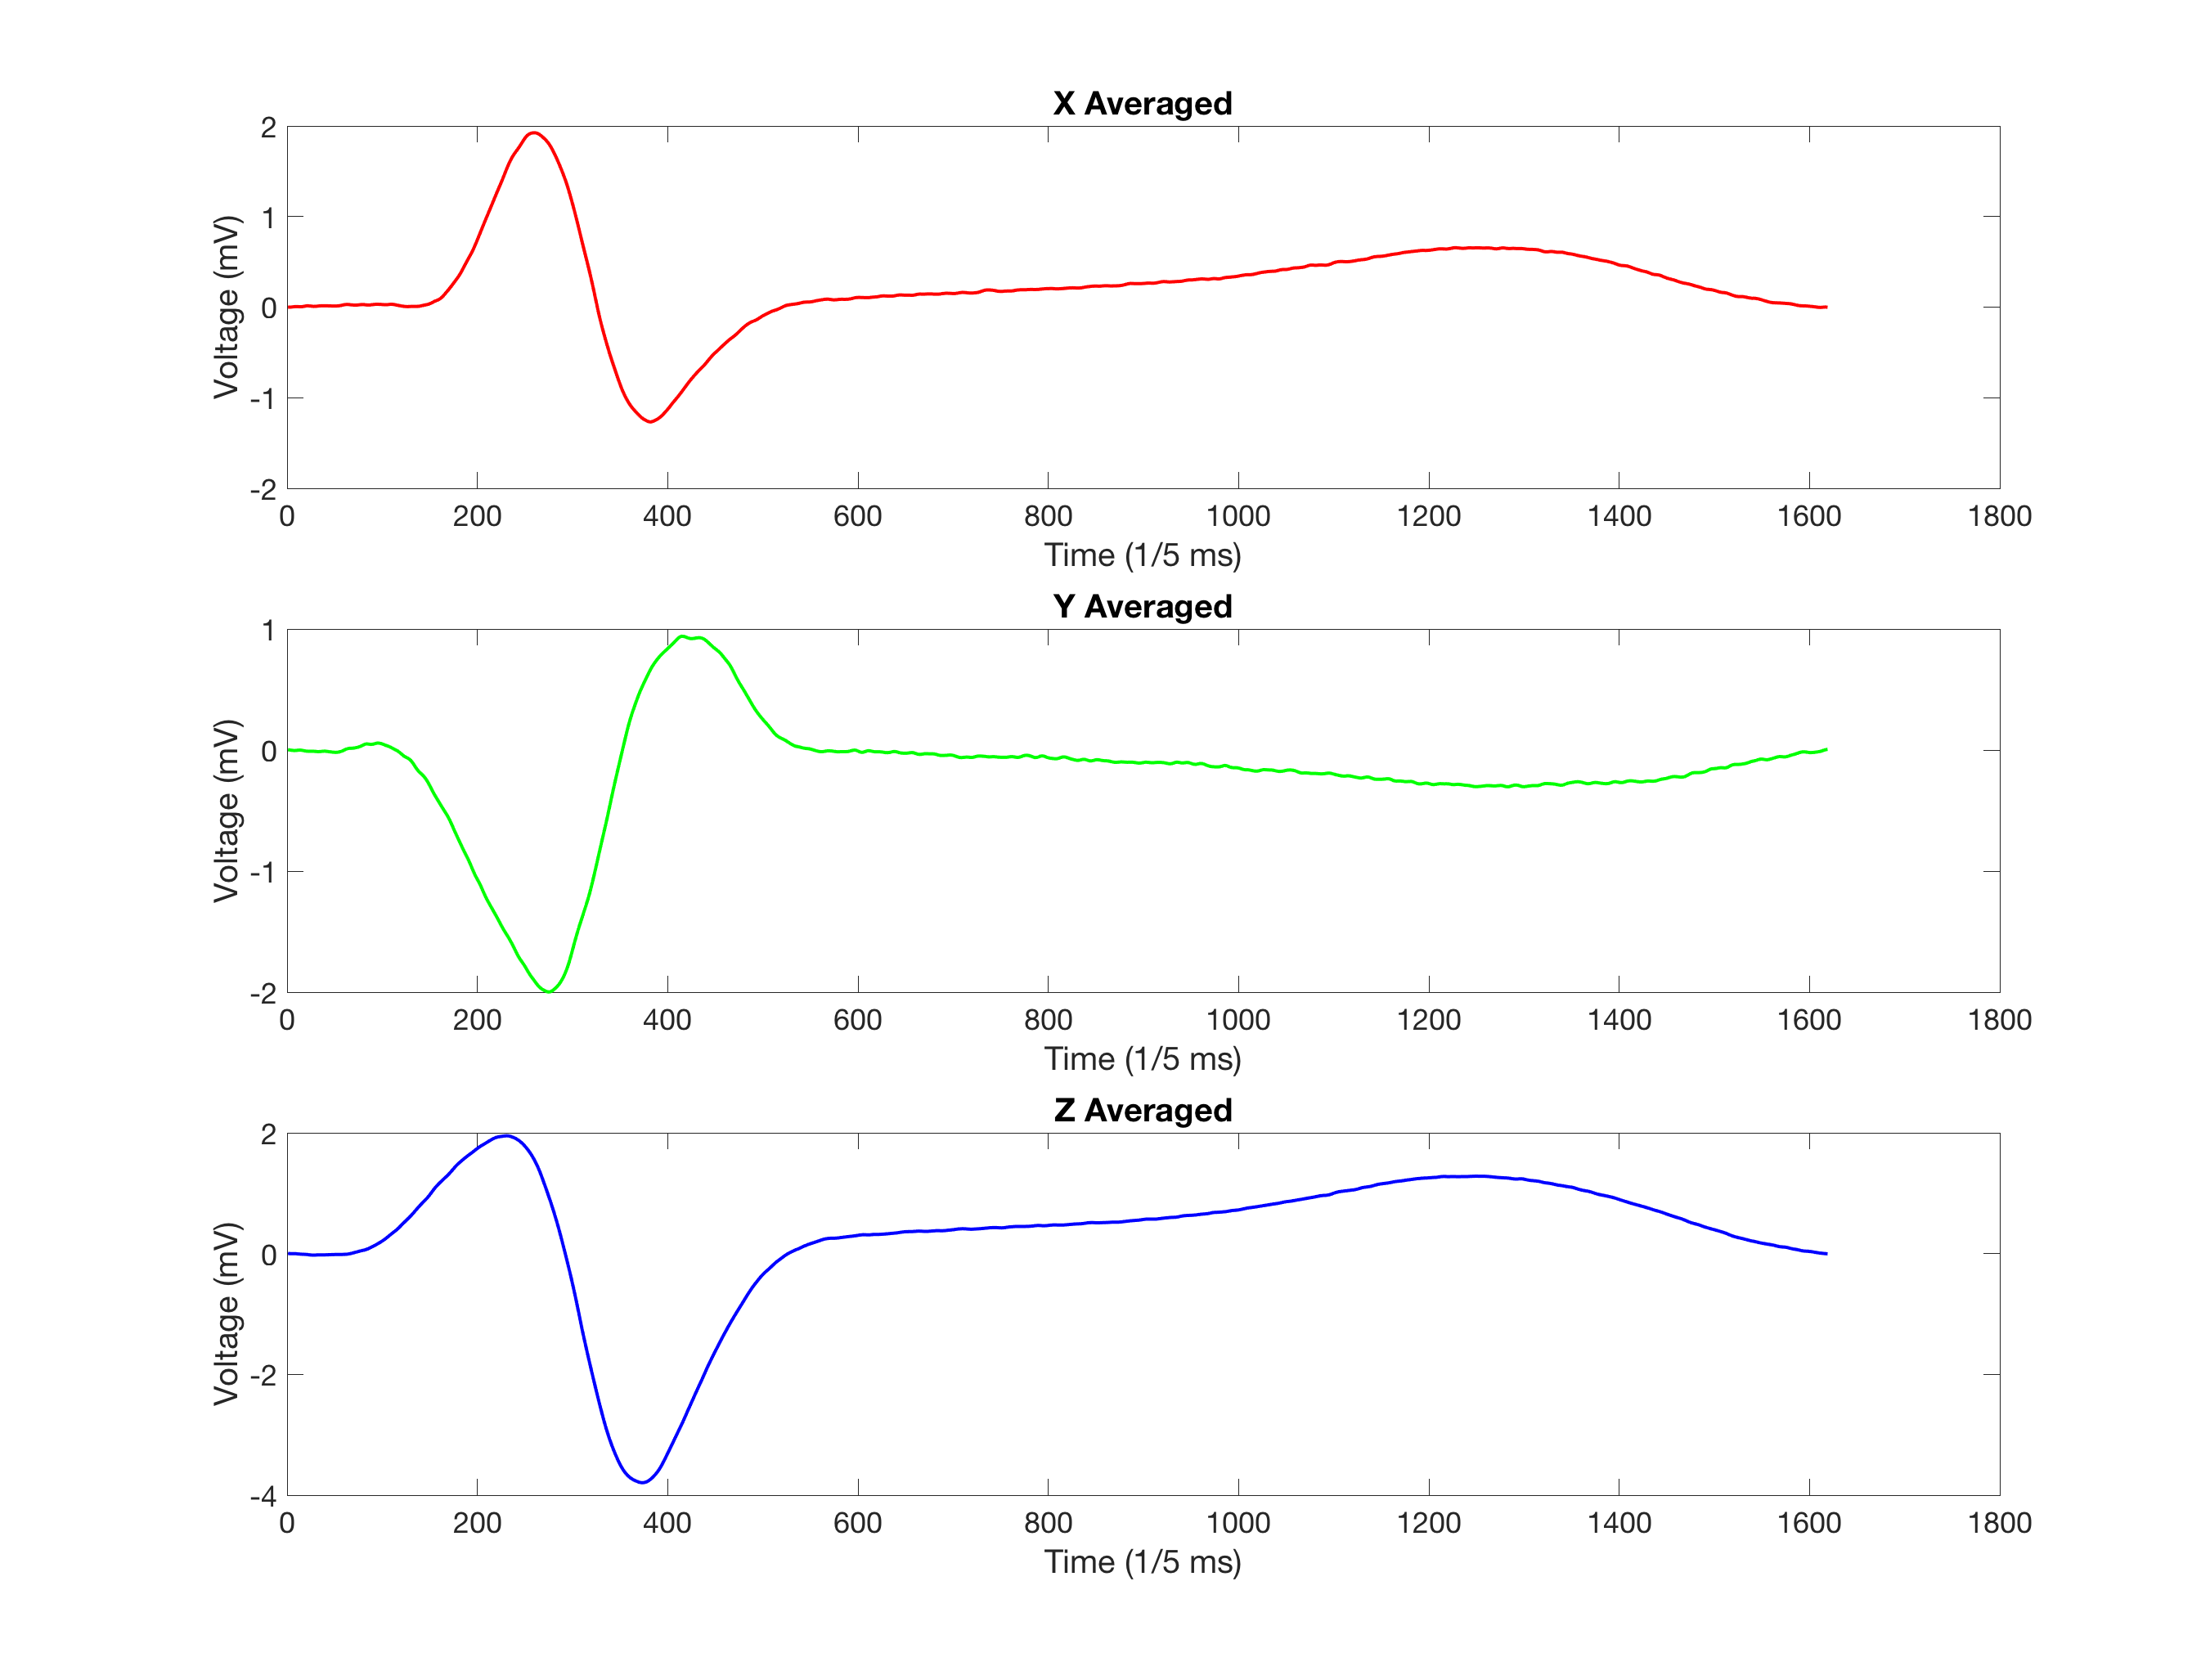
\includegraphics[width = .8\textwidth]{Figures/FrankLeads3.png}
	\caption{Signal averaged frank leads.}
	\label{fig:Frank3}
\end{figure}

\begin{figure}[H]
	
	\centering
	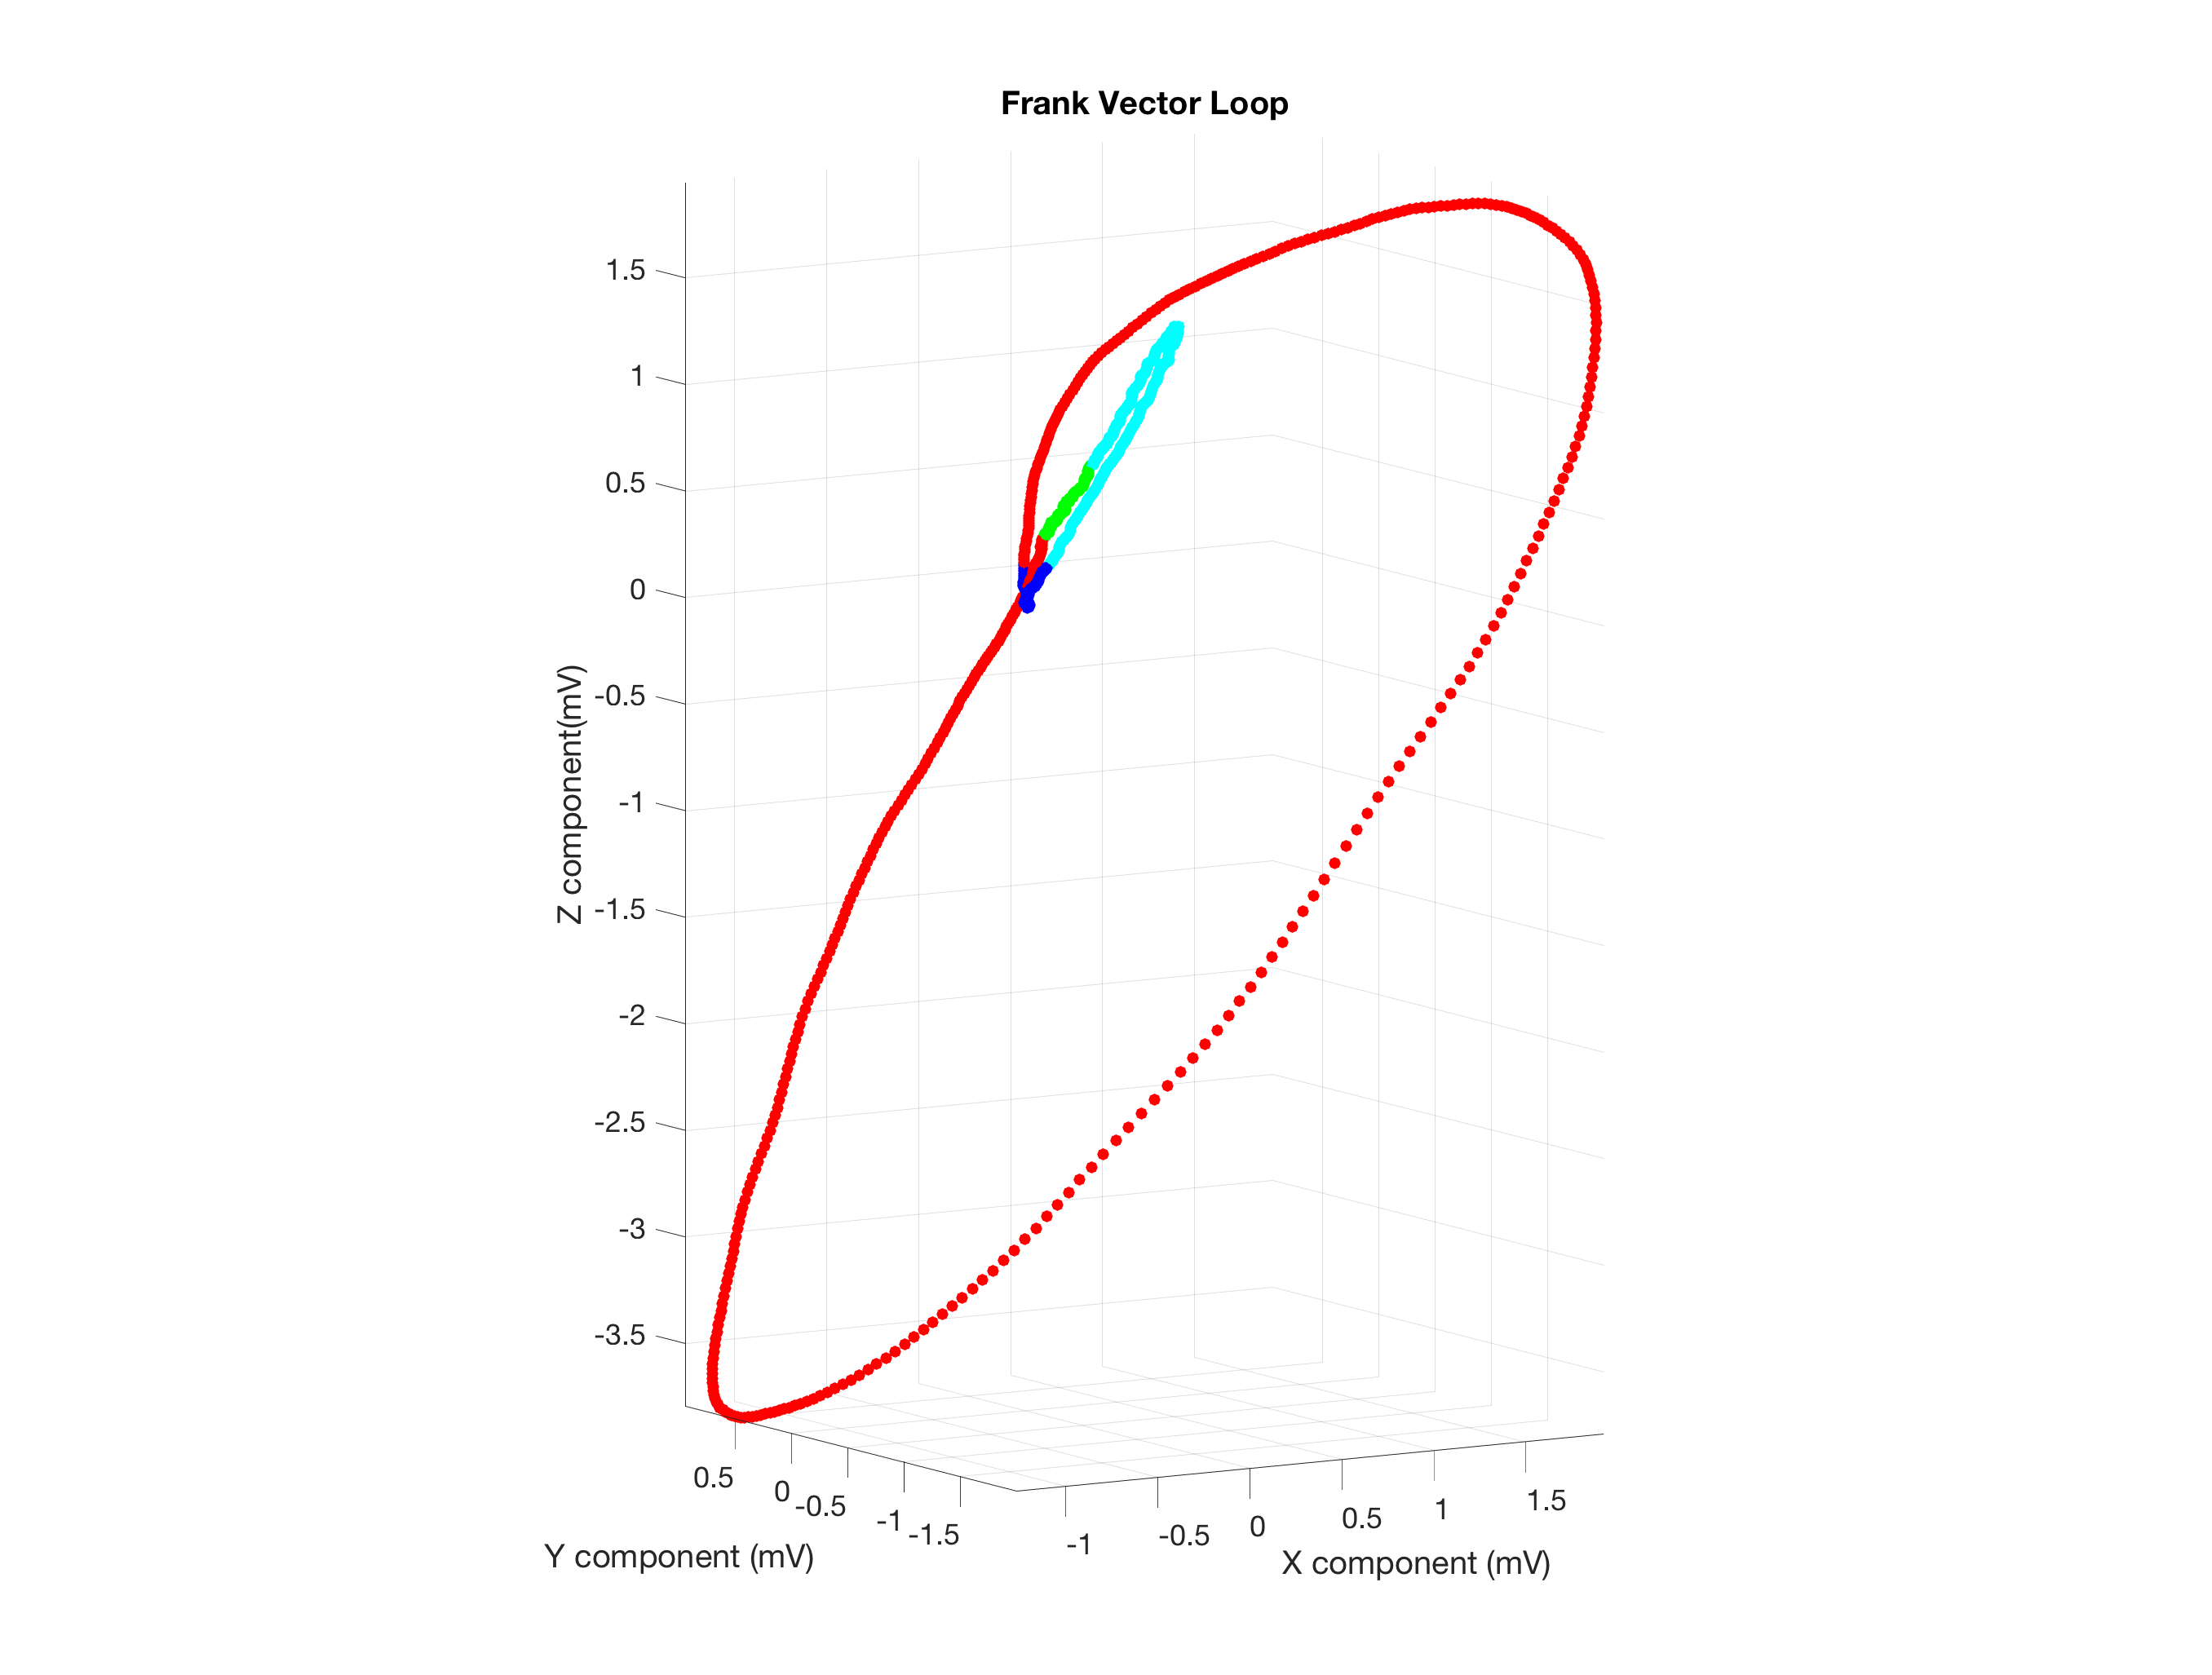
\includegraphics[width = .7\textwidth]{Figures/FrankLeads_3d.png}
	\caption{Frank lead vector cardiograph in 3D. QRS in Red, ST segment in green, T wave in cyan, isoelectric in blue.}
	\label{fig:Frank3D}
\end{figure}

\begin{figure}[H]
	
	\centering
	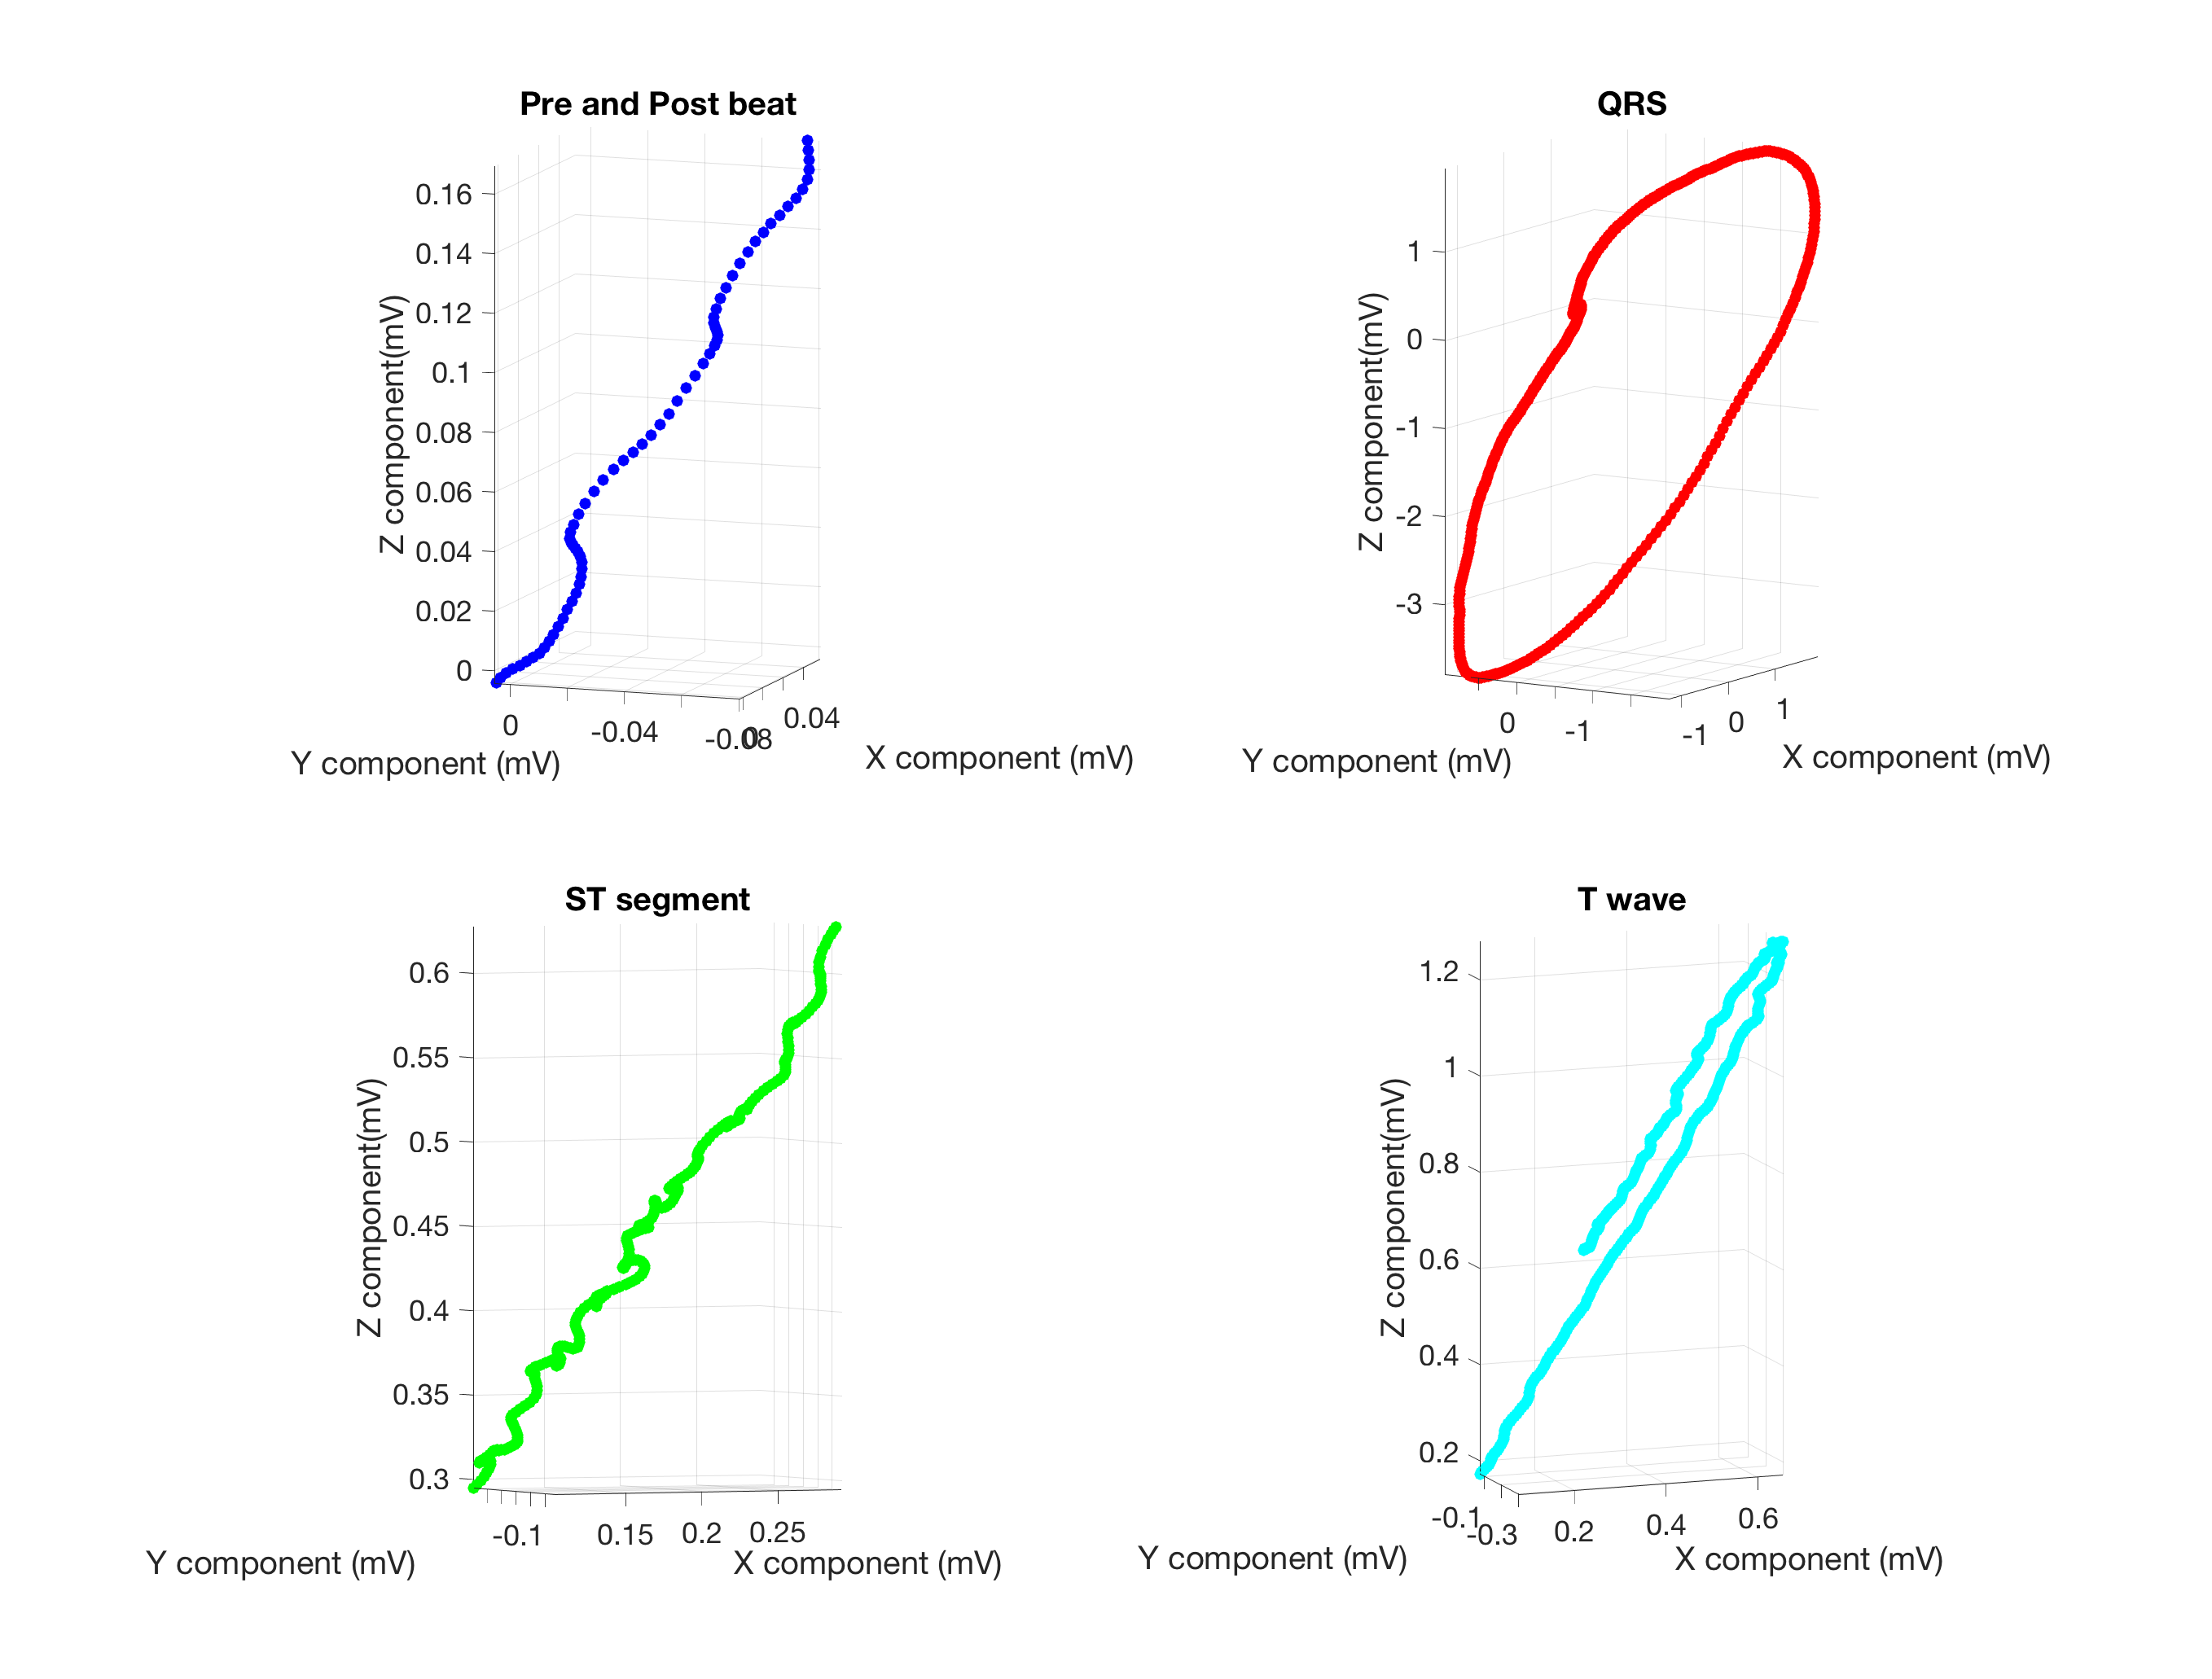
\includegraphics[width = .75\textwidth]{Figures/FrankLeads_3d_split.png}
	\caption{Frank lead vector cardiograph in 3D split by segment. QRS in Red, ST segment in green, T wave in cyan, isoelectric in blue.}
	\label{fig:Frank3D_split}
\end{figure}

\begin{figure}[H]
	
	\centering
	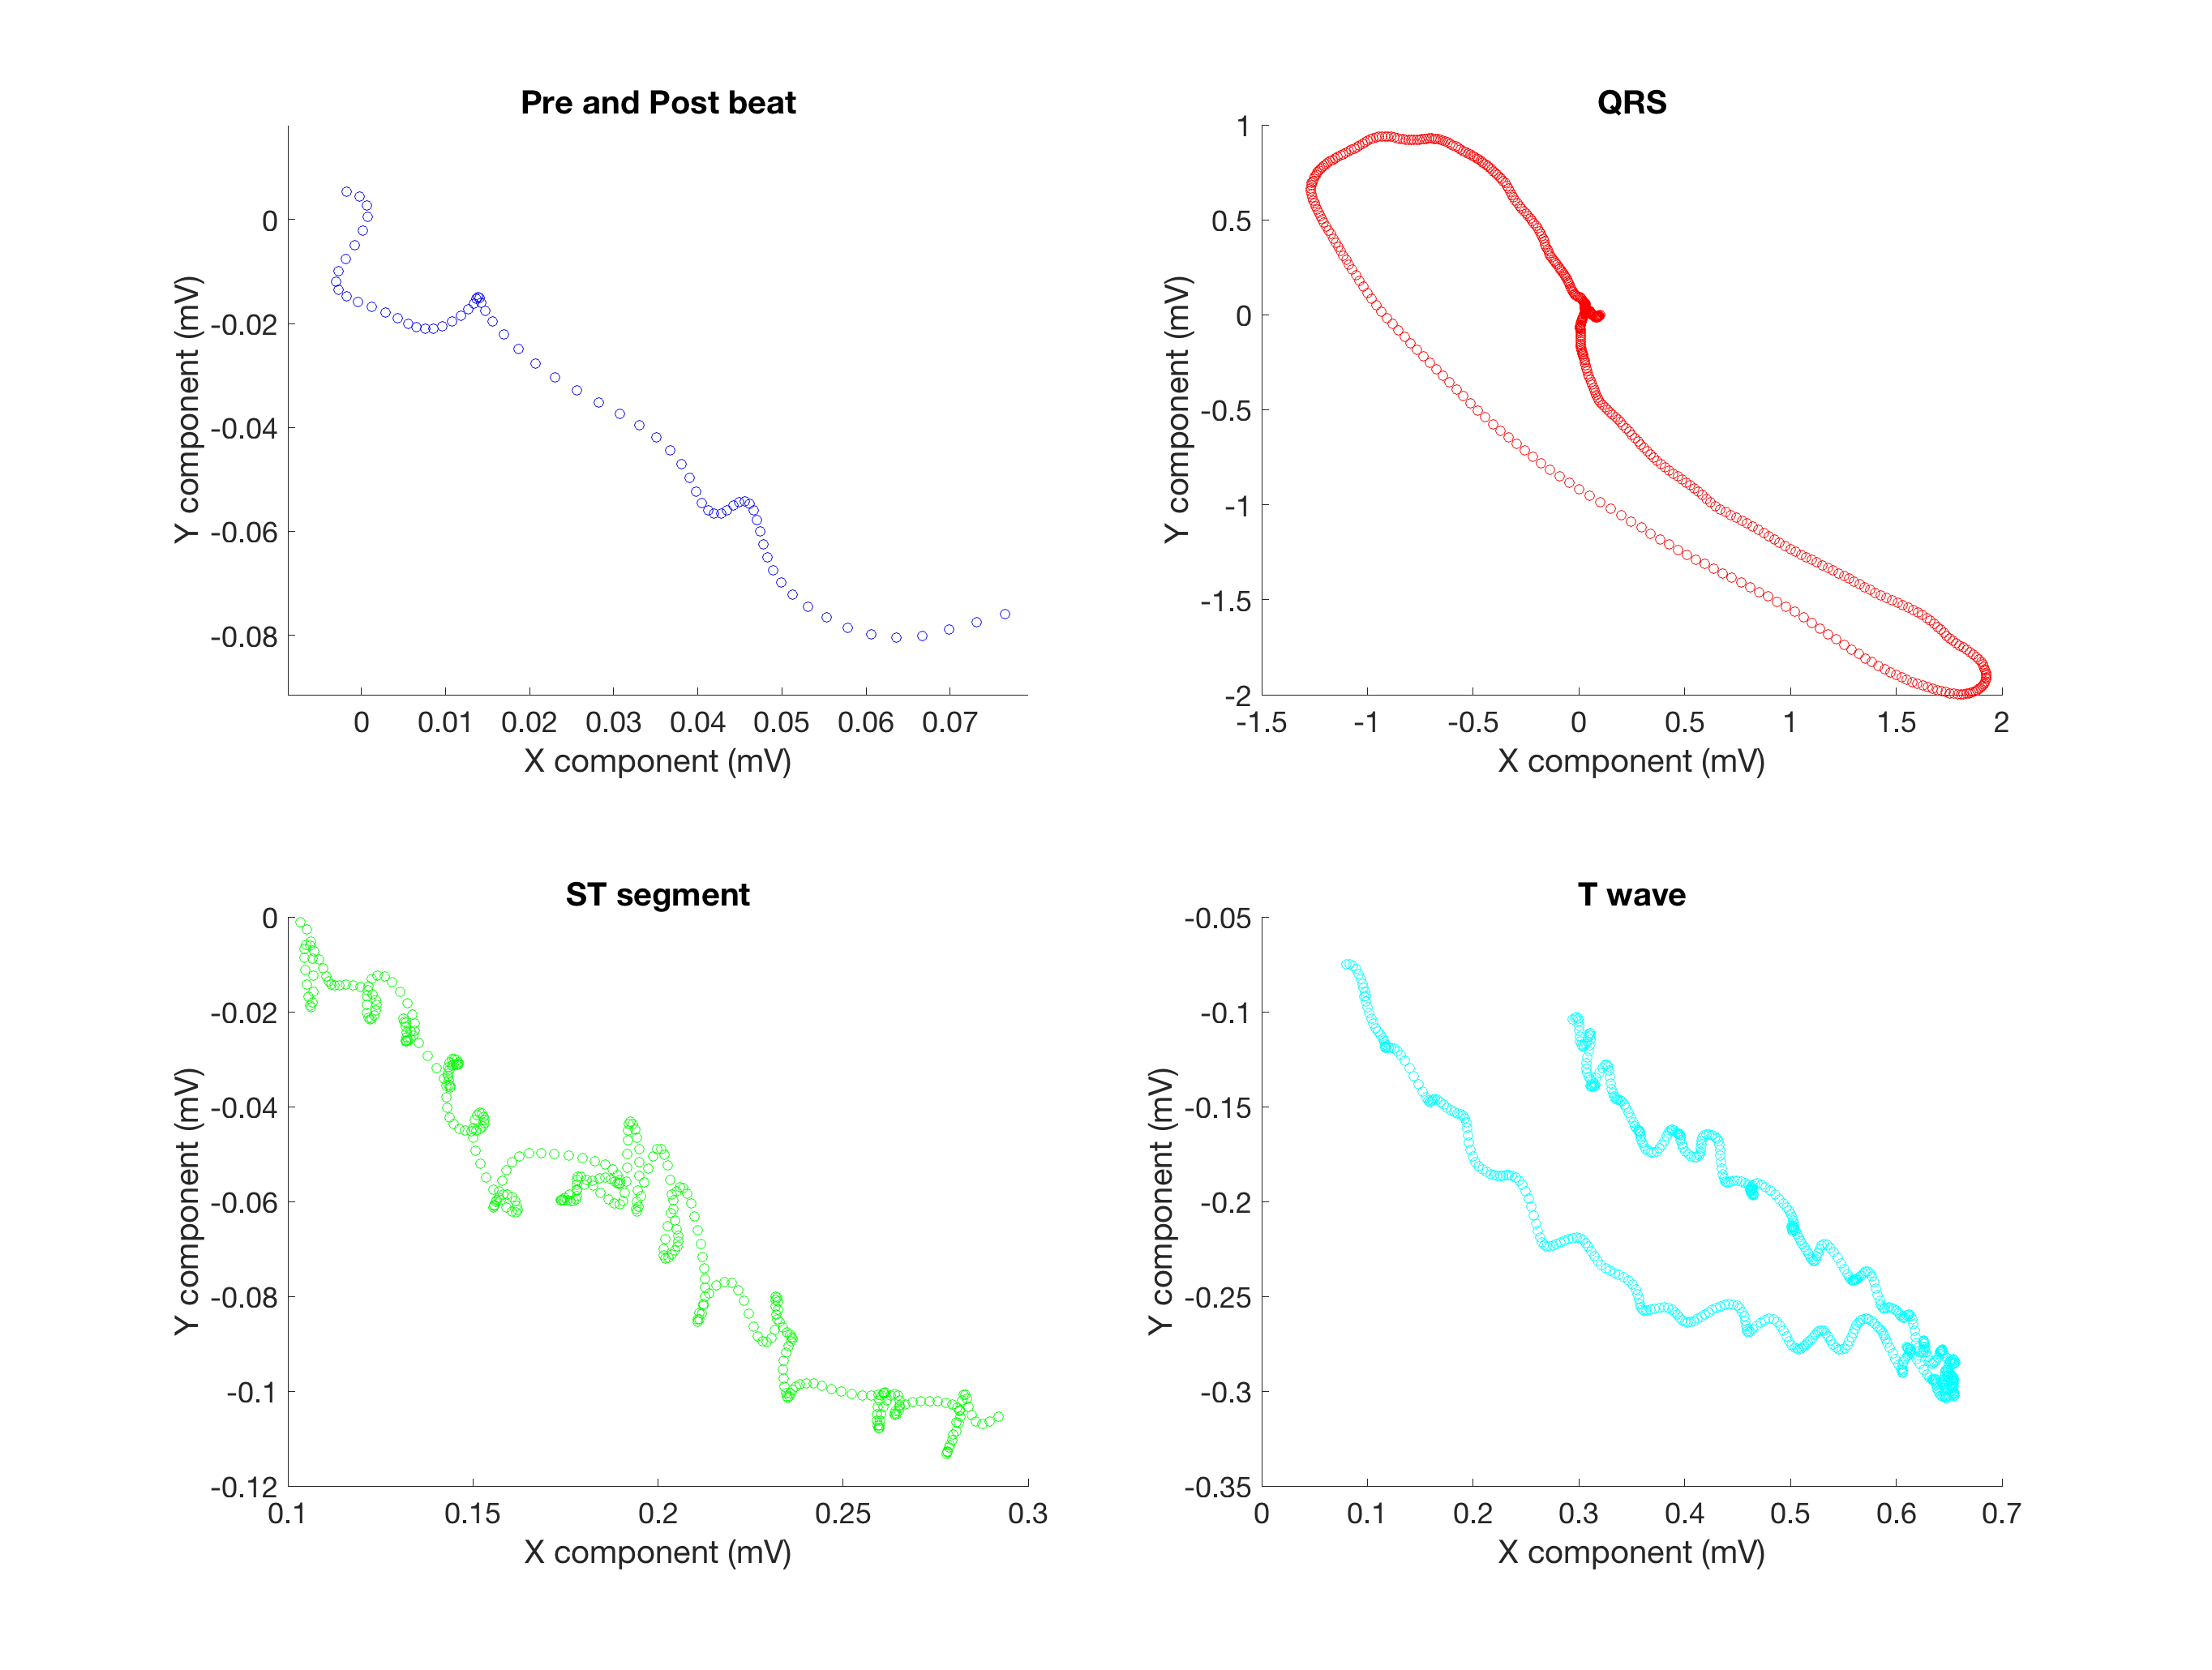
\includegraphics[width = .75\textwidth]{Figures/FrankLeads_xy.png}
	\caption{Frank lead vector cardiograph in the X-Y frontal plane. QRS in Red, ST segment in green, T wave in cyan, isoelectric in blue. }
	\label{fig:Frank_xy}
\end{figure}

\begin{figure}[H]
	
	\centering
	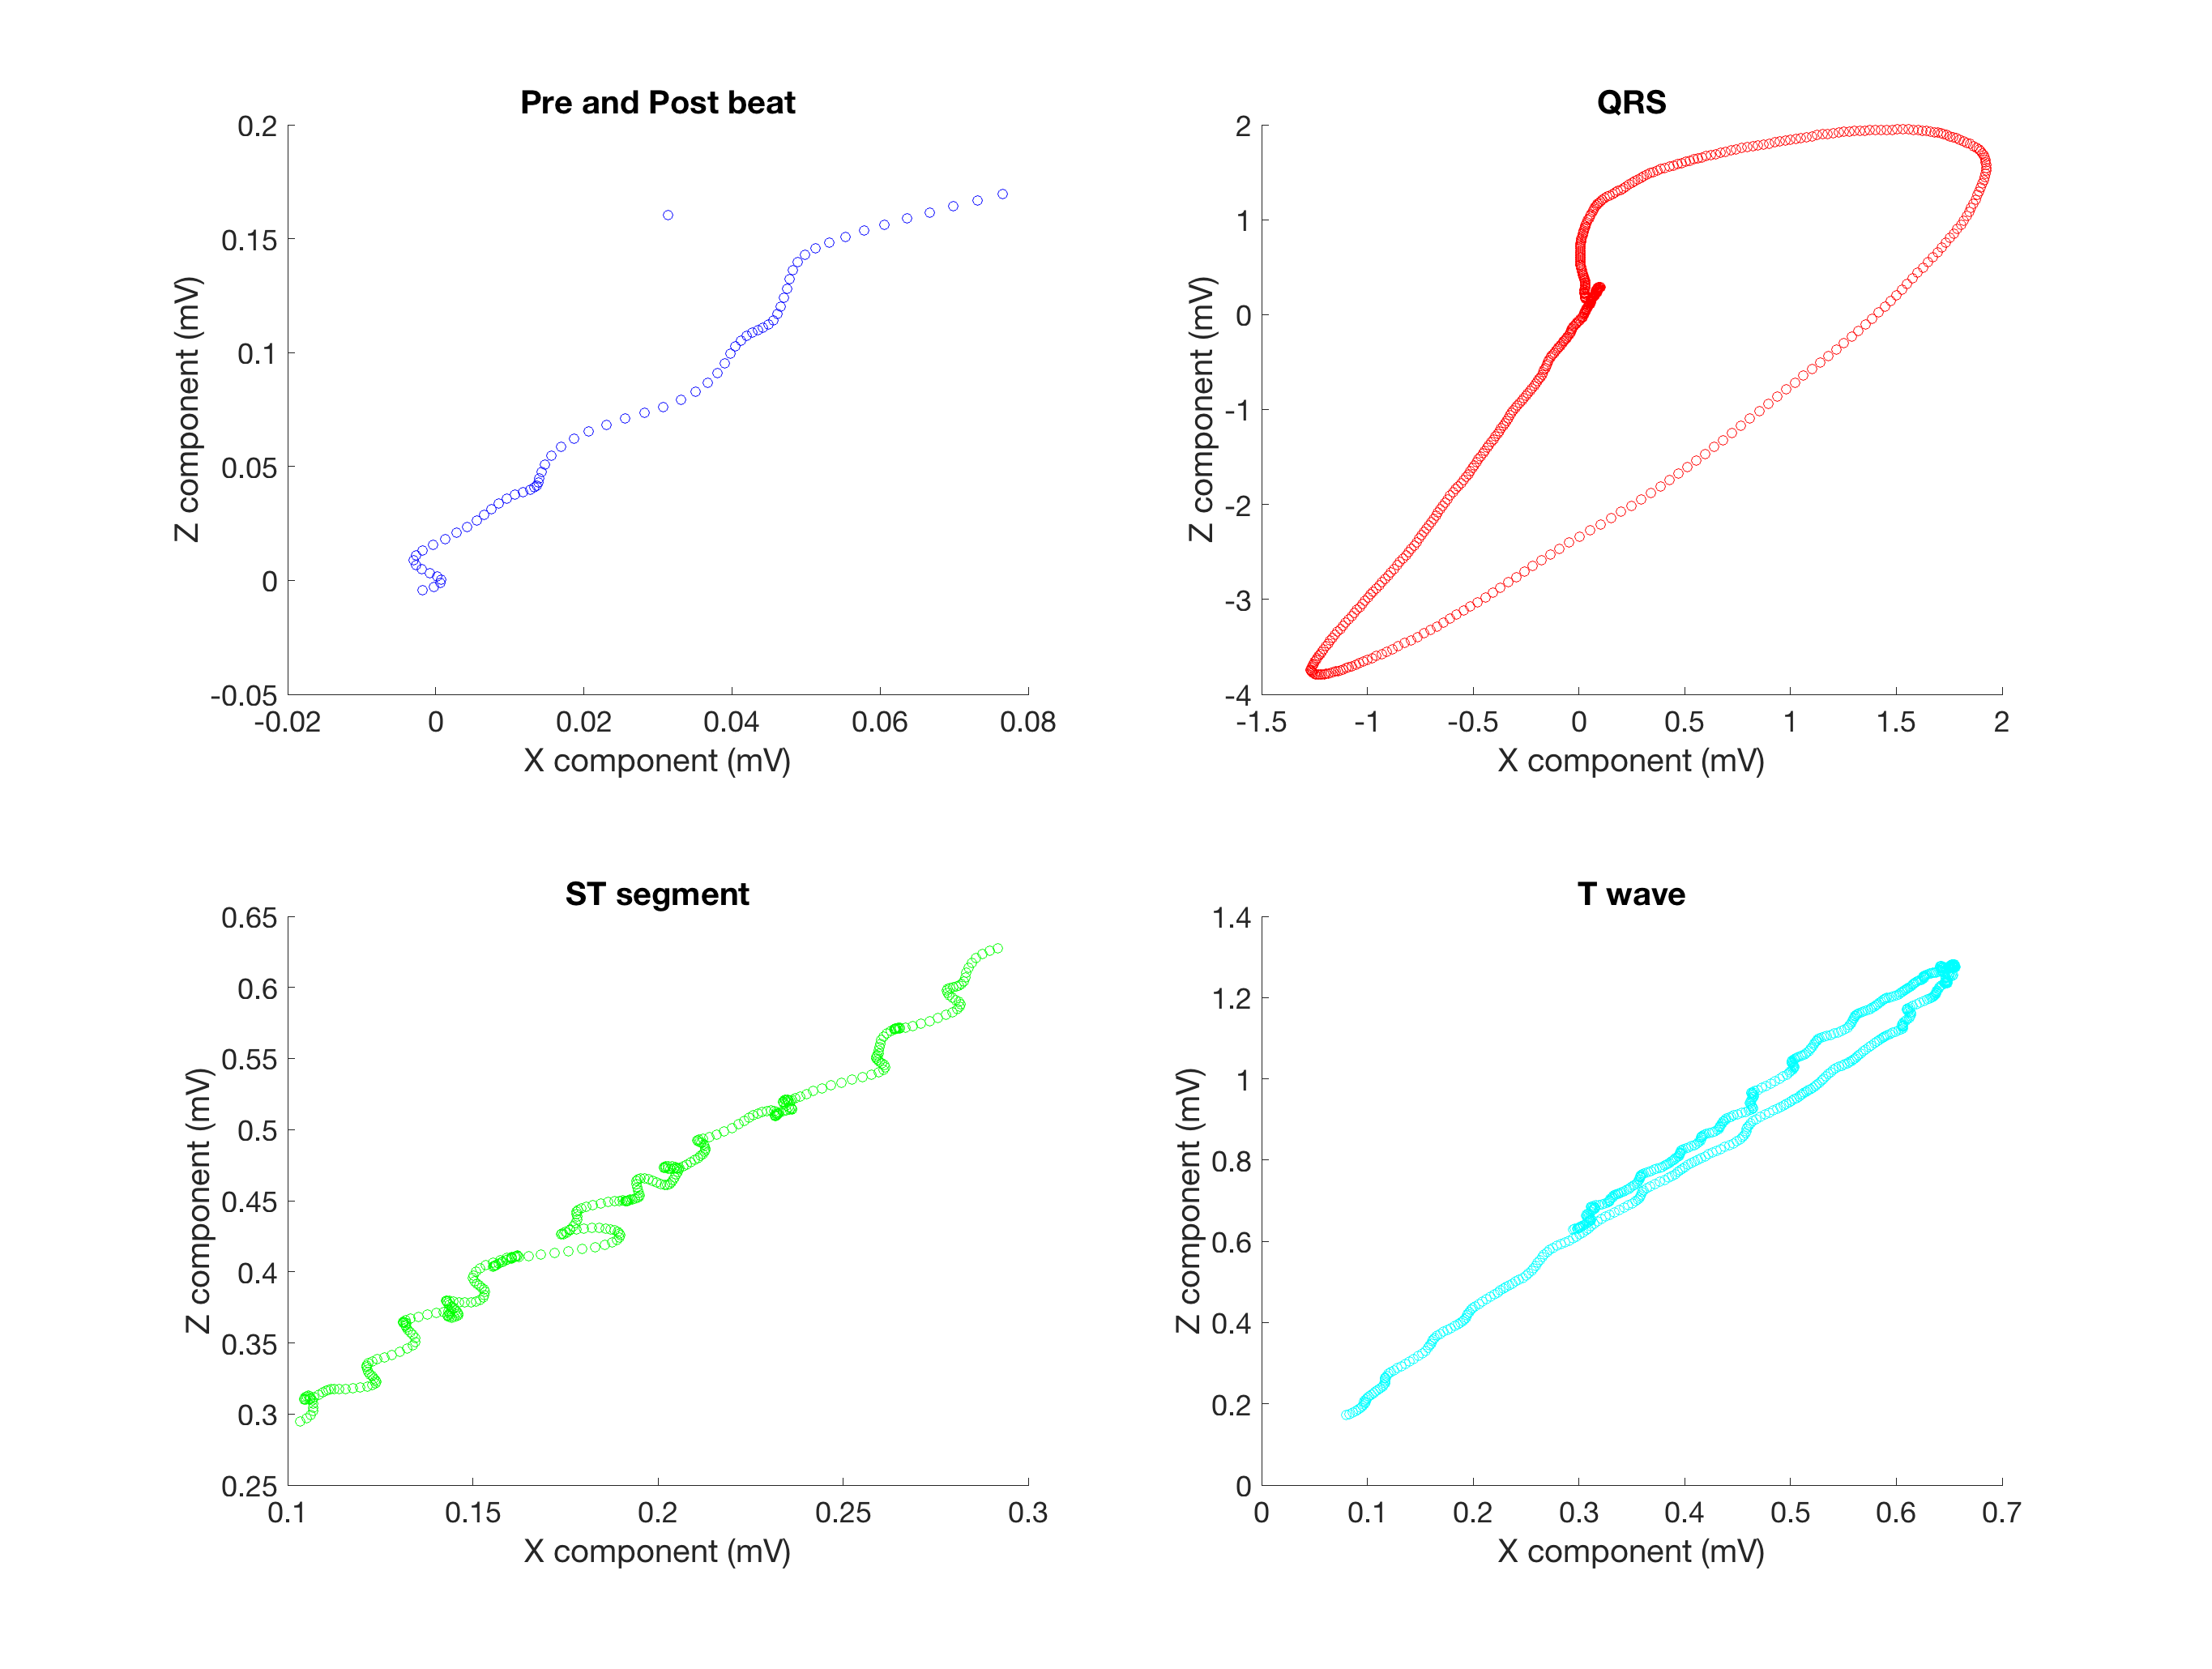
\includegraphics[width = .75\textwidth]{Figures/FrankLeads_xz.png}
	\caption{ Frank lead vector cardiograph in the X-Z coronal plane. QRS in Red, ST segment in green, T wave in cyan, isoelectric in blue.}
	\label{fig:Frank_xz}
\end{figure}

\begin{figure}[H]
	
	\centering
	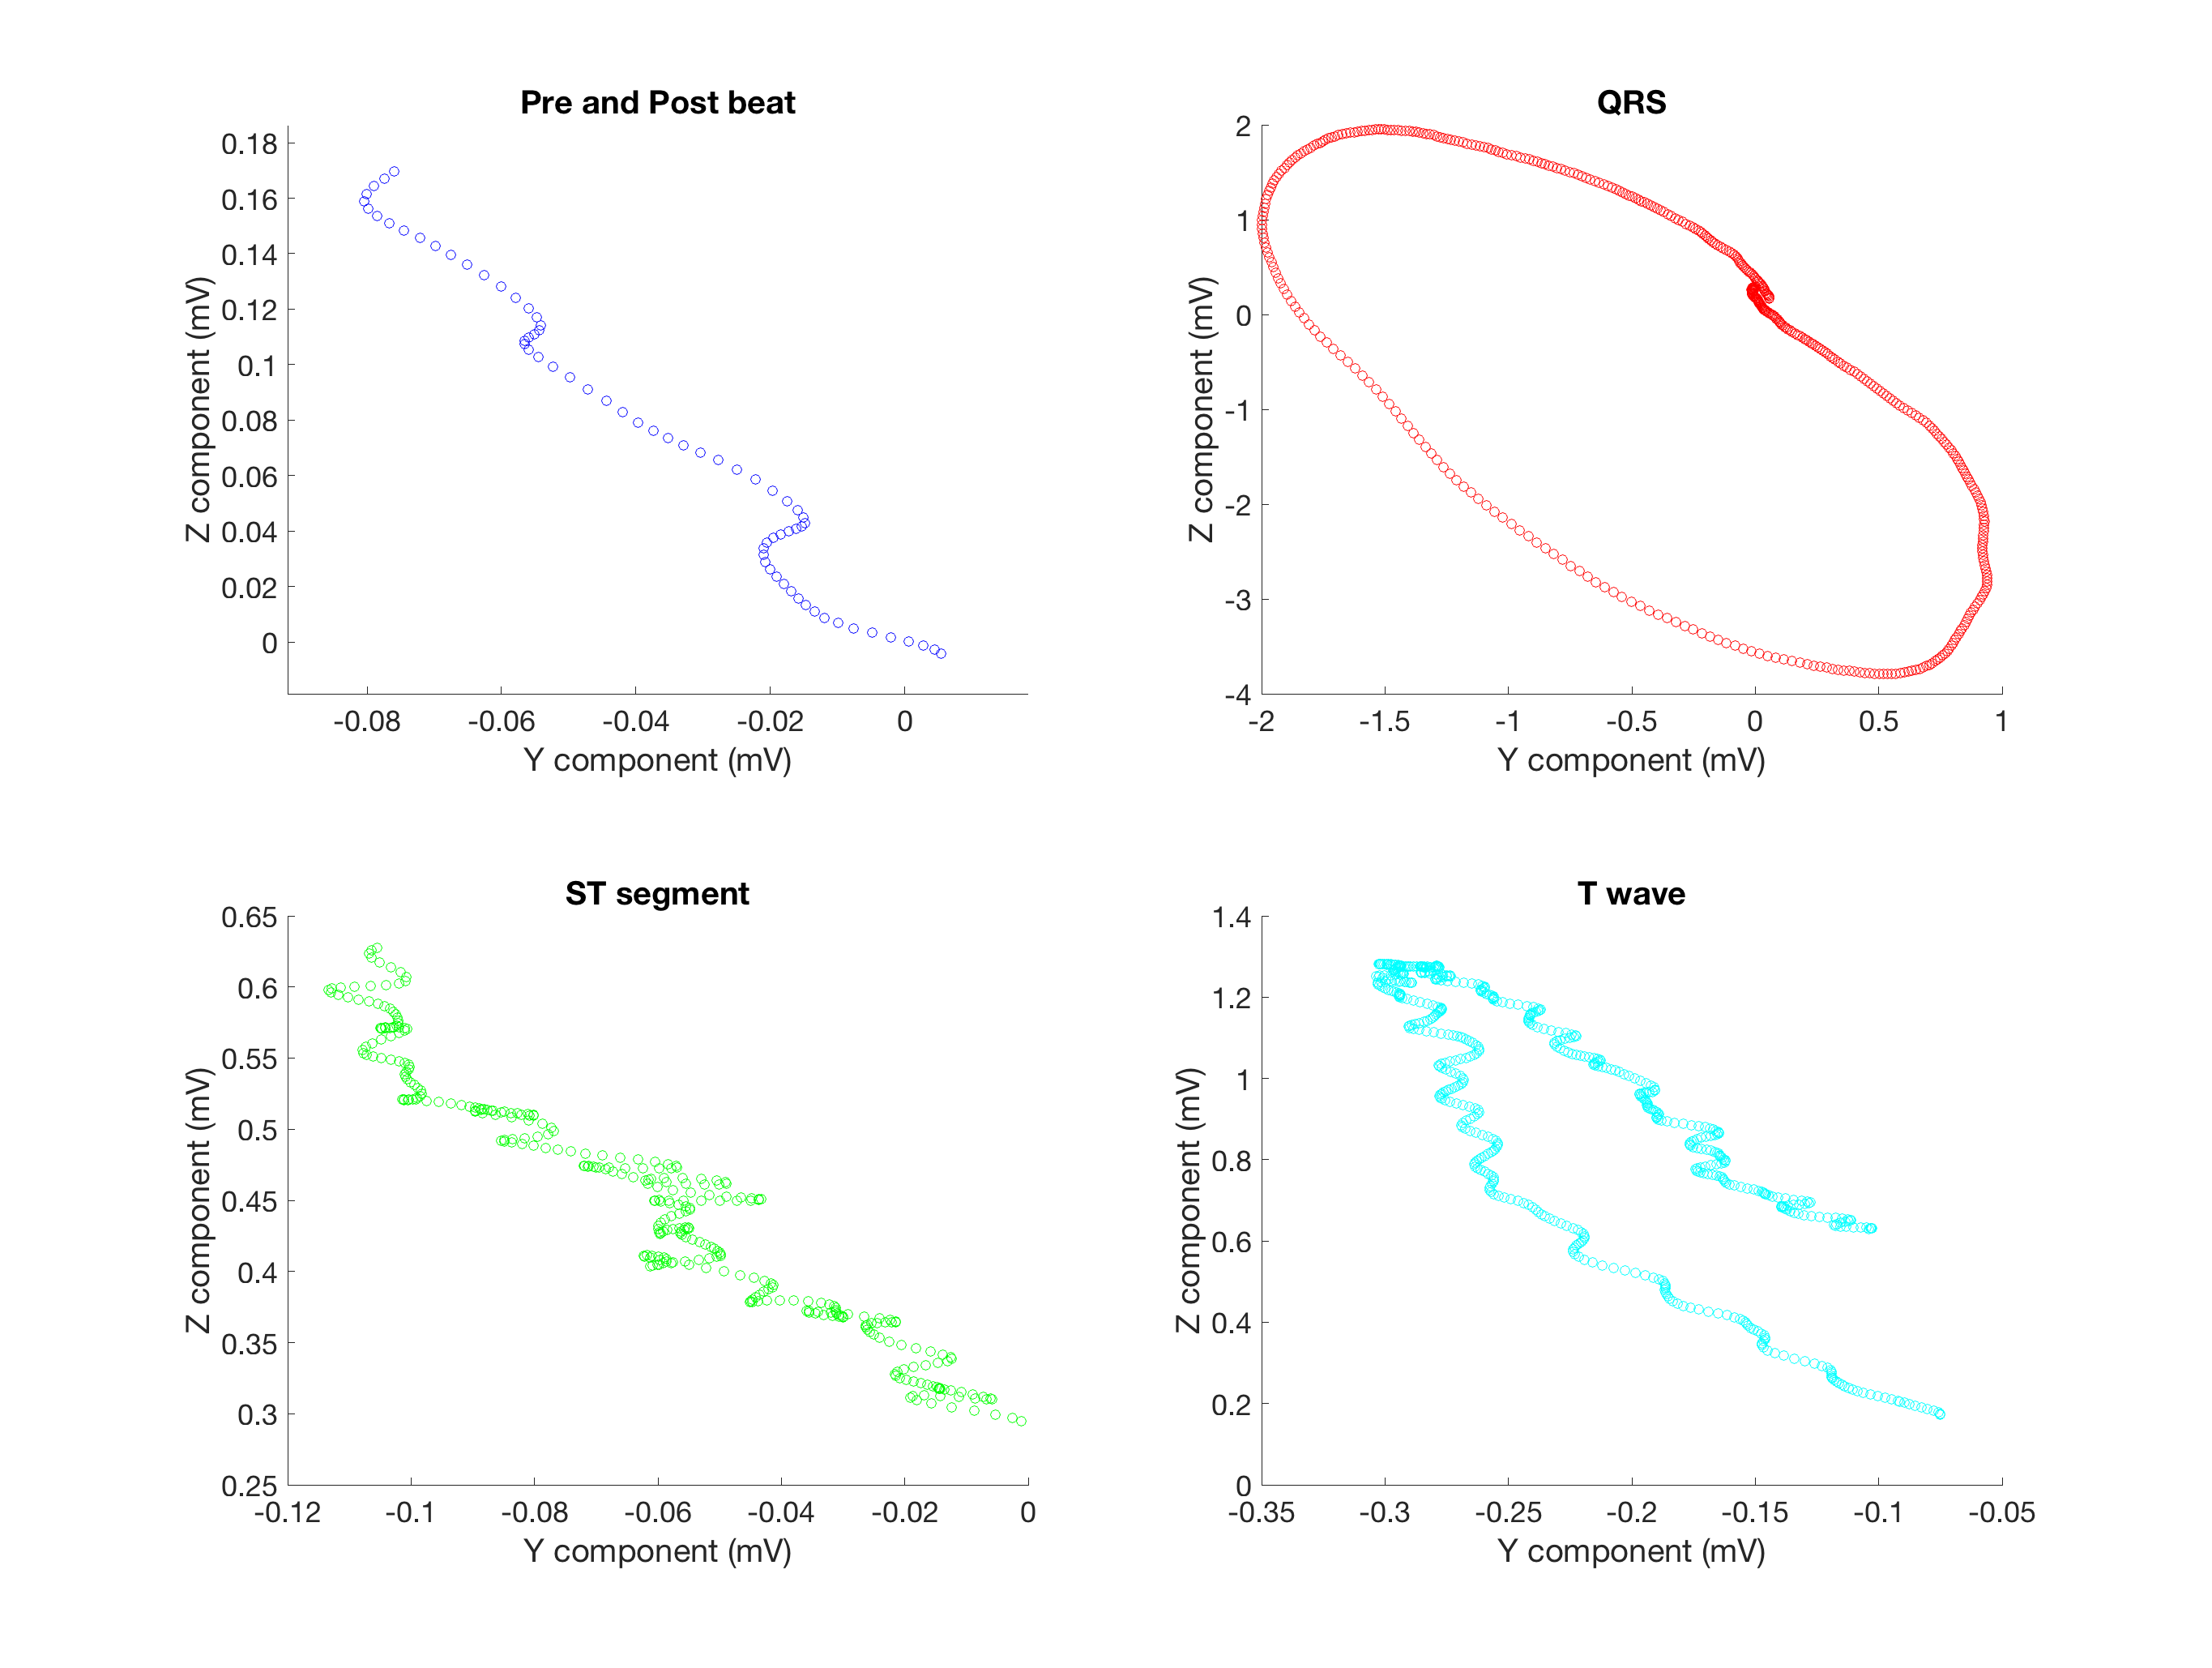
\includegraphics[width = .75\textwidth]{Figures/FrankLeads_yz.png}
	\caption{ Frank lead vector cardiograph in the Y-Z sagital plane. QRS in Red, ST segment in green, T wave in cyan, isoelectric in blue.}
	\label{fig:Frank_yz}
\end{figure}

\begin{figure}[H]
	
	\centering
	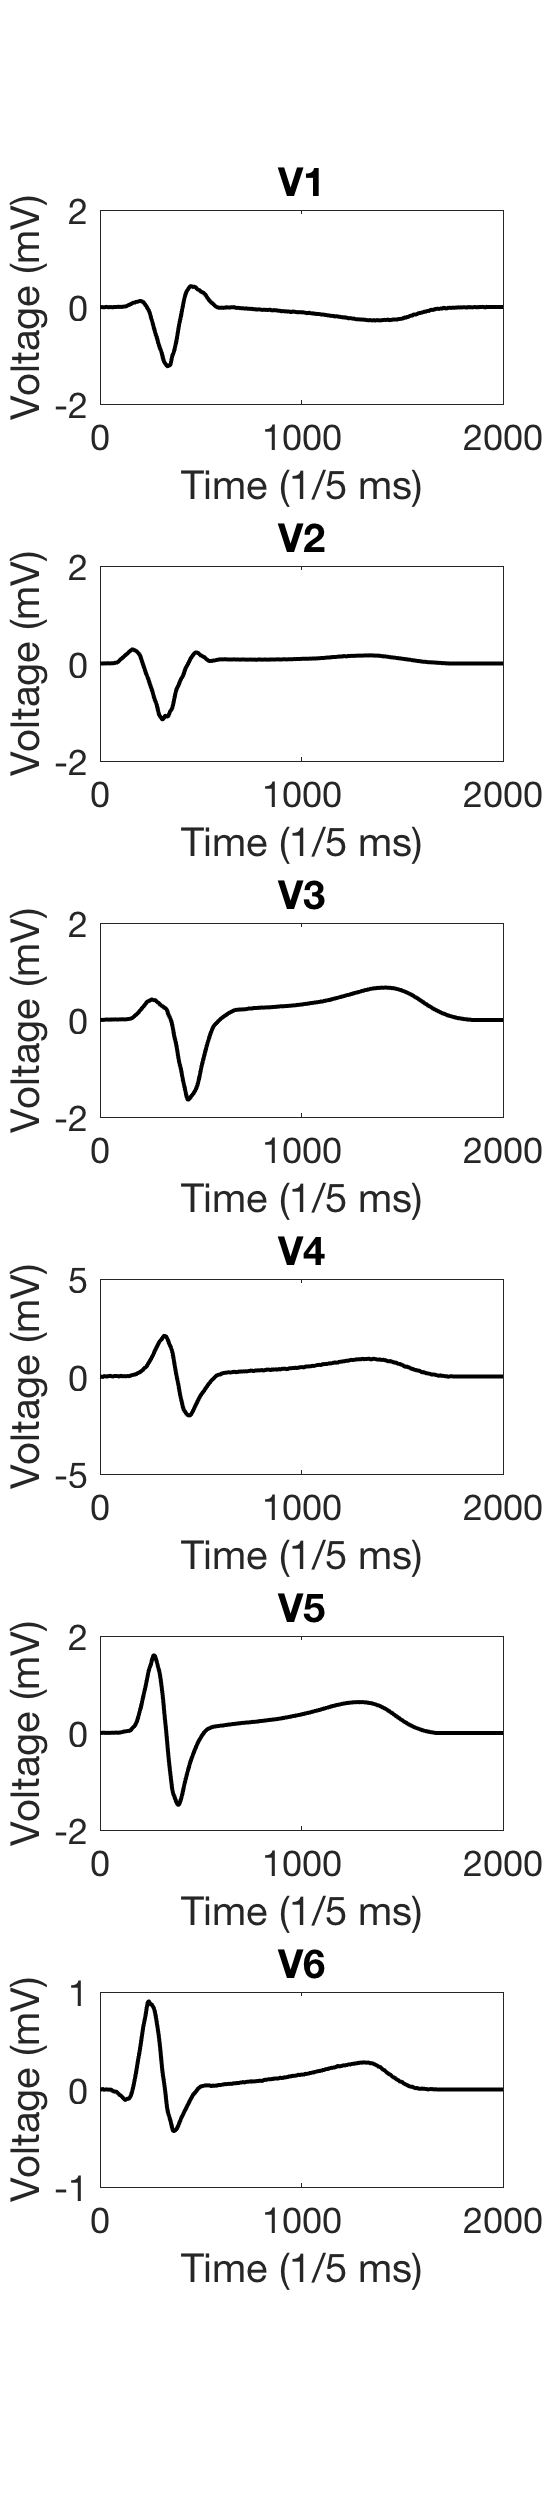
\includegraphics[height = .95\textheight]{Figures/Precordial_timeallign_sigaveraged.png}
	\caption{Signal averaged, filtered, baseline corrected, time aligned precordial leads.}
	\label{fig:PrecordSig}
\end{figure}

\begin{figure}[H]
	
	\centering
	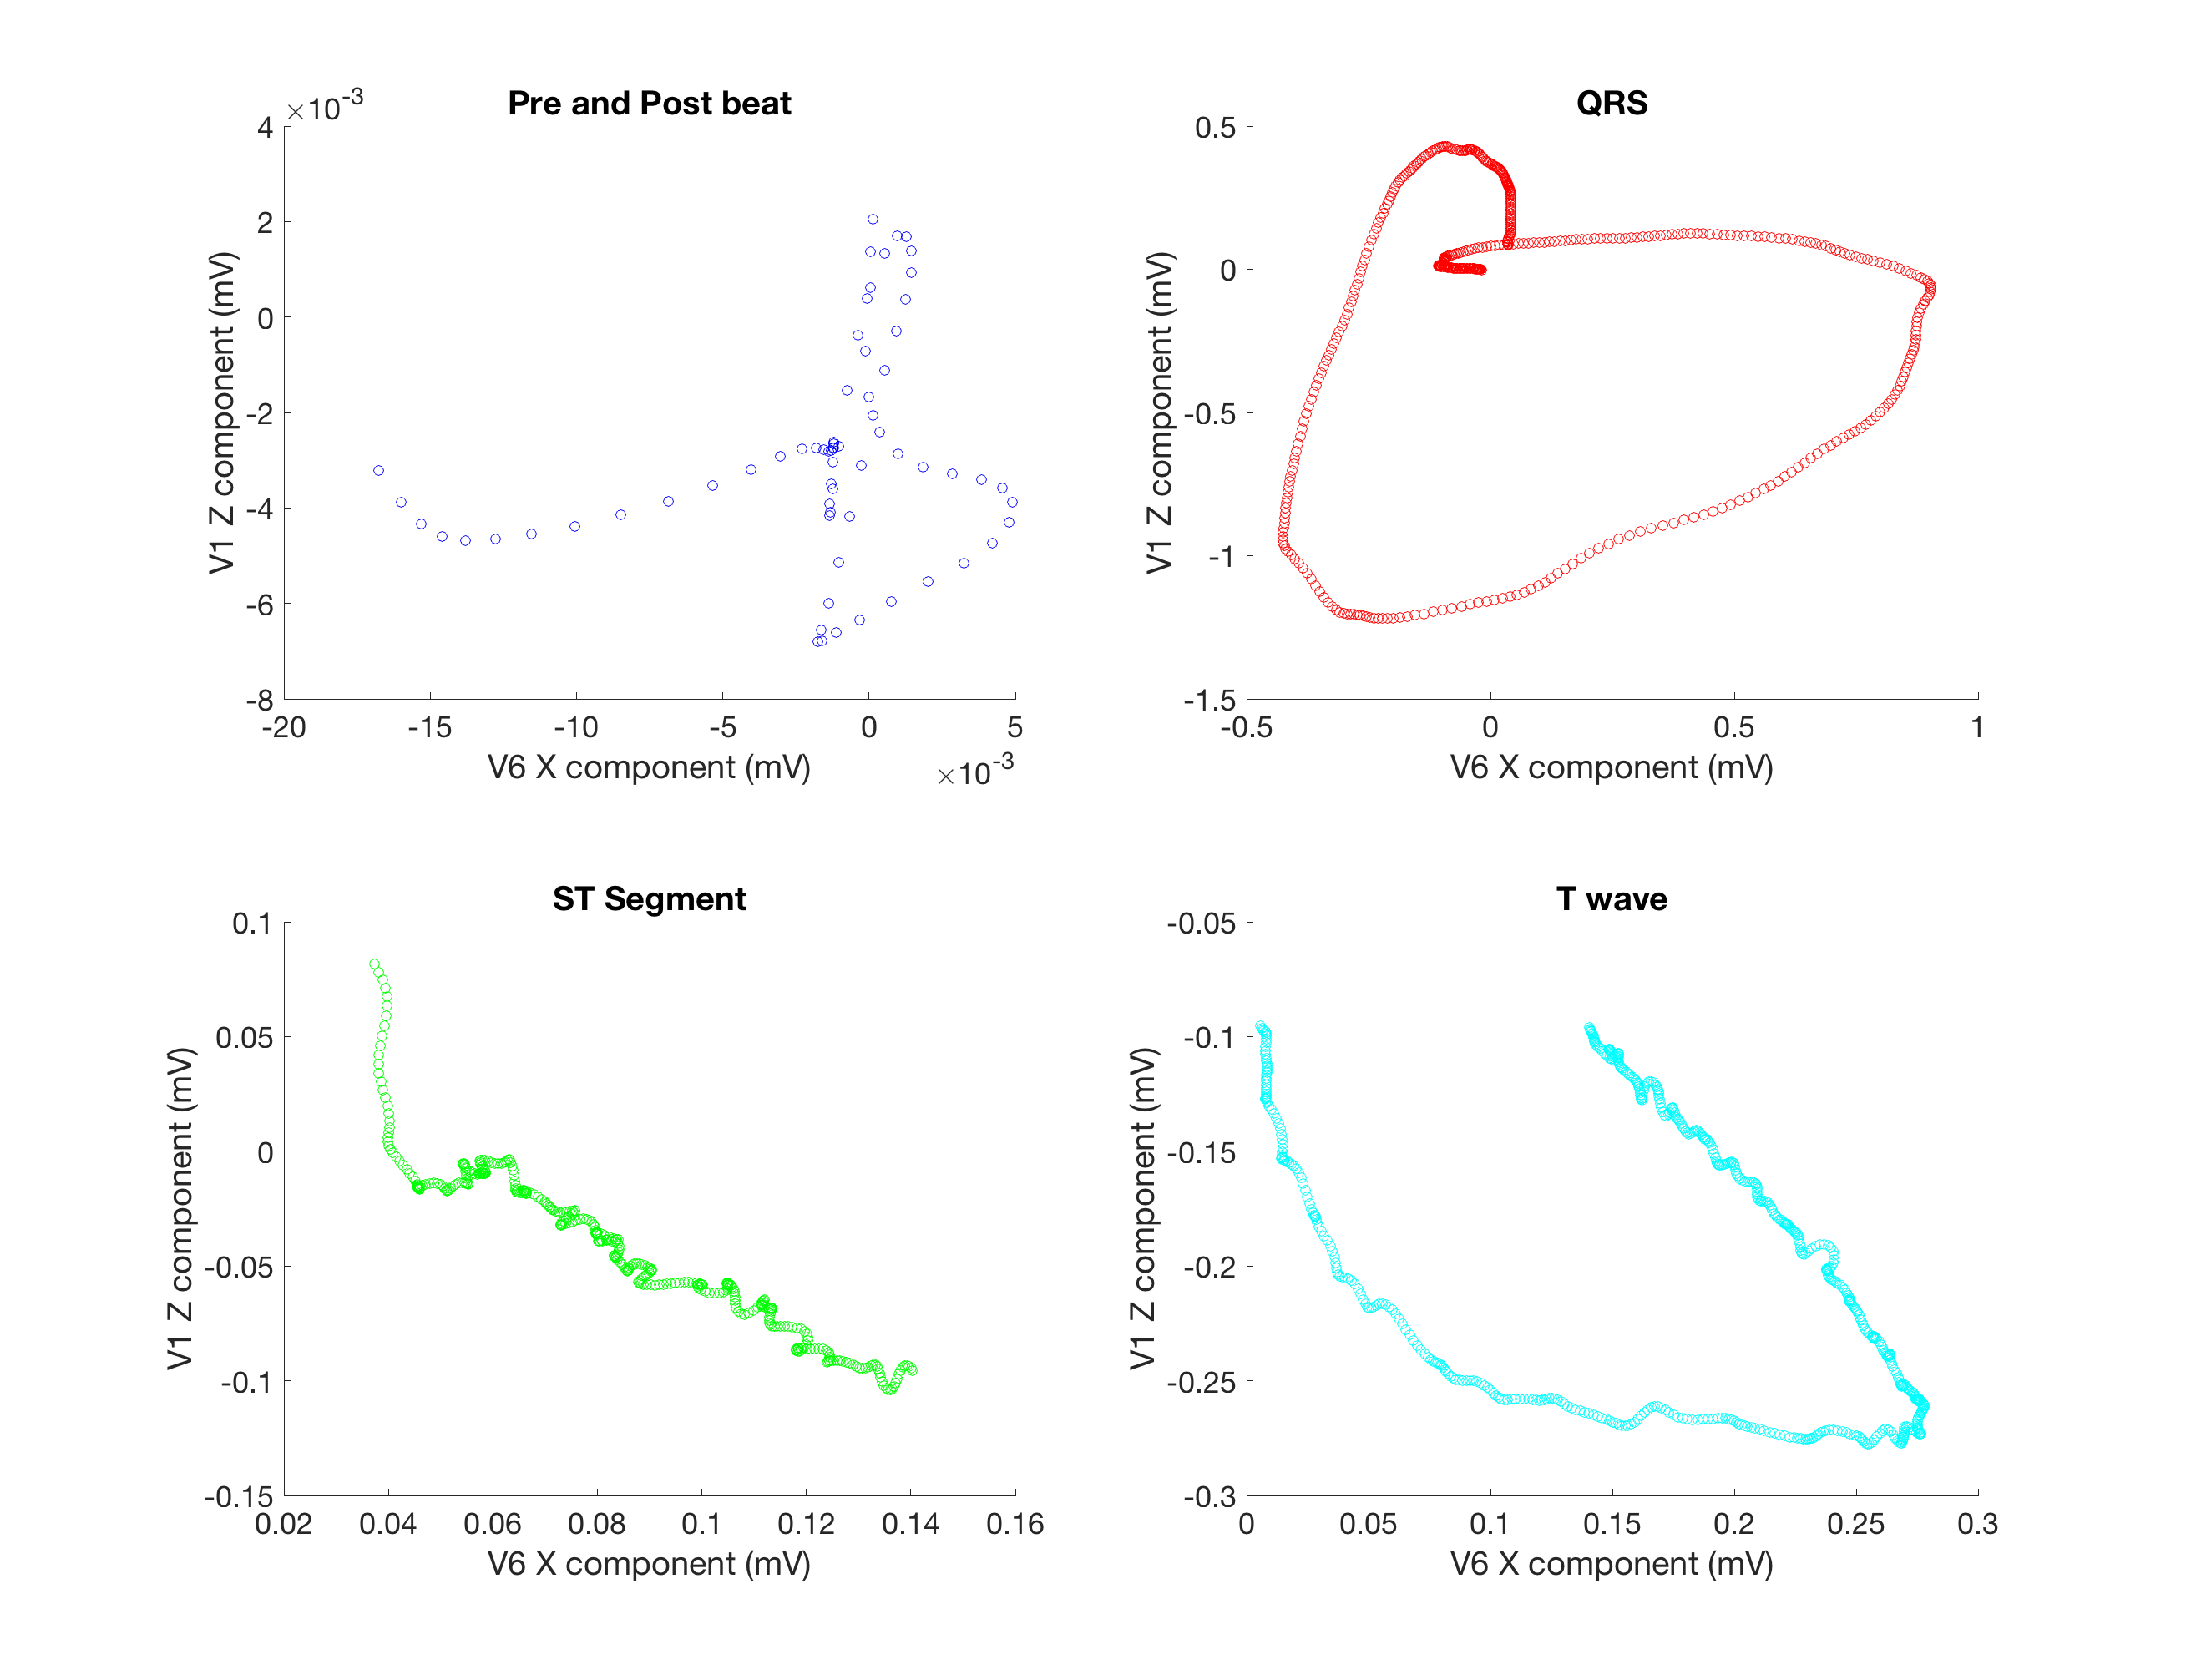
\includegraphics[width = .75\textwidth]{Figures/Precordial_V1V6.png}
	\caption{Precordial VCG using V6 and V1. QRS in Red, ST segment in green, T wave in cyan, isoelectric in blue.}
	\label{fig:PrecordVect}
\end{figure}

\begin{figure}[H]
	
	\centering
	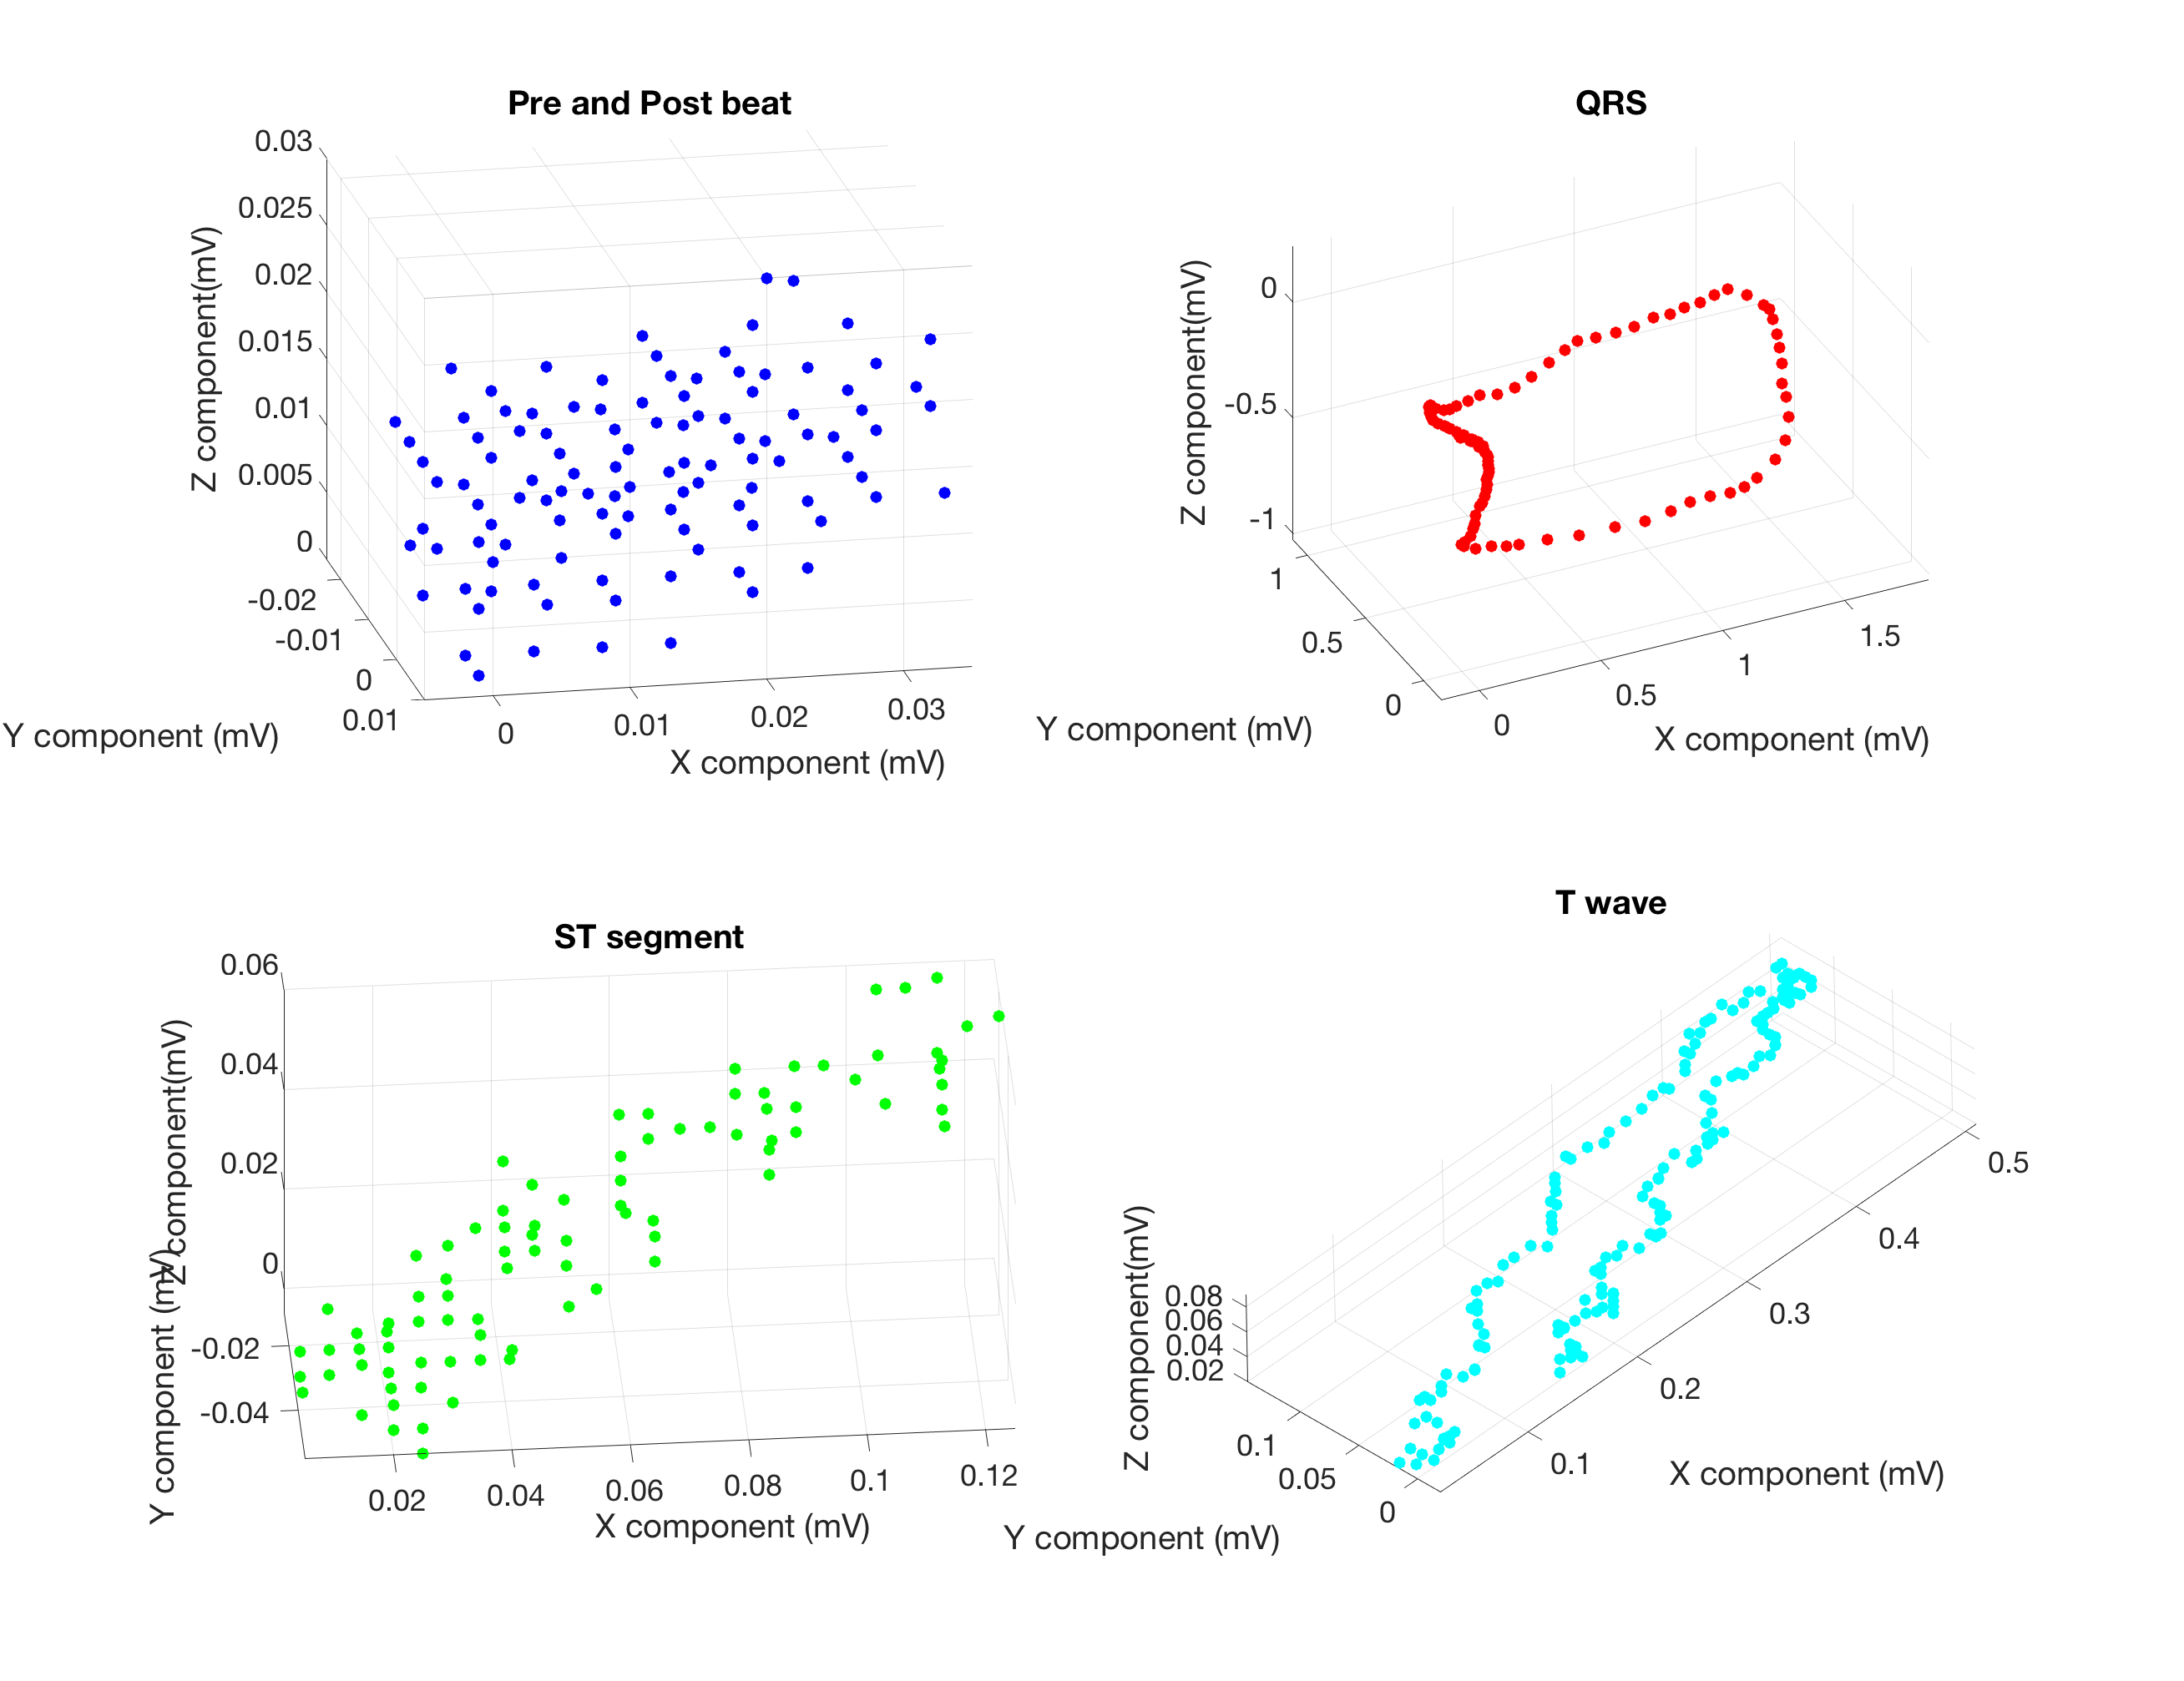
\includegraphics[width = .75\textwidth]{Figures/BSP_run1_3d.png}
	\caption{Body Surface potential VCG in 3D for run 1, lying down. QRS in Red, ST segment in green, T wave in cyan, isoelectric in blue.}
	\label{fig:BSP1}
\end{figure}

\begin{figure}[H]
	
	\centering
	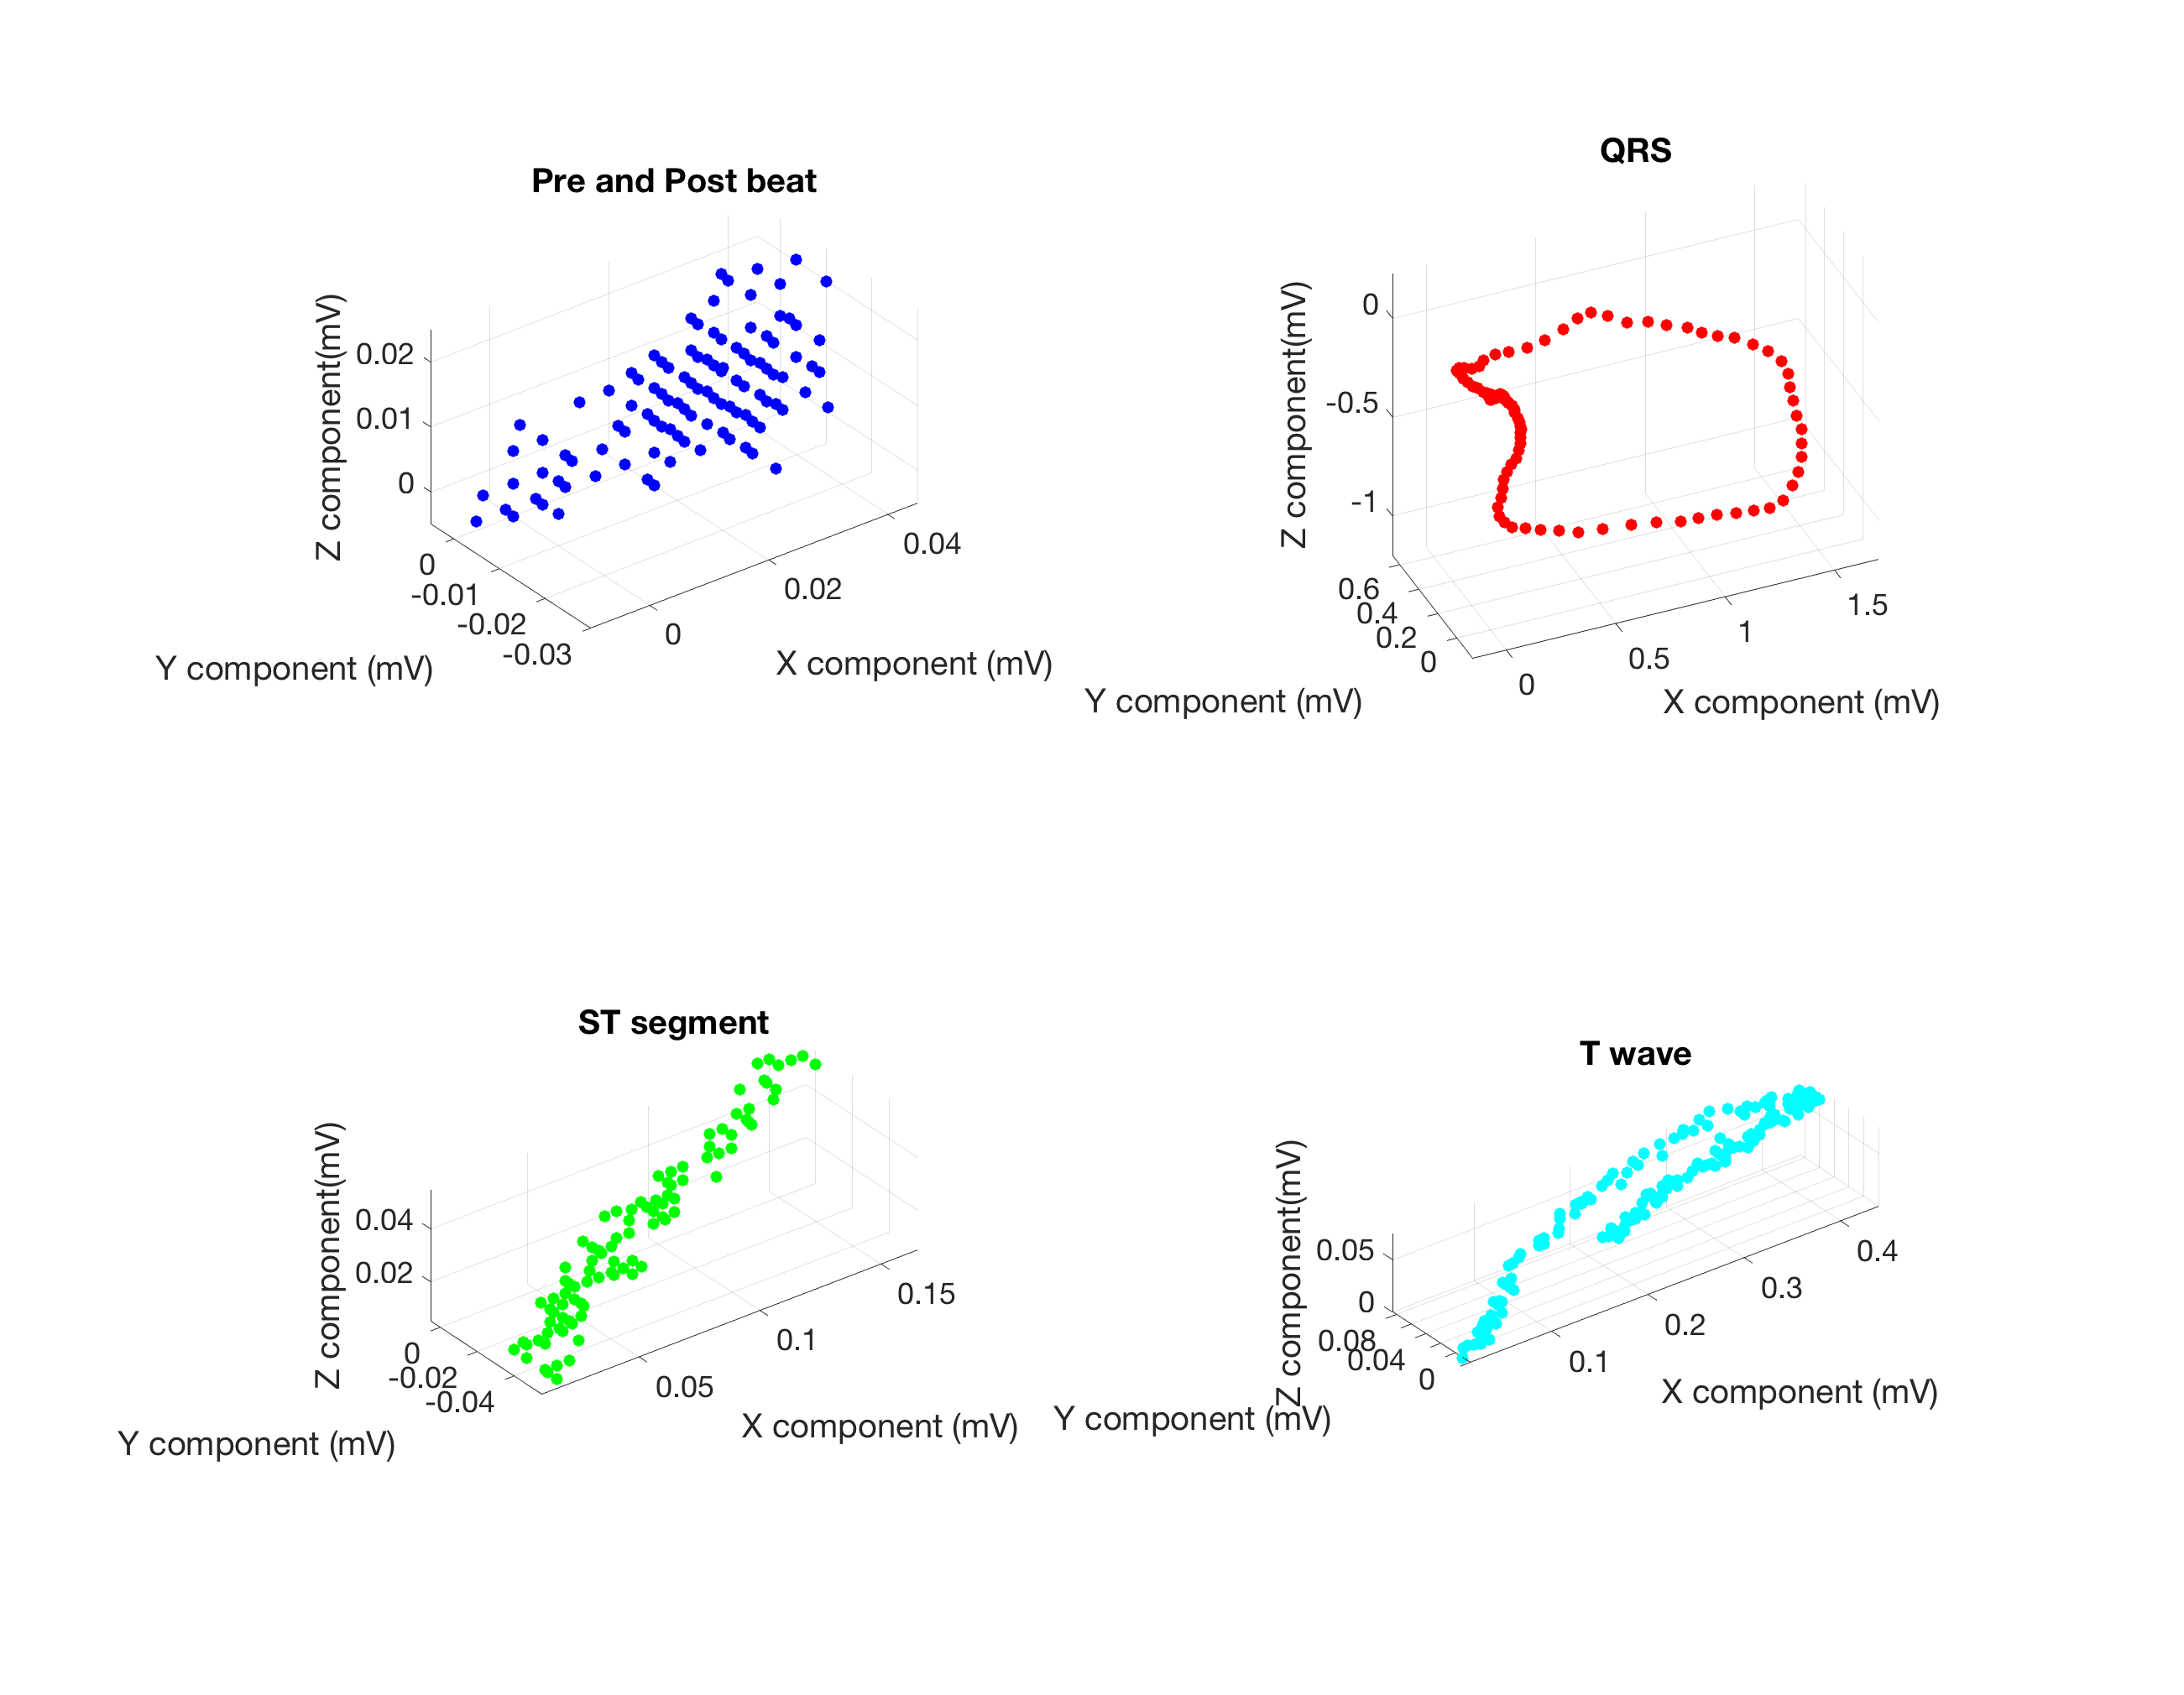
\includegraphics[width = .75\textwidth]{Figures/BSP_run2_3d.png}
	\caption{Body Surface potential VCG in 3D for run 2, sitting up. QRS in Red, ST segment in green, T wave in cyan, isoelectric in blue.}
	\label{fig:BSP2}
\end{figure}

\begin{figure}[H]
	
	\centering
	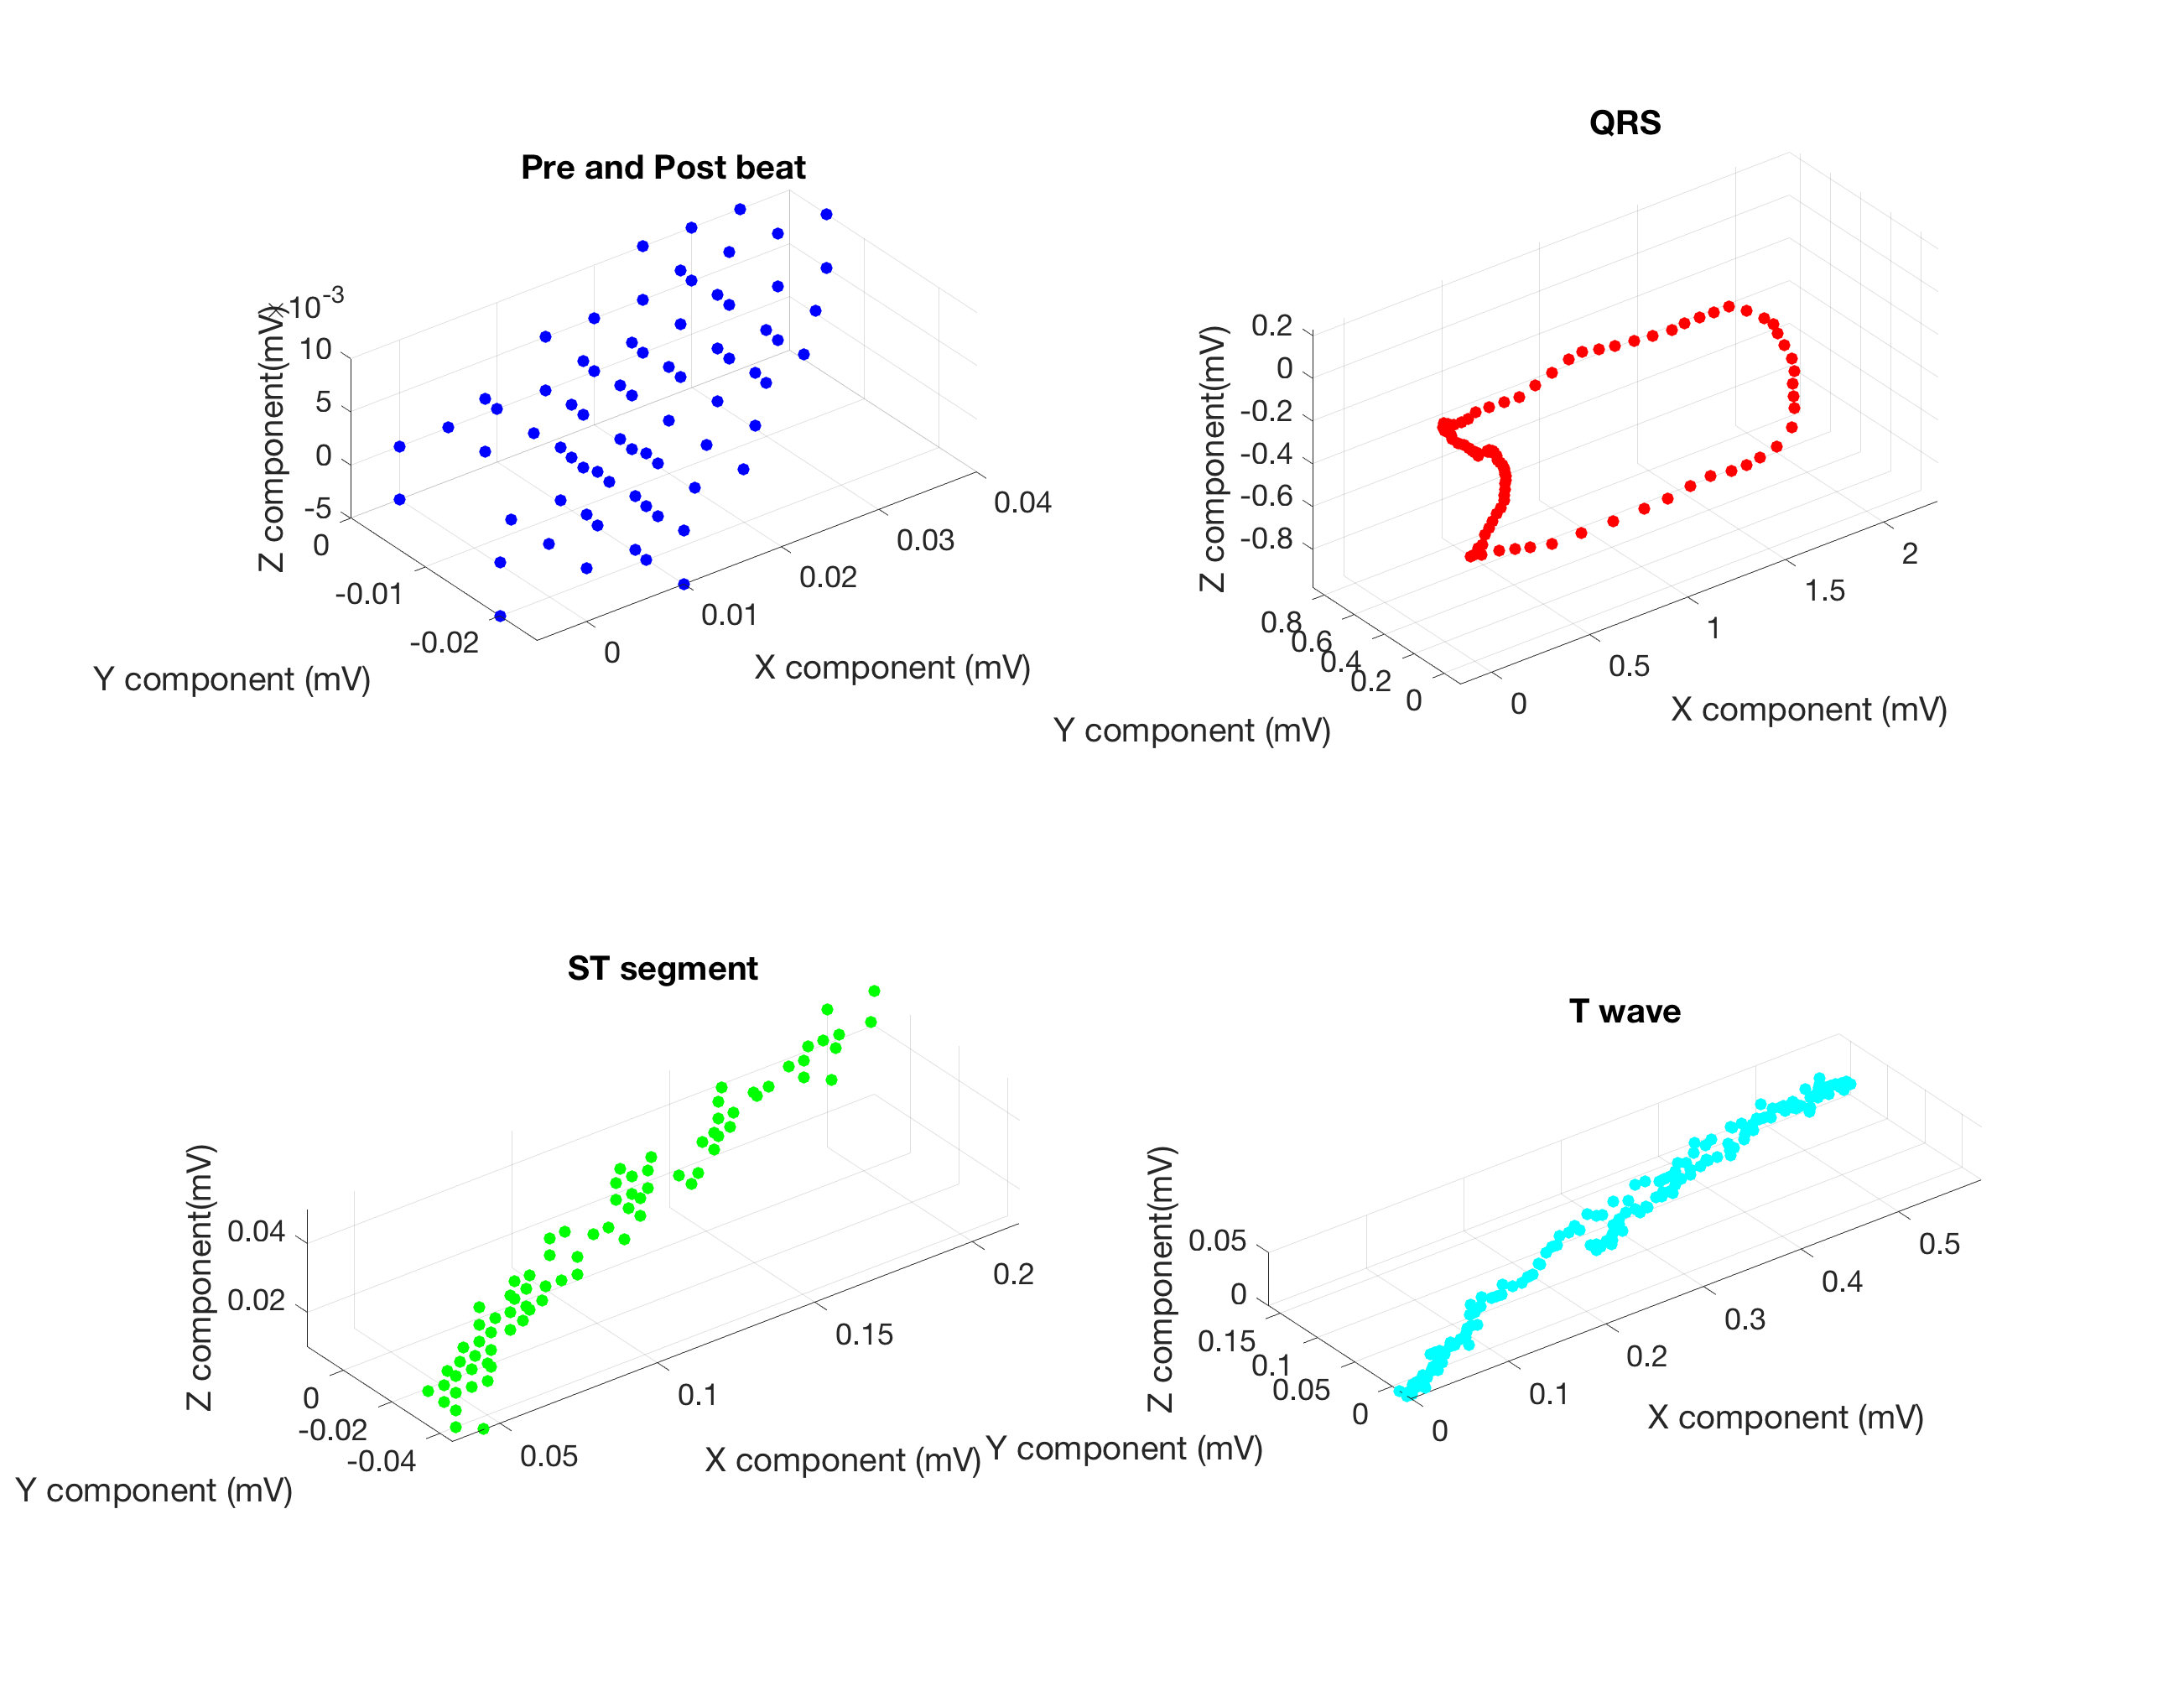
\includegraphics[width = .75\textwidth]{Figures/BSP_run3_3d.png}
	\caption{Body Surface potential VCG in 3D for run 3, lying on the left. QRS in Red, ST segment in green, T wave in cyan, isoelectric in blue. }
	\label{fig:BSP3}
\end{figure}

\begin{figure}[H]
	
	\centering
	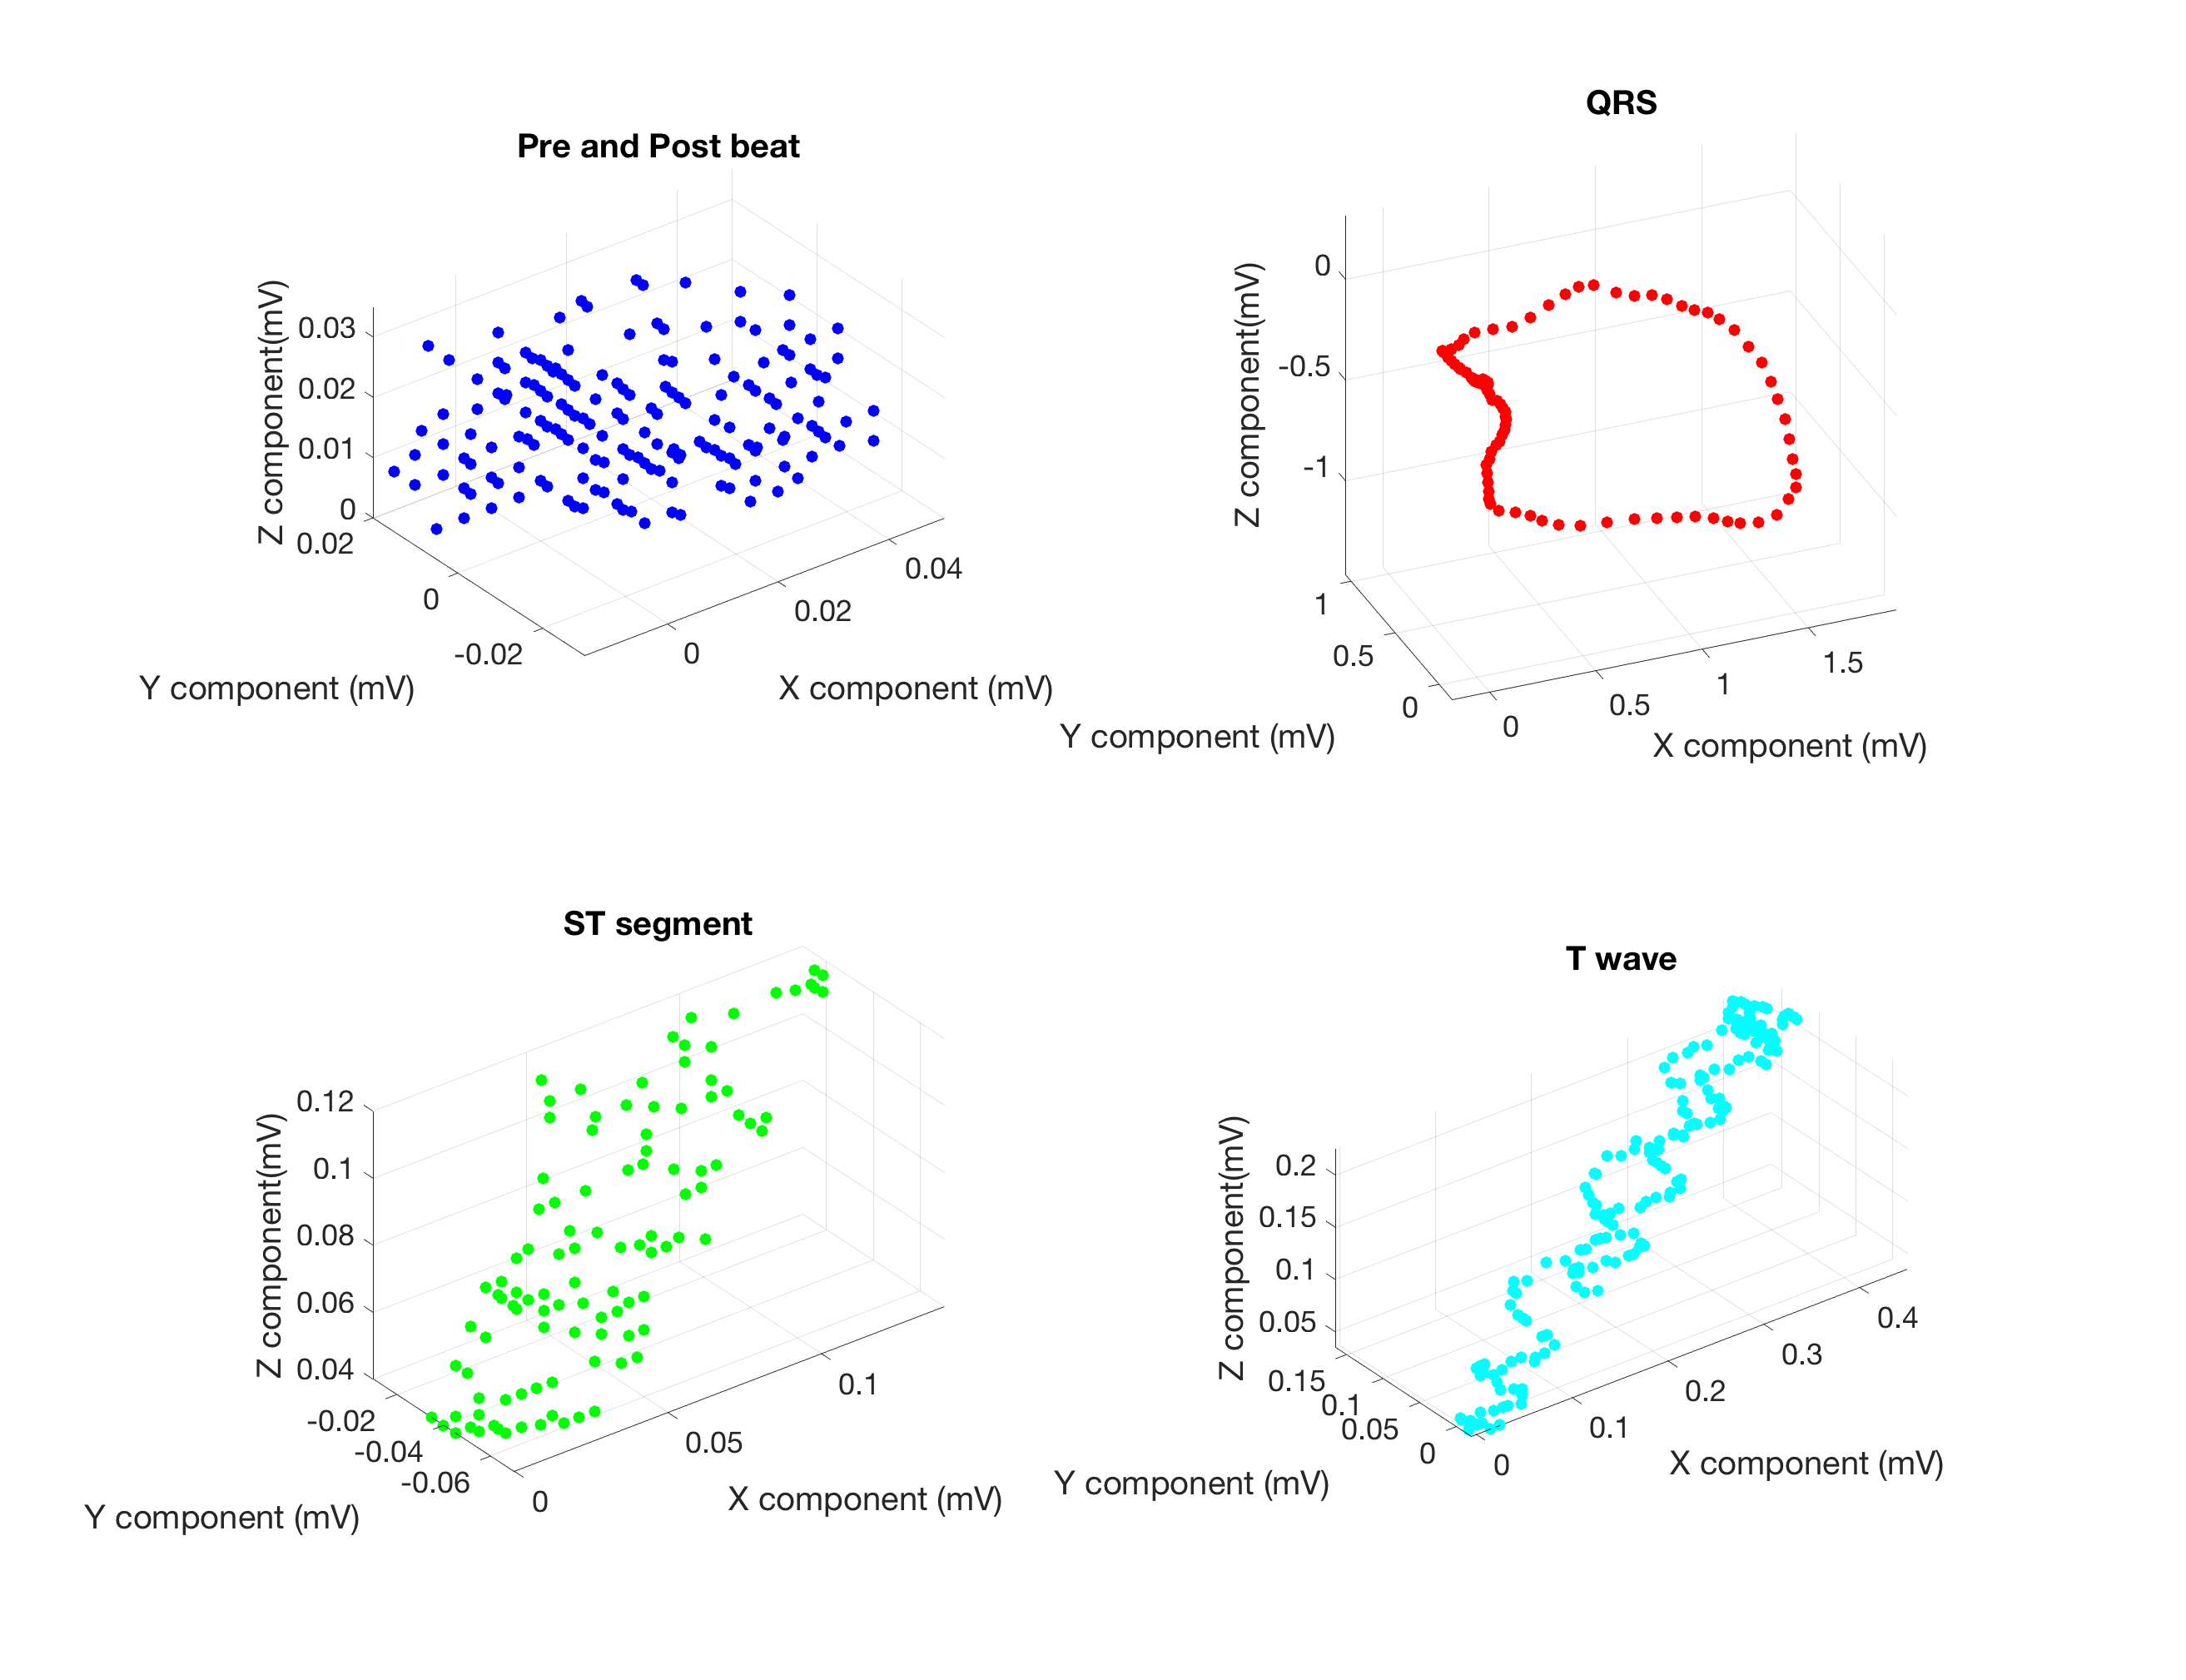
\includegraphics[width = .75\textwidth]{Figures/BSP_run4_3d.png}
	\caption{Body Surface potential VCG in 3D for run 4, lying on the right. QRS in Red, ST segment in green, T wave in cyan, isoelectric in blue. }
	\label{fig:BSP4}
\end{figure}



\section{Discussion}
\par{}
In this lab we sought to investigate the use of various lead sets for assessing ECGs and VCGs. The lead sets we considered were the Limb leads, the Frank orthogonal lead set, and the Precordial lead set with Wilson central terminal as reference. From each of these sets and via our signal processing pipeline we were able to attain high quality ECG signals. 

\par{}
What is interesting to note is that, when comparing the different lead sets, while all were able to produce what appear to be reasonable vector trajectories (large changes during the QRS and T wave, minimal changes in the isoelectric periods and the ST segment) the comparison between lead sets shows vastly different VCGs. Even when comparing similar planar projections such as a comparison between Figure~\ref{fig:Limb5}, and  Figure~\ref{fig:Frank_xy}, both of which show frontal plane projections of the heart vector the actual trajectories and predominant angles with respect to the X or Y axes vary. In both cases the angle of the QRS trajectory is similar but the shape is widely different. The shapes of the ST and T wave trajectories however are strikingly similar. Thus the differences seen in the QRS trajectories likely result from the lead placement differences between these two sets.
\par{}
When making another such lead set comparison, this time between the precordial V6-V1 VCG (Figure~\ref{fig:PrecordVect}) and the Frank coronal plane (Figure~\ref{fig:Frank_xz}) again there are major differences in the trajectories. In both cases the general shapes are similar for the QRS and T wave (inverted for the T wave but this may be due to an axis inversion) but the specific path is not the same.

\par{}
In the body surface mapping data we see that the main trajectory differences arise in the QRS in the different positions. Between all cases the ST segment and the isoelectric periods did not change much, and given the scale of these trajectories they remained mostly near zero. For the T wave and QRS however changes can be seen in particular betwen lying flat (Figure~\ref{fig:BSP1}) and lying on either side (Figure~\ref{fig:BSp3} Figure~\ref{fig:BSp4}). In these cases the QRS trajectory changes in the 3D extent indicating a shift in the heart's position during these recordings.

\par{}
Overall in these results we see that the lead sets allow us to get some idea of the electric activity of the heart, but based on the differences between the different lead set projections, it seems that there is some inconsistency. This may be explained by looking at one of the base assumptions of these VCGs, that the heart can be represented as a simple current dipole source. If this were the case we would not expect to see such complex changes in the VCGs across lead sets that reference the same plane of projection. In this way we can generally assume that the simple dipole source model may be incomplete. That being said, such a model can still be useful as it does seem to hold generally or at some level. We are able to deconstruct the limb leads and get a major dipole vector for the heart. It may just be the case that this vector is an oversimplification of the actual heart activity.
%%%%%%%%%%%%%%%%%% Correct Bibliography Style

\bibliography{C:/Users/Jake/Documents/library}
\bibliographystyle{IEEEtran}


\end{document}








